\documentclass[9pt,pdf,hyperref={unicode}]{beamer}

\mode<presentation>
{
\usetheme{boxes}
\beamertemplatenavigationsymbolsempty
\setbeamertemplate{footline}[page number]
\setbeamersize{text margin left=1em, text margin right=1em}
\setlength{\emergencystretch}{2em}
}

\input{glyphtounicode}\pdfgentounicode=1
\usepackage{cmap}
\usepackage[T2A]{fontenc}
\usepackage[utf8]{inputenc}
\usepackage[english, russian]{babel}
\usepackage{bm}
\usepackage{multirow}
\usepackage{ragged2e}
\usepackage{indentfirst}
\usepackage{multicol}
\usepackage{subfig}
\usepackage{amsmath,amssymb}
\usepackage{mathrsfs}
\usepackage{enumerate}
\usepackage{mathtools}
\usepackage{comment}
\usepackage{color}
\definecolor{python-green}{RGB}{55,126,33}

\usepackage{tikz}
\usetikzlibrary{positioning,arrows}
\usepackage{pgfplots}
\pgfplotsset{compat=1.16,trig format=rad}

\usepackage{caption}
\captionsetup{skip=0pt,belowskip=0pt}

\newtheorem{rustheorem}{Теорема}
\newtheorem{rusdefinition}{Определение}
\newtheorem{rusassumption}{Предположение}
\newtheorem{rusremark}{Замечание}
\newtheorem{ruscorollary}{Следствие}
\newtheorem{rusproposition}{Предложение}
\newtheorem{ruslemma}{Лемма}
\newtheorem{rushypothesis}{Гипотеза}

% colors
\definecolor{darkgreen}{rgb}{0.0, 0.2, 0.13}
\definecolor{darkcyan}{rgb}{0.0, 0.55, 0.55}
\newcommand{\key}[1]{\par\vspace{0.5ex}\noindent\textbf{\color{darkgreen}#1}}

\AtBeginEnvironment{figure}{\setcounter{subfigure}{0}}%

%----------------------------------------------------------------------------------------------------------

\title[Ландшафтная мера сложности моделей и данных]{Ландшафтная мера сложности моделей и данных \\ в параметрических моделях машинного обучения}
\author{А.В.~Грабовой}

\institute[]{Диссертация на соискание ученой степени\\
доктора физико-математических наук\\~\\1.2.1~--- Искусственный интеллект и машинное обучение\\~\\Научный консультант: профессор РАН К.\,В.~Воронцов}
\date[2026]{\small 19\;ноября\;2026\,г.}

%----------------------------------------------------------------------------------------------------------
\begin{document}

\begin{frame}
\titlepage
\end{frame}

%----------------------------------------------------------------------------------------------------------
\section{Цель, задачи, объект и предмет исследования}
%----------------------------------------------------------------------------------------------------------
\begin{frame}{Цель и задачи исследования}
\justifying
\footnotesize
\textbf{Цель:} построение теоретического аппарата оценки согласованности сложности параметрических моделей машинного обучения с характеристиками обучающей выборки и методов снижения сложности таких моделей на основе анализа ландшафта функции потерь.

\vspace{0.3cm}
\textbf{Задачи:}
\begin{itemize}
    \justifying
    \item[--] введение определений мер сложности моделей и выборок на основе аксиоматического введения функционалов сложности и формулировка критерия согласованности модели и выборки.
    \item[--] построение ландшафтной меры сложности модели по матрицам Гессе и установление ее связи с приращением эмпирического риска при изменении выборки.
    \item[--] получение теоретических оценок ландшафтной меры для полносвязных, сверточных и трансформерных архитектур.
    \item[--] построение методов оценки достаточного объема выборки и анализ их связи со сложностью модели через условную сложность выборки и стабилизацию эмпирического риска.
    \item[--] построение методов снижения сложности моделей, опирающихся на локальную геометрию функции потерь.
    \item[--] демонстрация применимости построенного аппарата в прикладных задачах.
\end{itemize}
\end{frame}
%----------------------------------------------------------------------------------------------------------
\begin{frame}{Объект, предмет и методы исследования}
\justifying
\small
\textbf{Объект исследования.} Процесс обучения параметрических моделей машинного обучения по конечным выборкам.

\vspace{0.3cm}
\textbf{Предмет исследования.} Согласованность сложности параметрических моделей машинного обучения с характеристиками обучающей выборки, формализуемая мерами на модели и на выборке.

\vspace{0.3cm}
\textbf{Методы исследования.} Методы теории множеств и функционального анализа, линейной алгебры, матричного анализа, включая матричное дифференцирование и спектральный анализ матриц, методы теории вероятностей, математической статистики, включая байесовский анализ, анализ сходимости случайных процессов, методы теории оптимизации, анализа функций многих переменных, методы статистической теории обучения.
\end{frame}
%----------------------------------------------------------------------------------------------------------
\section{Научная новизна и значимость работы}
%----------------------------------------------------------------------------------------------------------
\begin{frame}{Научная новизна}
\justifying
\footnotesize
\begin{itemize}
    \justifying
    \item Введены формальные определения меры сложности выборки $\mu_D(D)$ и меры сложности модели $\mu_f(f)$ на основе аксиоматического введения функционалов сложности, сформулирован критерий согласованности модели и выборки $\mu_f(f) \le \mu_D(D)$.
    \item Введена ландшафтная мера сложности модели $\mu_f(f|D) = \mathbb{E}_{i}\big\|\mathbf{H}_{i}(\boldsymbol{\theta}^*)-\mathbb{E}_{j}\mathbf{H}_{j}(\boldsymbol{\theta}^*)\big\|_2$, где ожидания берутся по равномерному выбору объектов $i,j$ из выборки~$D$, а $\|\cdot\|_2$~--- спектральная норма матрицы. Мера задает количественную связь между изменением выборки и локальной геометрией оптимизационного ландшафта.
    \item Для полносвязных и сверточных архитектур получены оценки ландшафтной меры через спектральные нормы матриц Гессе, растущие экспоненциально с глубиной и полиномиально с шириной и числом каналов. Для слоя самовнимания получена оценка по компонентам, полиномиальная по норме входов и нормам весов.
    \item Установлена двусторонняя оценка достаточного размера выборки через ландшафтную меру сложности модели и требуемую точность, а условная сложность выборки выражена через достаточный размер выборки.
    \item Предложены прореживание по ковариации градиентов, многодоменная дистилляция и антидистилляция как методы снижения сложности, опирающиеся на локальную геометрию функции потерь. Байесовская дистилляция рассматривается как развитие кандидатской постановки и не выносится отдельным положением на защиту докторской работы.
    \item Для низкоранговой адаптации параметров доказана состоятельность оценки при стандартных условиях. Для многозадачного обучения получено сравнение верхних оценок эмпирической радемахеровской сложности на задачу при справедливом масштабировании нормы энкодера.
\end{itemize}
\end{frame}
%----------------------------------------------------------------------------------------------------------
\begin{frame}{Теоретическая и практическая значимость}
\justifying
\small
\textbf{Теоретическая значимость.} Результаты вписывают локальный анализ матриц Гессе в теорию сложности обучаемости как вычислимый мост между архитектурными параметрами модели и вопросом согласования модели с выборкой, дополняя классические подходы на основе VC-размерности, PAC-обучаемости и радемахеровской сложности в части анализа стабилизации обучения для перепараметризованных моделей.
Полученные оценки ландшафтной меры дают основание для сравнительного анализа архитектур и для сопоставления методов оценки достаточного объема выборки со сложностью модели.
Основной вклад работы состоит в построении ландшафтной меры сложности параметрической модели и в установлении на ее основе вычислимой связи между архитектурой модели, стабилизацией обучения и характеристиками выборки.

\vspace{0.3cm}
\textbf{Практическая значимость.} Разработанный теоретический аппарат применен к решению прикладных задач машинного обучения: многозадачного обучения, декодирования фМРТ-изображений и детекции машинно-генерированного контента.
Полученные методы оценки и снижения сложности моделей и данных экспериментально проверены на реальных задачах компьютерного зрения, обработки естественного языка и классификации.
\end{frame}
%----------------------------------------------------------------------------------------------------------
\section{Постановка и ограничения классических подходов}
%----------------------------------------------------------------------------------------------------------
\begin{frame}{Актуальность оценки сложности}
\justifying
\small
\textbf{Рост сложности моделей.} Сложность моделей глубокого обучения возрастает на порядки с ростом числа обучаемых параметров. Это делает вопрос о соответствии сложности модели сложности данных практически значимым: для таких моделей затруднительно априорно оценить необходимый объем данных и предсказать поведение при обучении.

\textbf{Ограниченность классических мер сложности.} Классические меры сложности --- VC-размерность, радемахеровская сложность и PAC-обучаемость --- характеризуют класс гипотез и ориентированы на анализ худшего случая. Их оценки консервативны для перепараметризованных моделей и не учитывают специфику архитектур, что ограничивает их применимость к моделям глубокого обучения.

\textbf{Независимость от найденного решения.} VC-размерность и радемахеровская сложность класса не зависят от найденного решения $f\in\mathcal{F}$ и не отражают влияния регуляризации, ранней остановки и особенностей процесса оптимизации на обобщающую способность модели.

\textbf{О границе применимости.} Результаты формулируются в терминах стабилизации эмпирического риска, утверждения о связи с обобщающей способностью в работе не доказываются.

\textbf{Сведение сложности данных к объему выборки.} Существующие подходы к оценке сложности данных сводят ее к размеру обучающей выборки, не учитывая сложность отдельных объектов.

\textbf{Отсутствие единого критерия.} Отсутствует единый теоретический аппарат, связывающий сложность модели и сложность данных формальным критерием согласованности.

\vspace{0.15cm}
\textbf{Ключевая проблема:} построить формальный критерий согласованности сложности модели~$\mu_f(f)$ и сложности данных~$\mu_D(D)$.
\end{frame}
%----------------------------------------------------------------------------------------------------------
%----------------------------------------------------------------------------------------------------------
\begin{frame}{Недостатки меры сложности классов}
\justifying
\small
\textbf{Проблема.} Классические меры относятся к классу гипотез, а не к конкретному решению. Для перепараметризованных сетей оценки завышают сложность обобщения.

\textbf{VC-размерность.} Наибольшее число точек, которые класс может разбить всеми способами. Функция роста:
\[
    m_{\mathcal{H}}(n)=\sum_{i=0}^{VC(\mathcal{H})}\binom{n}{i}.
\]
\textbf{Радемахеровская сложность.} Ожидаемая корреляция класса со случайными знаками $\boldsymbol{\sigma}=\pm1$:
\[
    \widehat{\mathfrak R}_S(\mathcal{H})=\mathbb{E}_{\boldsymbol{\sigma}}\sup_{h\in\mathcal{H}}\frac{1}{n}\sum_{i=1}^{n}\sigma_i\,h(\mathbf{x}_i).
\]
\textbf{PAC-граница.} С вероятностью $1-\delta$:
\[
    R(f)\le \widehat R_S(f)+2\,\widehat{\mathfrak R}_S(\mathcal{H})+3\sqrt{\frac{\log(2/\delta)}{2n}}.
\]
\begin{block}{Свойства}
\begin{itemize}
    \item $VC(\mathcal{H})$ и $\widehat{\mathfrak R}_S(\mathcal{H})$ растут с размерностью класса.
    \item не зависят от конкретного решения $f\in\mathcal{F}$.
\end{itemize}
\end{block}
\key{Классические меры относятся к классу гипотез, а не к конкретному решению.}
\end{frame}
%----------------------------------------------------------------------------------------------------------
\begin{frame}{Недостатки аппроксимационной теории}
\justifying
\small
\textbf{Проблема.} Существование аппроксиматора не гарантирует, что обучение по конечной выборке его найдет. Аппроксимация отвечает на вопрос о реализуемости, а не о сложности обучения.
Универсальная аппроксимация (Цибенко, 1989): сеть с одним скрытым слоем аппроксимирует любую непрерывную функцию. Рост выразительности с глубиной (Хестад, 1987, Бенджио, 2007).
\begin{rustheorem}
    Пусть $\sigma$ --- непрерывная ограниченная неконстантная функция, $f\in C[0,1]^d$, $\varepsilon>0$. Тогда существует $N$, матрицы $\mathbf{W}_1,\mathbf{W}_2$ и вектор $\mathbf{b}$ такие, что
    \[
        \bigl\|\mathbf{W}_2\sigma(\mathbf{W}_1\mathbf{x}+\mathbf{b})-f(\mathbf{x})\bigr\|_\infty<\varepsilon\quad\forall\mathbf{x}\in[0,1]^d.
    \]
\end{rustheorem}
Разложение полной ошибки обученной модели~$f_D$:
\[
    R(f_D)\le R(f^*)+\underbrace{\inf_{f\in\mathcal{F}}R(f)-R(f^*)}_{\text{ошибка аппроксимации}}+\underbrace{\bigl(R(f_D)-\inf_{f\in\mathcal{F}}R(f)\bigr)^{+}}_{\text{ошибка оценивания}},
\]
где $f^*$ --- функция, реализующая минимум истинного риска.

\key{Аппроксимационная теория не задает сложность обучения по конечной выборке.}
\end{frame}
%----------------------------------------------------------------------------------------------------------
\begin{frame}[t]{Недостатки законов масштабирования}
\small
\textbf{Проблема.} Законы масштабирования не объясняют механизм обобщения: $N$ агрегирует неоднородные степени свободы.
\[
    L(N,D,C)\approx L_{\infty}+aN^{-\alpha}+bD^{-\beta}+cC^{-\gamma}.
\]
При фиксированном бюджете $C$ из $D=C/N$ условие $\partial L/\partial N=0$ задает оптимум:
\[
    N^{*}\propto C^{\frac{\beta}{\alpha+\beta}},\qquad
    D^{*}=\frac{C}{N^{*}}\propto C^{\frac{\alpha}{\alpha+\beta}}.
\]

\begin{minipage}[c]{0.46\textwidth}\centering
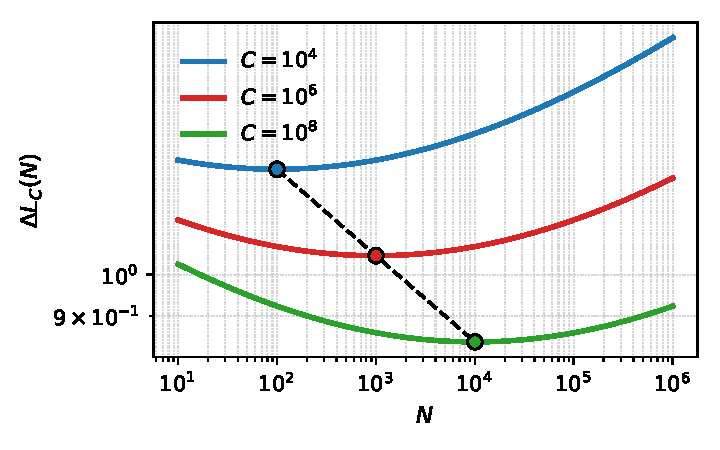
\includegraphics[width=0.98\textwidth]{thesis/figures/chapter-0/scaling_law.pdf}
\end{minipage}\hfill
\begin{minipage}[c]{0.50\textwidth}
Каждая кривая --- фиксированный $C$, минимум в~$N^{*}$. С ростом $C$ минимум смещается вправо и вниз.
\end{minipage}
\key{Законы масштабирования --- эмпирическое макроописание без объяснения механизма.}
\end{frame}
%----------------------------------------------------------------------------------------------------------
\begin{frame}{Параметрические семейства функций}
\justifying
\footnotesize

Рассмотрим параметрическое отображение $f_{\boldsymbol{\theta}}:\mathcal{X}\to\mathcal{Y}$, аппроксимирующее условное распределение целевой переменной $p(\mathbf{y}|\mathbf{x})$. Параметры $\boldsymbol{\theta}$ принадлежат пространству $\mathbb{R}^{P}$, где $P$ описывает число параметров отображения $f_{\boldsymbol{\theta}}$.

\begin{rusdefinition}
    \textbf{Генеральной совокупностью данных}~$\Gamma$ назовем произвольное множество объектов, которые исследуются в рамках той или иной задачи. В общем случае нет никаких ограничений на счетность множества генеральной совокупности.
\end{rusdefinition}

\begin{rusdefinition}
    Генеральную совокупность~$\Gamma$ назовем \textbf{однородной}, если все ее объекты порождаются из одного распределения. В противном случае назовем ее \textbf{гетерогенной}. Если совокупность образуется~$k$ различными распределениями, будем говорить о~$k$-компонентной совокупности.
\end{rusdefinition}

Пусть для выбора оптимального вектора параметров~$\hat{\boldsymbol{\theta}}$ используется подход минимизации эмпирического риска:
\[
    \hat{\boldsymbol{\theta}}=\arg\min_{\boldsymbol{\theta}}\ \mathcal{L}_m(\boldsymbol{\theta}),\qquad
    \mathcal{L}_m(\boldsymbol{\theta})=\frac{1}{m}\sum_{i=1}^{m}\ell\bigl(f_{\boldsymbol{\theta}}(\mathbf{x}_i),\mathbf{y}_i\bigr).
\]

\key{Объект исследования --- параметрические семейства функций, аппроксимирующие данные минимизацией эмпирической функции потерь.}
\end{frame}

%----------------------------------------------------------------------------------------------------------
\section{К ландшафтной мере}
%----------------------------------------------------------------------------------------------------------
\begin{frame}{Изменение ландшафта при вариации выборки}
\justifying
\small
Эмпирический риск на выборках~$k$ и~$k+1$:
\[
    \mathcal{L}_k(\boldsymbol{\theta})=\frac{1}{k}\sum_{i=1}^{k}\ell\bigl(f_{\boldsymbol{\theta}}(\mathbf{x}_i),\mathbf{y}_i\bigr),\qquad
    \mathcal{L}_{k+1}(\boldsymbol{\theta})=\frac{1}{k+1}\sum_{i=1}^{k+1}\ell\bigl(f_{\boldsymbol{\theta}}(\mathbf{x}_i),\mathbf{y}_i\bigr).
\]
\begin{columns}[c]
\begin{column}{0.60\textwidth}
\scriptsize
Изменение при добавлении одного объекта:
\begin{align*}
    \mathcal{L}_{k+1}(\boldsymbol{\theta})-\mathcal{L}_k(\boldsymbol{\theta})
    &=\frac{1}{k+1}\Bigl(\ell\bigl(f_{\boldsymbol{\theta}}(\mathbf{x}_{k+1}),\mathbf{y}_{k+1}\bigr)-\mathcal{L}_k(\boldsymbol{\theta})\Bigr).
\end{align*}
Вклад нового объекта: его ошибка за вычетом среднего по первым~$k$ объектам, деленная на~$k+1$.
\end{column}
\begin{column}{0.40\textwidth}
\begin{center}
\begin{tikzpicture}[scale=0.5,>=stealth]
    \draw[->,thick] (-2.7,0) -- (2.7,0) node[right,black]{$\theta$};
    \draw[->,thick] (0,-0.2) -- (0,1.85) node[above,black]{$\mathcal{L}$};
    \draw[dashed,gray] (0,0) -- (0,1.7);
    \node[below,black] at (0,-0.06) {$\theta^*$};
    \draw[darkcyan,very thick] plot[domain=-1.8:1.8,samples=120] (\x,{0.4*\x*\x+0.18});
    \draw[darkgreen,very thick] plot[domain=-1.8:1.8,samples=120] (\x,{0.5*\x*\x+0.55});
    \draw[<->,red,very thick] (0.7,{0.4*0.7*0.7+0.18}) -- (0.7,{0.5*0.7*0.7+0.55});
    \node[red,align=center] at (0.0,1.28) {$\bigl|\mathcal{L}_{k+1}-\mathcal{L}_k\bigr|$};
    \node[darkcyan,anchor=east] at (-1.9,{0.4*1.8*1.8+0.18}) {$\mathcal{L}_k$};
    \node[darkgreen,anchor=west] at (1.9,{0.5*1.8*1.8+0.55}) {$\mathcal{L}_{k+1}$};
\end{tikzpicture}
\end{center}
\end{column}
\end{columns}
Оценка по неравенству треугольника:
\begin{align*}
    \bigl|\mathcal{L}_{k+1}(\boldsymbol{\theta})-\mathcal{L}_k(\boldsymbol{\theta})\bigr|
    &\le \frac{2M_{\ell}}{k+1}\\
    &\quad+\frac{1}{2(k+1)}\bigl\|\boldsymbol{\theta}-\boldsymbol{\theta}^*\bigr\|_2^2
        \Bigl\|\mathbf{H}_{k+1}(\boldsymbol{\theta}^*)-\frac{1}{k}\sum_{i=1}^{k}\mathbf{H}_{i}(\boldsymbol{\theta}^*)\Bigr\|_2 .
\end{align*}
Слагаемое с нормой матрицы Гессе задает скорость стабилизации ландшафта.

\key{Приращение риска --- вклад нового объекта за вычетом среднего. Скорость сходимости задается нормой разности матриц Гессе.}
\end{frame}
%----------------------------------------------------------------------------------------------------------
\begin{frame}{Стационарность точки минимума}
\justifying
\footnotesize
\begin{rusassumption}
    Пусть $\boldsymbol{\theta}^*$ является стационарной точкой обеих эмпирических функций потерь $\mathcal{L}_{k}(\boldsymbol{\theta})$ и $\mathcal{L}_{k+1}(\boldsymbol{\theta})$, т.е.
    \[
        \nabla \mathcal{L}_{k}(\boldsymbol{\theta}^*) = \nabla \mathcal{L}_{k+1}(\boldsymbol{\theta}^*) = \mathbf{0}.
    \]
\end{rusassumption}

Воспользуемся квадратичным приближением Тейлора в окрестности $\boldsymbol{\theta}^*$:
\[
    \mathcal{L}_k(\boldsymbol{\theta})\approx\mathcal{L}_k(\boldsymbol{\theta}^*)+\frac12(\boldsymbol{\theta}-\boldsymbol{\theta}^*)^\top\mathbf{H}^{(k)}(\boldsymbol{\theta}^*)(\boldsymbol{\theta}-\boldsymbol{\theta}^*),
\]
где $\mathbf{H}^{(k)}(\boldsymbol{\theta}^*)\in\mathbb{R}^{P\times P}$.

Полная матрица Гессе записывается как среднее матриц Гессе отдельных членов:
\[
    \mathbf{H}^{(k)}(\boldsymbol{\theta})=\nabla^2_{\boldsymbol{\theta}}\mathcal{L}_{k}(\boldsymbol{\theta})=\frac{1}{k}\sum_{i=1}^{k}\mathbf{H}_{i}(\boldsymbol{\theta}).
\]
\begin{rusremark}
    Вместо стационарности можно допускать малые градиенты: для некоторого $\varepsilon_g\ge 0$
    \[
        \bigl\|\nabla \mathcal{L}_k(\boldsymbol{\theta}^*)\bigr\|_2 \le \varepsilon_g,\qquad
        \bigl\|\nabla \mathcal{L}_{k+1}(\boldsymbol{\theta}^*)\bigr\|_2 \le \varepsilon_g .
    \]
    Это ослабление существенно не меняет результатов, но для простоты далее используется более сильное ограничение $\varepsilon_g=0$.
\end{rusremark}
\key{Скорость сходимости ландшафта задается разностью матриц Гессе в точке минимума.}
\end{frame}
%----------------------------------------------------------------------------------------------------------
\begin{frame}{Форма дна и рваный рельеф: от ландшафта к мере $\mu_f$}
\justifying
\small
\begin{center}
\begin{tikzpicture}
\begin{axis}[width=0.44\textwidth,height=0.30\textwidth,view={30}{38},colormap={cool}{rgb255(0cm)=(56,79,211); rgb255(1cm)=(226,18,18)},
  title={\footnotesize мало данных, глубокая сеть},
  xlabel=\scriptsize$\theta_1$,ylabel=\scriptsize$\theta_2$,
  xmin=-2,xmax=2,ymin=-2,ymax=2,zmin=-1.6,zmax=1.6,xtick=\empty,ytick=\empty,ztick=\empty,axis lines=none,]
\addplot3[surf,shader=faceted,faceted color=gray!60,domain=-2:2,samples=60]
  {0.55*sin(2.2*x)*sin(1.9*y) + 0.38*sin(3.8*x+1.0*y) + 0.32*sin(1.8*x-3.2*y) + 0.22*sin(5.0*x)*sin(3.4*y) + 0.15*sin(6.6*x+2.6*y)};
\end{axis}
\end{tikzpicture}
\hspace{0.01\textwidth}$\;\xrightarrow{\;\text{больше данных}\;}$\;\hspace{0.01\textwidth}
\begin{tikzpicture}
\begin{axis}[width=0.44\textwidth,height=0.30\textwidth,view={30}{38},colormap={cool}{rgb255(0cm)=(56,79,211); rgb255(1cm)=(226,18,18)},
  title={\footnotesize много данных, широкая сеть},
  xlabel=\scriptsize$\theta_1$,ylabel=\scriptsize$\theta_2$,
  xmin=-2,xmax=2,ymin=-2,ymax=2,zmin=-1.6,zmax=1.6,xtick=\empty,ytick=\empty,ztick=\empty,axis lines=none,]
\addplot3[surf,shader=faceted,faceted color=gray!60,domain=-2:2,samples=40]
  {0.30*(x^2+y^2) + 0.05*(x-y) + 0.10*sin(2.5*x)*sin(2.5*y)};
\end{axis}
\end{tikzpicture}
\end{center}
\vspace{2pt}
{\small\textit{Ландшафт потерь --- как горная местность: чем больше данных, тем ровнее рельеф.}}
\begin{itemize}
    \setlength{\itemsep}{1pt}
    \item Рваный рельеф --- много локальных минимумов и большая норма разности Гессе.
    \item Гладкая долина --- широкая, минимум устойчив к сдвигу от $\theta^*$.
    \item Разброс формы по выборке и есть мера $\mu_f$: чем он меньше, тем ровнее ландшафт.
\end{itemize}
\key{Рваный ландшафт --- большая $\mu_f$, гладкий --- малая.}
\end{frame}
%----------------------------------------------------------------------------------------------------------
\begin{frame}{Ландшафтная мера сложности модели}
\justifying
\small
\begin{rusdefinition}
    Пусть $\mathbf{H}_i(\boldsymbol{\theta}) = \nabla^2_{\boldsymbol{\theta}} \ell(f_{\boldsymbol{\theta}}(\mathbf{x}_i),\mathbf{y}_i)$. Ландшафтная мера сложности задается выражением
    \[
        \mu_f(f\mid D) = \mathbb{E}_{i}\left\| \mathbf{H}_{i}(\boldsymbol{\theta}^*) - \mathbb{E}_{j}\mathbf{H}_{j}(\boldsymbol{\theta}^*) \right\|_2,
    \]
    где $\mathbb{E}_{i}$ означает математическое ожидание по равномерно выбранному индексу из $D$ при фиксированной точке $\boldsymbol{\theta}^*$.
\end{rusdefinition}
\begin{rusremark}
    \begin{itemize}
        \item $\mu_f$ велика, когда пообъектные матрицы Гессе существенно расходятся в операторной норме относительно своего среднего по $D$.
        \item Разность $\mathbf{H}^{(k+1)}-\mathbf{H}^{(k)}$ задает скорость сходимости ландшафта.
        \item Мера фиксируется на найденном решении $\boldsymbol{\theta}^*$ и зависит от параметризации.
        \item Для однозначности рассматривается каноническая параметризация с фиксированной нормировкой весов.
    \end{itemize}   
\end{rusremark}
\begin{figure}[t]\center
    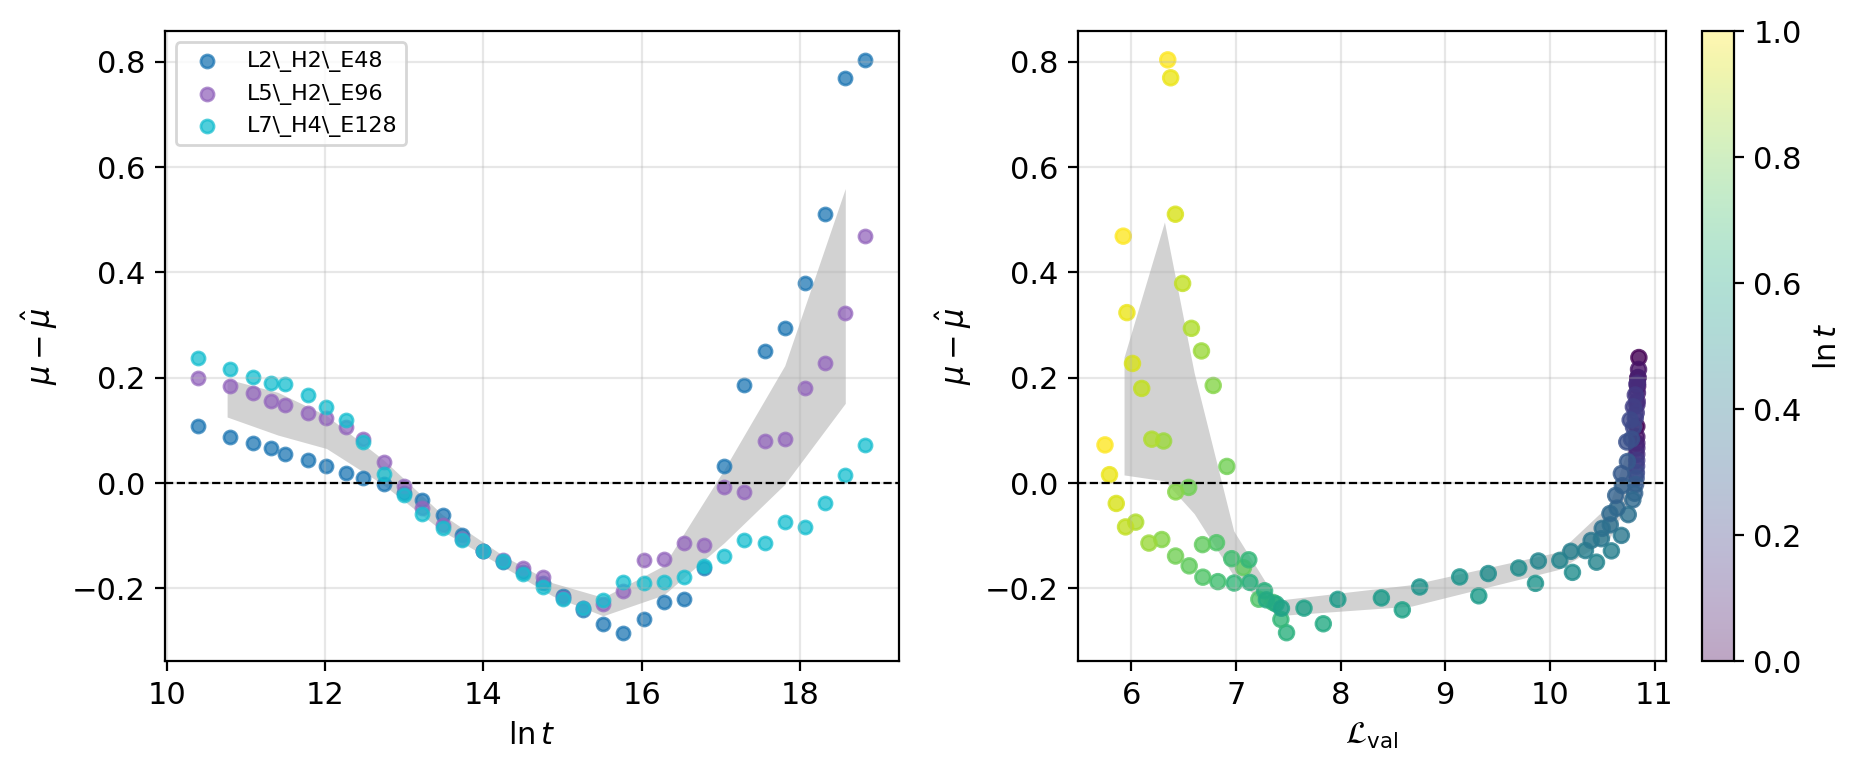
\includegraphics[height=0.17\textwidth]{thesis/figures/chapter-1/empirical-landscape/fig_mu_residual_vs_loss_time.png}
    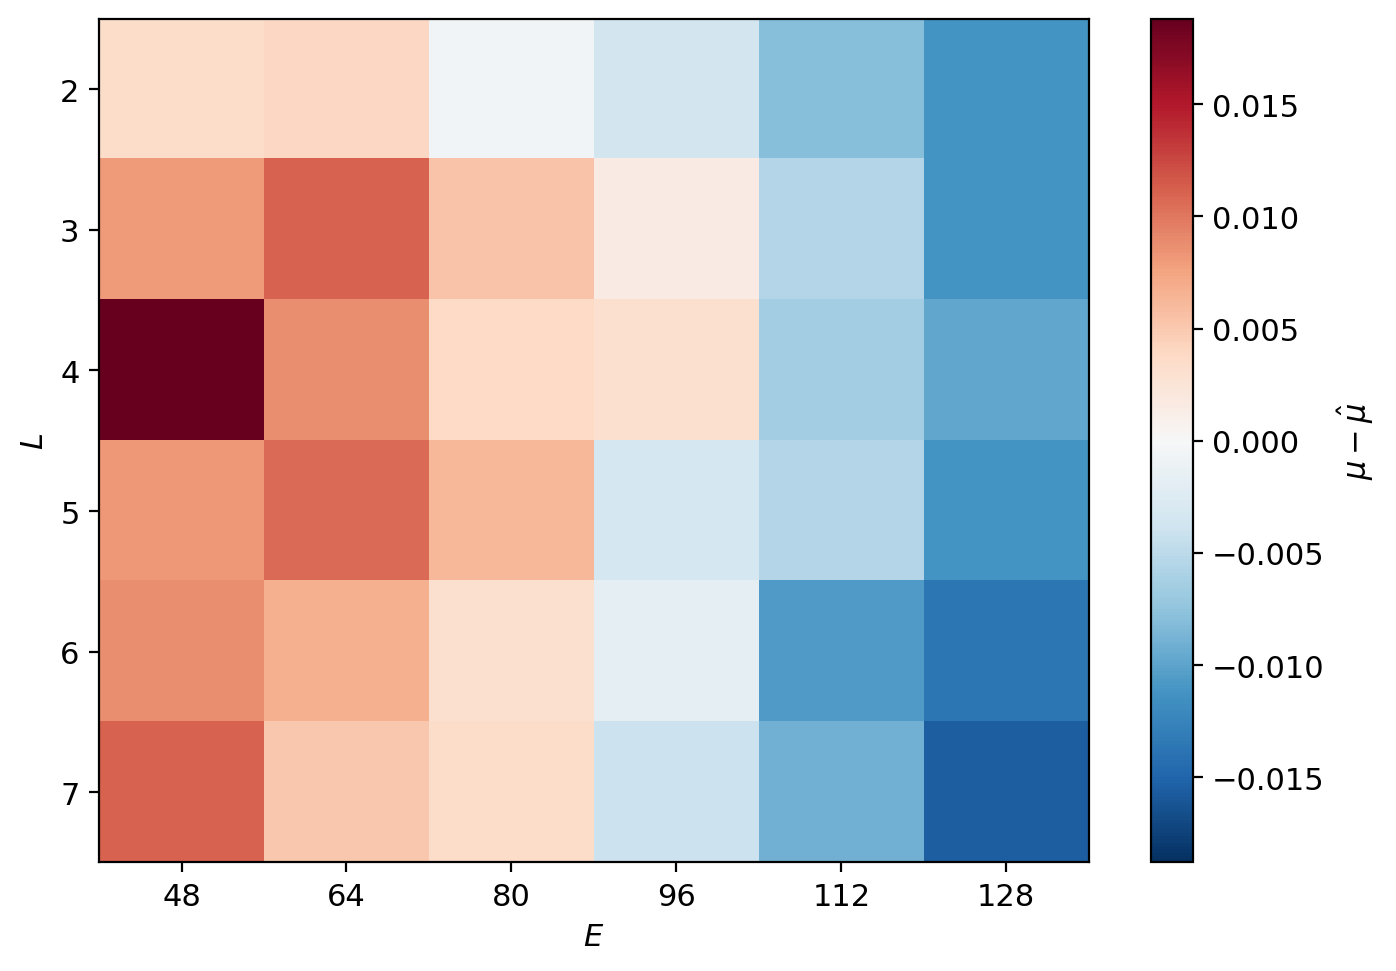
\includegraphics[height=0.17\textwidth]{thesis/figures/chapter-1/empirical-landscape/fig_grid_mu_residual_heatmap.png}
    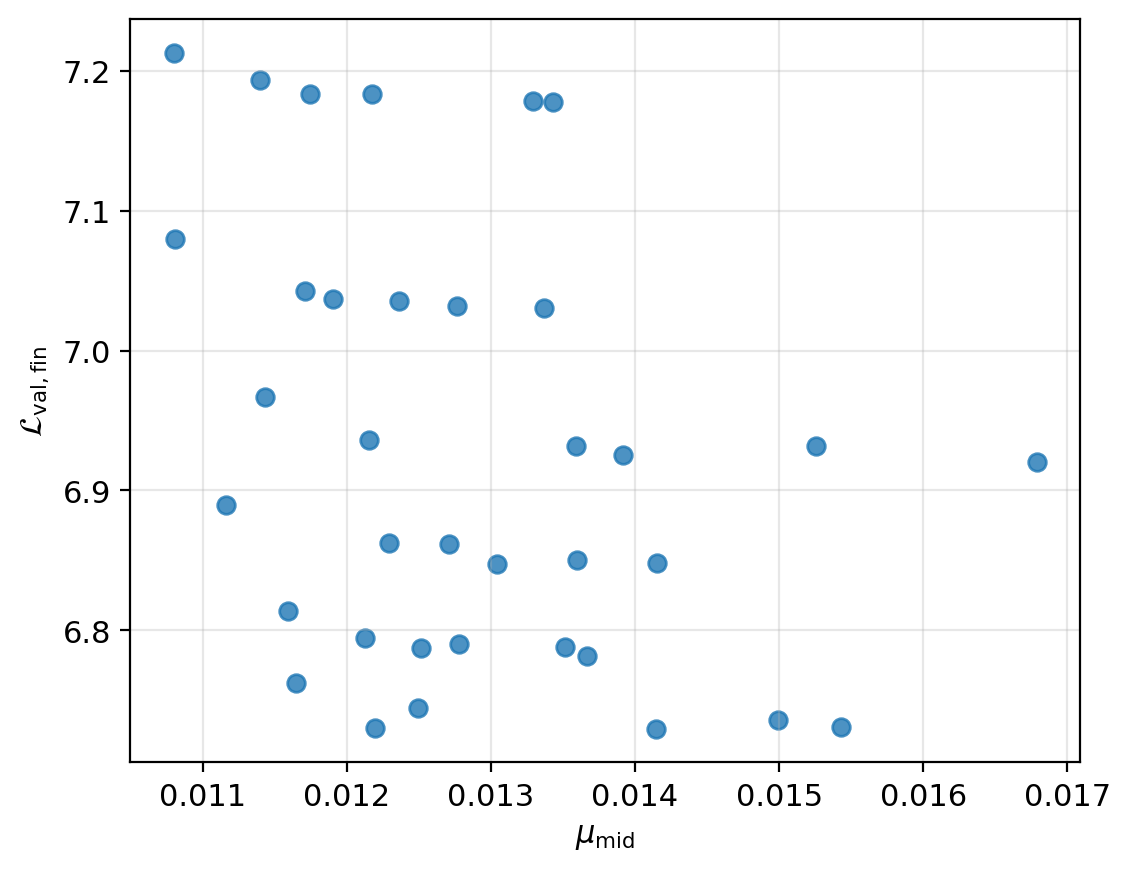
\includegraphics[height=0.17\textwidth]{thesis/figures/chapter-1/empirical-landscape/fig_mu_mid_vs_val_final.png}
\end{figure}
\key{Ландшафтная мера --- средняя спектральная норма отклонения пообъектной матрицы Гессе от средней по выборке.}
\end{frame}
%----------------------------------------------------------------------------------------------------------
\begin{frame}{Связь ландшафтной меры с приращением риска}
\justifying
\small
\setlength{\abovedisplayskip}{2pt}\setlength{\belowdisplayskip}{2pt}\setlength{\abovedisplayshortskip}{1pt}\setlength{\belowdisplayshortskip}{1pt}
При разложении Тейлора квадратичный член контролируется разностью матриц Гессе нового объекта и среднего:
\begin{align*}
    \bigl|\mathcal{L}_{k+1}(\boldsymbol{\theta})-\mathcal{L}_k(\boldsymbol{\theta})\bigr|
    &\le\frac{1}{k+1}\Bigl|\ell(f_{\boldsymbol{\theta}^*}(\mathbf{x}_{k+1}),\mathbf{y}_{k+1})-\frac{1}{k}\sum_{i=1}^{k}\ell(f_{\boldsymbol{\theta}^*}(\mathbf{x}_i),\mathbf{y}_i)\Bigr|\\
    &\quad+\frac{\|\boldsymbol{\theta}-\boldsymbol{\theta}^*\|_2^2}{2(k+1)}\Bigl\|\mathbf{H}_{k+1}(\boldsymbol{\theta}^*)-\frac{1}{k}\sum_{i=1}^{k}\mathbf{H}_i(\boldsymbol{\theta}^*)\Bigr\|_2
    +2\varepsilon_g\|\boldsymbol{\theta}-\boldsymbol{\theta}^*\|_2.
\end{align*}
Мажорируя $\bigl\|\mathbf{H}_{k+1}-k^{-1}\sum_{i=1}^{k}\mathbf{H}_{i}\bigr\|_2\le 2\bar\mu_f$, где $\bar\mu_f:=\max_i\bigl\|\mathbf{H}_{i}(\boldsymbol{\theta}^*)-\bar{\mathbf{H}}\bigr\|_2$ (в ожидании $\bar\mu_f\asymp\mu_f(f\mid D)$), получаем:
\[
    \bigl|\mathcal{L}_{k+1}(\boldsymbol{\theta})-\mathcal{L}_k(\boldsymbol{\theta})\bigr|
    \le \frac{2M_{\ell}}{k+1}+\frac{\bar\mu_f}{k+1}\bigl\|\boldsymbol{\theta}-\boldsymbol{\theta}^*\bigr\|_2^2.
\]
\begin{columns}[T]
\begin{column}{0.36\textwidth}
\begin{rusremark}
    При $\|\boldsymbol{\theta}-\boldsymbol{\theta}^*\|_2\le R$ и требовании $\bigl|\mathcal{L}_{k+1}-\mathcal{L}_k\bigr|\le\varepsilon$ получаем
    \[
        k+1 \ge \frac{2M_{\ell}+\bar\mu_f\,R^2}{\varepsilon}.
    \]
\end{rusremark}
\end{column}
\begin{column}{0.64\textwidth}
\begin{center}
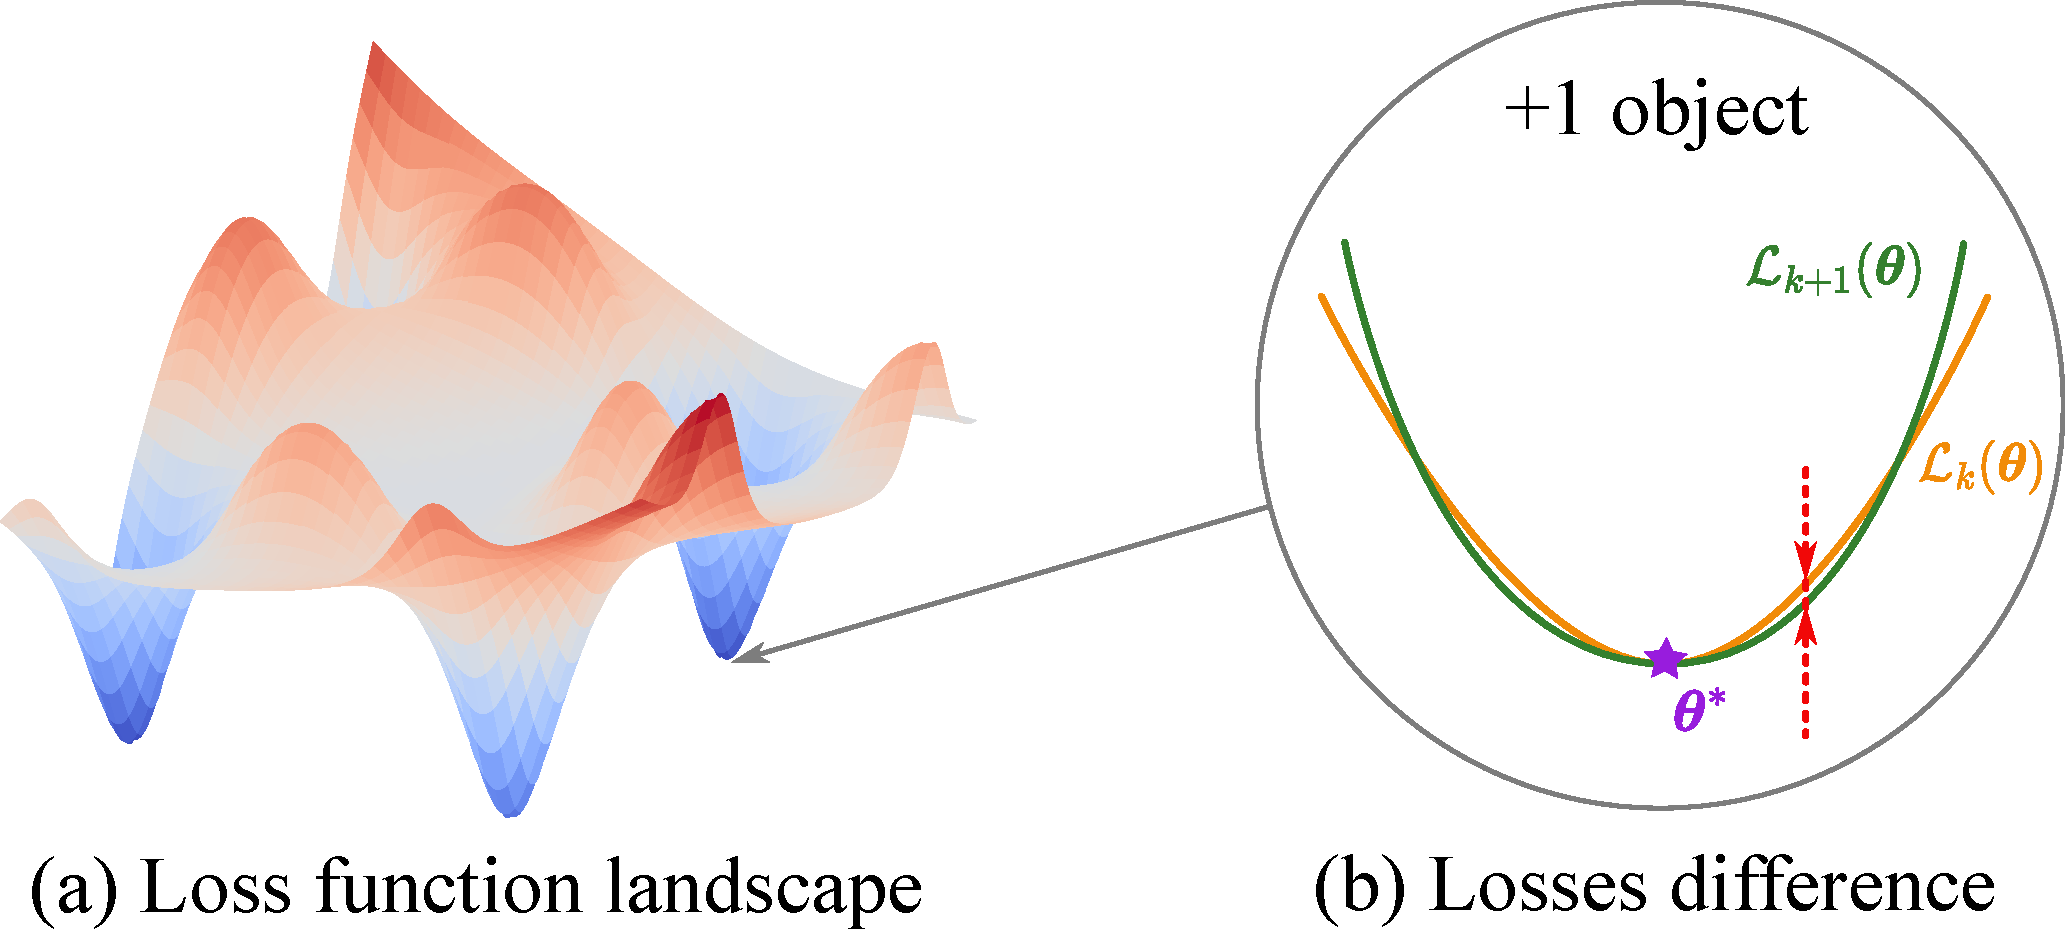
\includegraphics[height=0.18\textwidth]{thesis/figures/chapter-1/losses_difference.pdf}
\end{center}
\end{column}
\end{columns}

\key{Разброс матриц Гессе задает скорость стабилизации}
\end{frame}
%----------------------------------------------------------------------------------------------------------
\begin{frame}{Оценка скорости стабилизации эмпирического риска}
\justifying
\footnotesize
\begin{rustheorem}[Грабовой]
    Пусть заданы точка $\boldsymbol{\theta}^*$ и число $R>0$, и пусть выполнены следующие условия.
    \begin{enumerate}[1)]
        \item Для всех $i$ и всех $\boldsymbol{\theta}\in B_R(\boldsymbol{\theta}^*)$ функции $\ell(f_{\boldsymbol{\theta}}(\mathbf{x}_i),\mathbf{y}_i)$ имеют непрерывные третьи производные по $\boldsymbol{\theta}$.
        \item Существует константа $M_\ell\ge 0$ такая, что $\bigl|\ell(f_{\boldsymbol{\theta}^*}(\mathbf{x}_i),\mathbf{y}_i)\bigr|\le M_\ell$ для всех $i$.
        \item Существует константа $L_3\ge 0$ такая, что $\bigl\|\nabla^{3}_{\boldsymbol{\theta}}\ell(f_{\boldsymbol{\theta}}(\mathbf{x}_i),\mathbf{y}_i)\bigr\|_2\le L_3$ для всех $i$ и всех $\boldsymbol{\theta}\in B_R(\boldsymbol{\theta}^*)$.
        \item Выполнено предположение о приближенной стационарности с константой $\varepsilon_g\ge 0$.
        \item Радиус $R$ меньше расстояния от $\boldsymbol{\theta}^*$ до границы области, в которой функции $\ell(f_{\boldsymbol{\theta}}(\mathbf{x}_i),\mathbf{y}_i)$ трижды непрерывно дифференцируемы (в частности, до границы линейной области кусочно-линейной сети).
    \end{enumerate}
    Обозначим $\bar{\mathbf{H}}:=\mathbb{E}_{\mathbf{x}_i\in D}\mathbf{H}_{i}(\boldsymbol{\theta}^*)$ и $\bar\mu_f:=\max_i\bigl\|\mathbf{H}_{i}(\boldsymbol{\theta}^*)-\bar{\mathbf{H}}\bigr\|_2$, и пусть $A_1:=2M_\ell+\bar\mu_f R^2+L_3 R^3$. Тогда для любого $\boldsymbol{\theta}\in B_R(\boldsymbol{\theta}^*)$ и любого $k\ge 1$
    \[
        \bigl|\mathcal{L}_{k+1}(\boldsymbol{\theta})-\mathcal{L}_k(\boldsymbol{\theta})\bigr|
        \le \frac{A_1}{k+1}+2\,\varepsilon_g\,R .
    \]
\end{rustheorem}
\begin{rusremark}
    Оценка превращает стабилизацию ландшафта в количественное условие. Доминирующий вклад $\bar\mu_f R^2$ выражается через разброс матриц Гессе, входящий в ландшафтную меру: $\bar\mu_f\to\mu_f(f\mid D)$. Предположение о существовании единой стационарной точки $\boldsymbol{\theta}^*$ для всех $k$ является сильным упрощением: для невыпуклых функций потерь точка минимума сдвигается при добавлении объекта, поэтому оценка рассматривается как условная, а проверка условия --- численная.
\end{rusremark}
\key{Скорость стабилизации риска напрямую связана со сложностью модели.}
\end{frame}
%----------------------------------------------------------------------------------------------------------
\begin{frame}{Доказательство: стабилизация эмпирического риска}
\justifying
\footnotesize
\vspace{-2pt}
Источник скорости --- тождество скользящих средних:
\[
    \mathcal{L}_{k+1}-\mathcal{L}_k=\frac{1}{k+1}\bigl[\ell_{k+1}-\mathcal{L}_k\bigr].
\]
Тейлор по $\boldsymbol{\delta}=\boldsymbol{\theta}-\boldsymbol{\theta}^*$, $\|\boldsymbol{\delta}\|_2\le R$, в точке $\boldsymbol{\theta}^*$:
\[
    \frac{\ell_{k+1}-\mathcal{L}_k}{k+1}
    =\underbrace{\frac{\ell_{k+1}(\boldsymbol{\theta}^*)-\mathcal{L}_k(\boldsymbol{\theta}^*)}{k+1}}_{\text{(I)}}
    +\underbrace{\frac{\bigl(\nabla\ell_{k+1}(\boldsymbol{\theta}^*)-\nabla\mathcal{L}_k(\boldsymbol{\theta}^*)\bigr)^{\top}\boldsymbol{\delta}}{k+1}}_{\text{(II)}}
    +\underbrace{\frac{\tfrac12\boldsymbol{\delta}^{\top}\bigl(\mathbf{H}^{(k+1)}(\boldsymbol{\xi}_1)-\mathbf{H}^{(k)}(\boldsymbol{\xi}_2)\bigr)\boldsymbol{\delta}}{k+1}}_{\text{(III)}}.
\]
Покомпонентно:
\begin{itemize}
    \item (I): $\bigl|\ell_{k+1}(\boldsymbol{\theta}^*)-\mathcal{L}_k(\boldsymbol{\theta}^*)\bigr|\le 2M_\ell$;
    \item (II): $\bigl|(\nabla\ell_{k+1}(\boldsymbol{\theta}^*)-\nabla\mathcal{L}_k(\boldsymbol{\theta}^*))^{\top}\boldsymbol{\delta}\bigr|\le 2(k+1)\varepsilon_g R$;
    \item (III): $\bigl\|\mathbf{H}^{(k+1)}(\boldsymbol{\xi}_1)-\mathbf{H}^{(k)}(\boldsymbol{\xi}_2)\bigr\|_2\le 2\bar\mu_f+2L_3R$.
\end{itemize}
Складывая вклады, получаем
\[
    \bigl|\mathcal{L}_{k+1}-\mathcal{L}_k\bigr|\le\frac{2M_\ell+\bar\mu_fR^2+L_3R^3}{k+1}+2\varepsilon_gR=\frac{A_1}{k+1}+2\varepsilon_gR .
\]
\key{Источник $1/(k+1)$ --- тождество средних; доминирует (III) с разбросом гессианов $\bar\mu_f\to\mu_f(f\mid D)$, (I) ограничен $M_\ell$.}
\end{frame}
%----------------------------------------------------------------------------------------------------------
\begin{frame}{Оценка достаточного объема из стабилизации риска}
\justifying
\small
Если~$|\mathcal{L}_{k+1}-\mathcal{L}_k|\le\varepsilon$ при~$\|\boldsymbol{\theta}-\boldsymbol{\theta}^*\|_2\le R$, то из~$\frac{A_1}{k+1}+2\varepsilon_gR\le\varepsilon$ получаем
\[
    k+1\ge\frac{A_1}{\varepsilon-2\varepsilon_gR}=\frac{2M_\ell+\bar\mu_fR^2+L_3R^3}{\varepsilon-2\varepsilon_gR}.
\]
\begin{ruscorollary}
    \[
        k^\star=k^\star(\bar\mu_f,M_\ell,L_3,R,\varepsilon,\varepsilon_g),
    \]
    причем $k^\star$ растет с~$\bar\mu_f$, $M_\ell$, $L_3$ и~$R^2/\varepsilon$ при $\varepsilon_g=0$, при $\varepsilon_g>0$ зависимость от~$R$ и~$\varepsilon$ дробно-линейная. При $\varepsilon_g\to\varepsilon/2R$ знаменатель $\varepsilon-2\varepsilon_gR\to0$ и~$k^\star\to\infty$.
\end{ruscorollary}
\begin{rusremark}
    В ожидании по выборке допустима замена $\bar\mu_f\to\mu_f(f\mid D)$, поскольку $\mathbb{E}\|\mathbf{H}_{k+1}-\bar{\mathbf{H}}\|_2=\mu_f(f\mid D)$ и $\|\bar{\mathbf{H}}-\mathbf{H}^{(k)}\|_2=O(1/\sqrt{k})$. Условие $\bar\mu_f\asymp\mu_f(f\mid D)$ означает отсутствие выбросов и тяжелых хвостов в распределении норм матриц Гессе по объектам. При $\varepsilon_g>0$ правая часть содержит постоянное слагаемое $2\varepsilon_gR$, поэтому $\limsup_{k\to\infty}|\mathcal{L}_{k+1}-\mathcal{L}_k|\le 2\varepsilon_gR$.
\end{rusremark}
\key{Достаточный объем растет с разбросом матриц Гессе и обратно пропорционален точности аппроксимации.}
\end{frame}
%----------------------------------------------------------------------------------------------------------
\section{Меры сложности и критерий согласованности}
%----------------------------------------------------------------------------------------------------------
\begin{frame}{Меры сложности модели и выборки}
\justifying
\small
Ландшафтная мера $\mu_f(f\mid D)$ --- частный случай общей меры сложности модели.
\begin{rusdefinition}
    Мерой сложности модели~$f$ назовем отображение~$\mu_f:\mathfrak{F}\to\mathbb{R}_+$.
\end{rusdefinition}

\begin{rusdefinition}
    Мерой сложности выборки назовем отображение~$\mu_D:\mathfrak{D}_\Gamma\to\mathbb{R}_+$, удовлетворяющее для любых $D_i,D_j$ условию конечной субаддитивности
    \[
        \mu_D(D_i\cup D_j)\le\mu_D(D_i)+\mu_D(D_j),
    \]
    и условию монотонности по включению: $D_1\subseteq D_2\Rightarrow\mu_D(D_1)\le\mu_D(D_2)$. Аддитивность на непересекающихся множествах не предполагается.
\end{rusdefinition}

\begin{rusremark}
    Мера субаддитивна и монотонна, но не обязана быть аддитивной: сложность объединения может быть меньше суммы сложностей частей, например, за счет общих закономерностей, что позволяет учитывать сложность отдельных объектов, а не только мощность выборки.
\end{rusremark}
\key{Мера сложности модели --- характеристика, мера сложности выборки субаддитивна и монотонна.}
\end{frame}
%----------------------------------------------------------------------------------------------------------
\begin{frame}{Согласование модели и данных}
\justifying
\small
\begin{rusdefinition}
    Модель $f\in\mathfrak{F}$ назовем обучаемой на выборке $D\in\mathfrak{D}$, если
    \[
        \mu_f(f)\le\mu_D(D).
    \]
    Это условие согласования сложности модели и данных.
\end{rusdefinition}
\begin{rusproposition}
    Если $\mu_D$ монотонна по включению и $\mu_f(f)\le\mu_D(D)$, то для любой выборки $D'$ выполняется $\mu_f(f)\le\mu_D(D\cup D')$.
\end{rusproposition}
\begin{rusdefinition}
    Условной сложностью выборки назовем
    \[
        \mu_D(D\mid f)=\inf\bigl\{\mu_D(D'): D'\subseteq D,\; \mu_f(f)\le\mu_D(D')\bigr\},
    \]
    при этом $\inf\varnothing=+\infty$.
\end{rusdefinition}
\begin{rusremark}
    Условие $\mu_f(f)\le\mu_D(D)$ --- абстрактный критерий согласованности, а не критерий качества аппроксимации. Критерий носит порядковый характер и сравнивает сложность модели и выборки в едином масштабе. Конкретизация к достаточному размеру выборки задается выбором $\mu_D(D')=C\lvert D'\rvert$ с фиксацией $C=\varepsilon/R^2$.
\end{rusremark}
\key{Согласование: модель допустима, пока ее сложность не превосходит сложность данных. Ландшафтная мера зависит от решения $\boldsymbol{\theta}^*$ и выборки $D$.}
\end{frame}

%----------------------------------------------------------------------------------------------------------
\section{Оценки матриц Гессе для архитектур}
%----------------------------------------------------------------------------------------------------------
\begin{frame}{Декомпозиция матрицы Гессе}
\justifying
\small
\begin{rusdefinition}
    При $\mathbf{z}_i=f_{\boldsymbol{\theta}}(\mathbf{x}_i)\in\mathbb{R}^{K}$
    \[
        \mathbf{H}_i(\boldsymbol{\theta})=\underbrace{\nabla_{\boldsymbol{\theta}}\mathbf{z}_i\,\frac{\partial^2\ell(\mathbf{z}_i,\mathbf{y}_i)}{\partial\mathbf{z}_i^2}\,\nabla_{\boldsymbol{\theta}}\mathbf{z}_i^{\top}}_{\text{G-компонента}}+\underbrace{\sum_{k=1}^{K}\frac{\partial\ell(\mathbf{z}_i,\mathbf{y}_i)}{\partial z_{ik}}\nabla^2_{\boldsymbol{\theta}}z_{ik}}_{\text{H-компонента}}.
    \]
    $\nabla_{\boldsymbol{\theta}}\mathbf{z}_i$ --- матрица Якоби сети по параметрам, $\dfrac{\partial^2\ell}{\partial\mathbf{z}_i^2}$ --- Гессе потери по логитам. G-компонента отражает кривизну потери, H-компонента --- кривизну самой сети.
\end{rusdefinition}
\begin{rusremark}
    Спектральное распределение Гессе бимодально: основная масса собственных значений --- вблизи нуля, выбросы --- в области ненулевых значений. Для практического анализа релевантна G-компонента:
    $\mathbf{H}_{i}(\boldsymbol{\theta})\approx\nabla_{\boldsymbol{\theta}}\mathbf{z}_i\,\frac{\partial^2\ell(\mathbf{z}_i,\mathbf{y}_i)}{\partial\mathbf{z}_i^2}\,\nabla_{\boldsymbol{\theta}}\mathbf{z}_i^{\top}$.
\end{rusremark}
\key{Декомпозиция разделяет кривизну потери и кривизну отображения вход-выход, для анализа релевантна G-компонента.}
\end{frame}
%----------------------------------------------------------------------------------------------------------
\begin{frame}{Факторизация матричных моделей}
\justifying
\small
\begin{rusdefinition}
    Функция сети представима в виде
    \[
        f_{\boldsymbol{\theta}}(\mathbf{x}) = \mathbf{T}^{(L+1)}\boldsymbol{\Lambda}^{(L)}\dots \boldsymbol{\Lambda}^{(1)}\mathbf{T}^{(1)}\mathbf{x},
    \]
    где $\mathbf{T}^{(l)}$ --- матрицы линейных операторов, $\boldsymbol{\Lambda}^{(l)}=\mathrm{diag}(\mathbf{x}^{(l)}>0)$ --- бинарные маски активации. Сеть с активациями ReLU является кусочно-линейной функцией, нелинейность возникает за счет бинарных переключений в $\boldsymbol{\Lambda}^{(p)}$, при этом $\|\boldsymbol{\Lambda}^{(l)}\|_2\le1$.
\end{rusdefinition}
\begin{rustheorem}[Грабовой]
    Пусть функция нейронной сети $f_{\boldsymbol{\theta}}(\mathbf{x})$ представима в виде представления из определения, тогда матрица Гессе функции потерь относительно параметров модели может быть представлена в факторизованной форме
    \[
        \mathbf{H}_O(\boldsymbol{\theta})=\mathbf{Q}^{\top}\mathbf{F}^{\top}\mathbf{A}\mathbf{F}\mathbf{Q},
    \]
    где $\mathbf{H}_O$ описывает G-компоненту матрицы Гессе.
\end{rustheorem}
\begin{rusremark}
    $\mathbf{Q}^{(p)}=\partial\mathbf{T}^{(p)}/\partial\mathbf{W}^{(p)}$, $\mathbf{A}=\nabla^2_{\mathbf{z}}\ell=\mathrm{diag}(\mathbf{p})-\mathbf{p}\mathbf{p}^{\top}$ при кросс-энтропии.
\end{rusremark}
\key{Единая факторизация переносит оценку нормы Гессе на произвольную суперпозицию слоев с матрицами активации.}
\end{frame}
%----------------------------------------------------------------------------------------------------------
\begin{frame}{Доказательство: факторизация матрицы Гессе}
\justifying
\footnotesize
\vspace{-2pt}
Представление $f_{\boldsymbol{\theta}}(\mathbf{x})=\mathbf{T}^{(L+1)}\boldsymbol{\Lambda}^{(L)}\dots\boldsymbol{\Lambda}^{(1)}\mathbf{T}^{(1)}\mathbf{x}$, $\mathbf{Q}^{(p)}:=\partial\mathbf{T}^{(p)}/\partial\mathbf{W}^{(p)}$.
\begin{enumerate}[1)]
    \item \textbf{Идея.} Веса входят в $\mathbf{T}^{(p)}$ линейно $\Rightarrow$ кривизна порождается масками $\boldsymbol{\Lambda}^{(p)}$, а не весами. $\mathbf{H}_O$ расщепляется на маску $\mathbf{F}$ и веса $\mathbf{A}$, причем для ReLU $\mathbf{H}_O=0$ п.в.
    \item \textbf{Цепное правило.} $\dfrac{\partial\mathbf{z}}{\partial\mathbf{W}^{(p)}}=\bigl(\mathbf{G}^{(p)}\otimes\mathbf{x}^{(p-1)\top}\bigr)\mathbf{Q}^{(p)}$, по тождеству $\operatorname{vec}(\mathbf{B}\mathbf{V}\mathbf{A}^{\top})=(\mathbf{A}\otimes\mathbf{B})\operatorname{vec}(\mathbf{V})$.
    \item \textbf{Блоки Гессе.} $\mathbf{H}_O^{(kl)}=\mathbf{Q}^{(k)\top}\bigl(\mathbf{G}^{(k)\top}\otimes\mathbf{R}^{(k-1)}\mathbf{x}\bigr)\mathbf{A}\bigl(\mathbf{G}^{(l)}\otimes\mathbf{x}^{\top}\mathbf{R}^{(l-1)\top}\bigr)\mathbf{Q}^{(l)}$.
    \item \textbf{Сборка.} По всем слоям, $\mathbf{F}$ --- произведения Кронекера, $\mathbf{A}=\nabla^2_{\mathbf{z}}\ell$:
    \[
        \mathbf{H}_O=\mathbf{Q}^{\top}\mathbf{F}^{\top}\mathbf{A}\mathbf{F}\mathbf{Q}.
    \]
\end{enumerate}
\vspace{-2pt}
\key{Кривизна в масках $\Lambda$ (веса линейны) $\Rightarrow$ $\mathbf{H}_O=\mathbf{Q}^{\top}\mathbf{F}^{\top}\mathbf{A}\mathbf{F}\mathbf{Q}$, $\|\mathbf{H}_O\|\le\|\mathbf{Q}\|^2\|\mathbf{F}\|^2\|\mathbf{A}\|$.}
\end{frame}
%----------------------------------------------------------------------------------------------------------
\begin{frame}{Оценка нормы Гессе для полносвязных сетей}
\justifying
\small
\begin{rustheorem}[Киселев, Грабовой]
    Рассмотрим $L$-слойную полносвязную нейронную сеть с функцией активации ReLU и без членов смещения, применяемую для решения задачи классификации на $K$ классов. Предположим, что выполнены условия:
    \[
        \| \mathbf{W}^{(p)} \|_2 \leqslant M_{\mathbf{W}}, \qquad \| \mathbf{x}_i \|_2 \leqslant M_{\mathbf{x}},
    \]
    для всех слоев $p = 1, \ldots, L$ и для всех объектов $i = 1, \ldots, m$. Тогда для любого $i$ выполняется
    \[
        \left\| \mathbf{H}_i(\boldsymbol{\theta}) \right\|_2 \leqslant L \sqrt{2} M_{\mathbf{x}}^2 M_{\mathbf{W}}^{2L} + \sqrt{2} \dfrac{M_{\mathbf{W}}^2 (M_{\mathbf{W}}^{2L} - 1)}{M_{\mathbf{W}}^2 - 1}.
    \]
\end{rustheorem}
\begin{rusremark}
    Оценка записана при $\|\mathbf{W}^{(p)}\|_2=M_{\mathbf{W}}\neq1$ (при $M_{\mathbf{W}}=1$ второе слагаемое есть предел $\sqrt2 L$). Это частный случай факторизации $\mathbf{H}_O=\mathbf{Q}^{\top}\mathbf{F}^{\top}\mathbf{A}\mathbf{F}\mathbf{Q}$ для полносвязной параметризации и дает экспоненциальную зависимость от глубины $L$. Оценивается G-компонента $\mathbf{H}_O$: для кусочно-линейного ReLU вторая производная равна нулю почти всюду, поэтому H-компонента исчезает. Остаток Тейлора оценивается на отрезке $[\boldsymbol{\theta}^*,\boldsymbol{\theta}]$, не пересекающем границы линейных областей, внутри такой области сеть полиномиальна и третья производная конечна. При $|w_{ij}^{(p)}|\le M$ имеем $\|\mathbf{H}_i\|_2\lesssim L(hM)^{2L}$, то есть $\mu_f(f\mid D)\lesssim L(hM)^{2L}$.
\end{rusremark}
\key{Норма Гессе для полносвязной сети растет экспоненциально с глубиной.}
\end{frame}
%----------------------------------------------------------------------------------------------------------
\begin{frame}{Оценка нормы Гессе для сверточных сетей}
\justifying
\small
\begin{rustheorem}[Киселев, Мешков, Грабовой]
    Пусть задана сеть вида $f_{\boldsymbol{\theta}}(x) = C_{\mathbf{W}^{(L+1)}} \circ \sigma \circ \dots \circ \sigma \circ C_{\mathbf{W}^{(1)}}(x)$, где $C_{\mathbf{W}^{(i)}}$ --- одномерная свертка без дополнения и с единичным шагом. Пусть заданы оценки $C_l\le C$, $k_l\le k_{\mathrm{ker}}$, $d_l\le d$, $|\mathbf{W}^{(l)}_{i,j,k}|^2\le w^2$. Тогда
    \[
        \left\|\mathbf{H}_{O}\right\| \leqslant \sqrt{2}\left\|x\right\|^2d^2(L+1)(C^2w^2k_{\mathrm{ker}}d)^L.
    \]
    Для двумерной свертки $f_{\boldsymbol{\theta}}\mathbf{x} = C_{\mathbf{W}^{(L+1)}} \circ \dots \circ C_{\mathbf{W}^{(1)}}$ при $C_l\le C$, $k_l\le k_{\mathrm{ker}}$, $m_l\le m$, $n_l\le n$, $|\mathbf{W}^{(l)}_{i,j,k}|^2\le w^2$ и $q^2=C^2k_{\mathrm{ker}}^2mn$ справедливо
    \[
        \left\|\mathbf{H}_{O}\right\| \leqslant \sqrt{2}\left\|\mathbf{x}\right\|^2q^2(L+1)(C^2k_{\mathrm{ker}}^2w^2mn)^{L}.
    \]
\end{rustheorem}
\begin{rusremark}
    Оценки являются частным случаем теоремы о факторизации $\mathbf{H}_O=\mathbf{Q}^{\top}\mathbf{F}^{\top}\mathbf{A}\mathbf{F}\mathbf{Q}$ для сверточной параметризации. Оценивается G-компонента $\mathbf{H}_O$: для кусочно-линейного ReLU вторая производная равна нулю почти всюду, поэтому H-компонента исчезает, а формулы рассматриваются на дополнении к аффинному множеству нулей предактиваций (что не меняет вид спектральных мажорант). Остаток Тейлора оценивается на отрезке $[\boldsymbol{\theta}^*,\boldsymbol{\theta}]$, не пересекающем границы линейных областей, то есть при $R$ меньше расстояния от $\boldsymbol{\theta}^*$ до границы линейной области, внутри такой области сеть полиномиальна и третья производная конечна.
\end{rusremark}
\key{Норма Гессе для сверточных сетей: экспонента по глубине, полином по каналам и размеру ядра.}
\end{frame}
%----------------------------------------------------------------------------------------------------------
\begin{frame}{Сверточные сети: каналы, размер ядра и пулинг}
\justifying
\small
\begin{center}
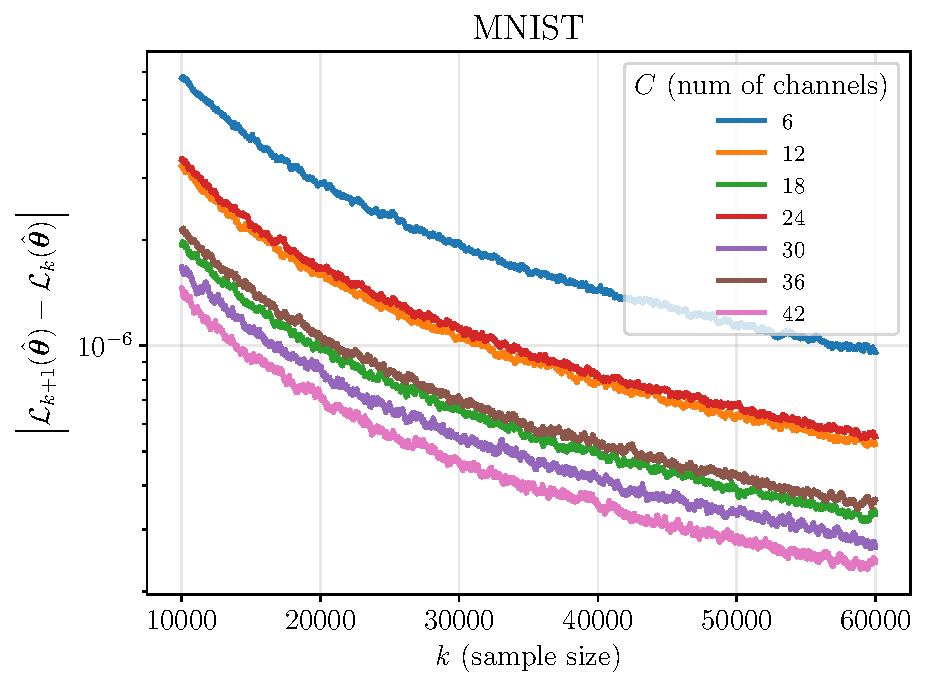
\includegraphics[width=0.49\textwidth]{thesis/figures/chapter-1/matricized-networks/mnist_change_channels.pdf}\hfill
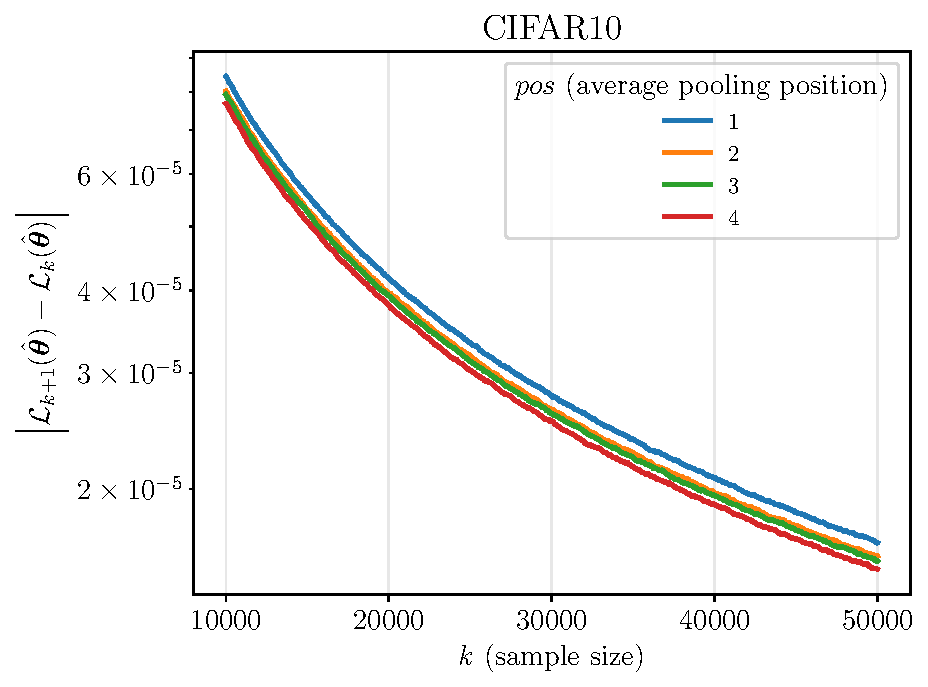
\includegraphics[width=0.49\textwidth]{thesis/figures/chapter-1/matricized-networks/cifar10_change_avgpool_pos.pdf}
\end{center}
\vspace{2pt}
\begin{itemize}
    \setlength{\itemsep}{2pt}
    \item Изменение числа каналов $C$ и размера ядра свертки $k$ дает нелинейный отклик разности потерь $|\mathcal{L}_{k+1}-\mathcal{L}_k|$.
    \item Положение усредняющего пулинга меняет скорость сходимости ландшафта: ранний пулинг снижает разность потерь.
\end{itemize}
\key{Сверточные параметры влияют на ландшафт через число каналов и позицию пулинга.}
\end{frame}
%----------------------------------------------------------------------------------------------------------
\begin{frame}{Оценка нормы Гессе для слоя самовнимания}
\justifying
\small
\begin{rustheorem}[Грабовой]
    Пусть $\|\cdot\|_2$ является спектральной нормой, тогда для слоя самовнимания
    \[
        \|\mathbf{H}_i(\mathbf{w}^*)\|_2 \leq M,
    \]
    где
    \[
    \resizebox{\textwidth}{!}{$\begin{aligned}
    M &= 3\cdot\max \Big(\frac{2N}{d_V} \| \mathbf{X}\|^2_2, \\
        &\frac{8}{N^3 d_V d_K} \| \mathbf{W}_K\|_2^2 \| \mathbf{W}_V\|^2_2 \| \mathbf{X}\|^6_2 + \frac{12}{d_V d_K} \sqrt{\min(N, d_V)} (N \|\mathbf{X}\|_2 \|\mathbf{W}_V \|_2 + \|\textbf{Target}\|_2) \| \mathbf{W}_V \|_2 \| \mathbf{W}_K\|^2_2 \| \mathbf{X}\|^5_2, \\
        &\frac{4}{N d_V \sqrt{d_K}} \| \mathbf{W}_V\|_2 \| \mathbf{W}_K \|_2 \| \mathbf{X}\|^4_2 + \frac{4\sqrt{\min(N, d_V)}}{N^2\sqrt{d_K}} (N \|\mathbf{X}\|_2 \|\mathbf{W}_V \|_2 + \|\textbf{Target}\|_2) \|\mathbf{W}_K\|_2 \|\mathbf{X}\|^3_2, \\
        &\frac{8}{N^3 d_V d_K} \|\mathbf{W}_K\|_2 \|\mathbf{W}_Q\|_2 \| \mathbf{W}_V\|^2_2 \|\mathbf{X} \|^6_2 + \frac{4\sqrt{\min(N, d_V)} (N \|\mathbf{X}\|_2 \|\mathbf{W}_V \|_2 + \|\textbf{Target}\|_2)}{N d_V \sqrt{d_K}} \|\mathbf{W}_V\|_2 \cdot\\
        &\quad\cdot\Big(3N \|\mathbf{W}_K\|_2 \|\mathbf{W}_Q\|_2 \| \mathbf{X}\|^5_2 + \frac{d_V}{N} \|\mathbf{X}\|^3_2\Big)\Big).
    \end{aligned}$}
    \]
\end{rustheorem}
\begin{rusremark}
    Величина $M$ задается максимумом из трех слагаемых. Первое зависит только от $N/d_V$ и $\|\mathbf{X}\|_2$; второе и третье растут с нормами весовых матриц $\mathbf{W}_K,\mathbf{W}_V,\mathbf{W}_Q$ и размерностями $d_K,d_V$. По входу слагаемые пропорциональны $\|\mathbf{X}\|_2^3,\ldots,\|\mathbf{X}\|_2^6$. Здесь ограничивается один слой самовнимания.
\end{rusremark}
\key{Норма Гессе слоя самовнимания растет с нормой входа $\|\mathbf{X}\|_2$ и нормами весовых матриц $\mathbf{W}$; вклад по входу --- до $\|\mathbf{X}\|_2^6$.}
\end{frame}
%----------------------------------------------------------------------------------------------------------
%----------------------------------------------------------------------------------------------------------
\begin{frame}{Норма Гессе в трансформере: как выглядит оценка}
\justifying
\small
\begin{center}
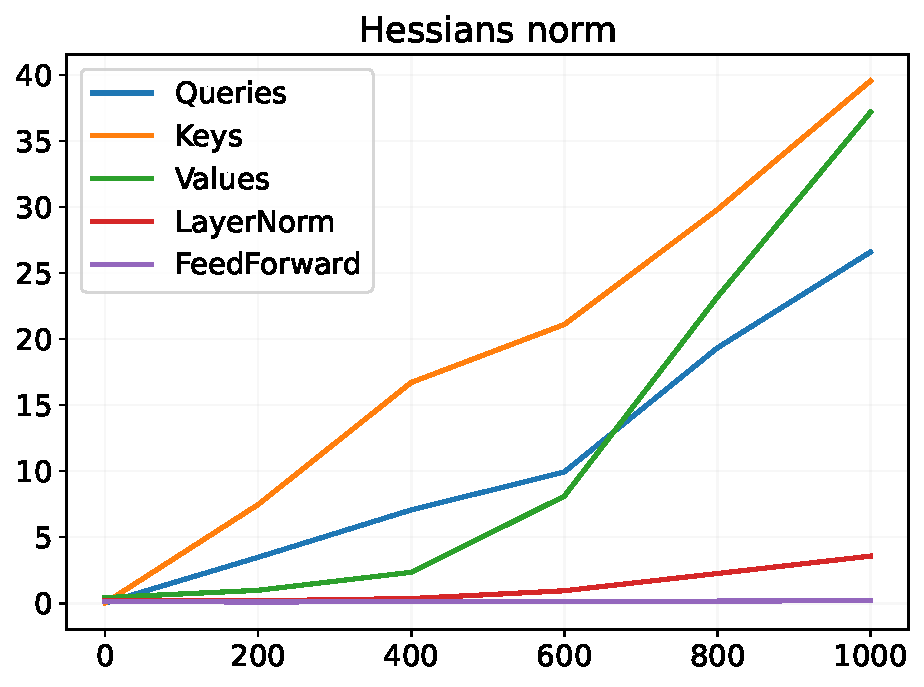
\includegraphics[width=0.45\textwidth]{thesis/figures/chapter-2/transformer/hessians_norm.pdf}\hfill
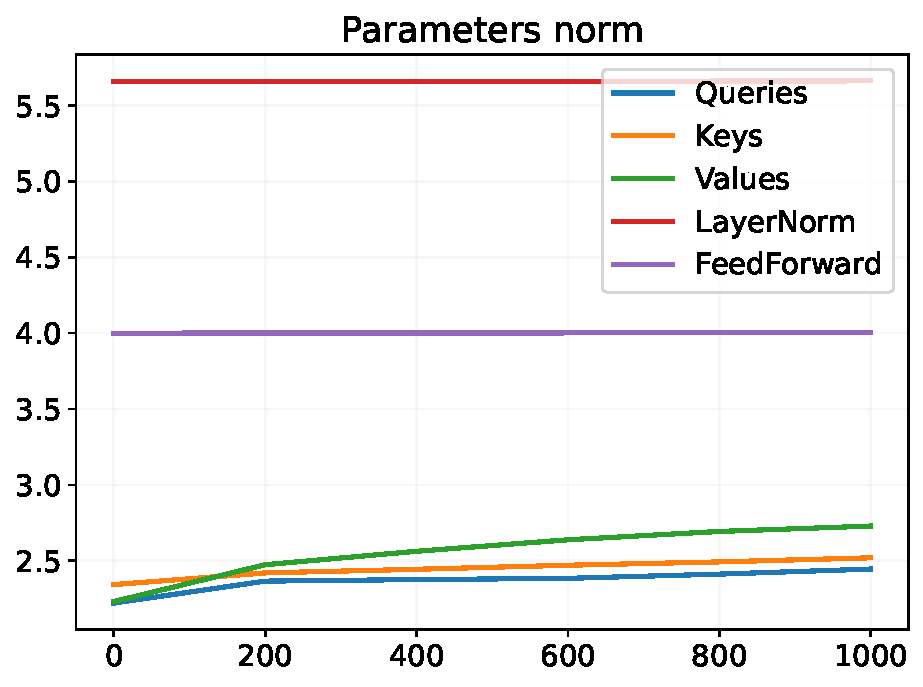
\includegraphics[width=0.45\textwidth]{thesis/figures/chapter-2/transformer/parameters_norm.pdf}
\end{center}
\vspace{2pt}
\begin{itemize}
    \setlength{\itemsep}{2pt}
    \item Нормы матриц Гессе по компонентам трансформера (keys/queries/values/feed-forward) соотносятся со слагаемыми оценки $M$.
    \item Рост нормы Гессе следует за ростом нормы параметров.
\end{itemize}
\key{Оценка нормы Гессе для самовнимания согласуется с наблюдаемыми нормами по компонентам.}
\end{frame}
%----------------------------------------------------------------------------------------------------------
\begin{frame}{Связь норм Гессе и ландшафтной меры}
\justifying
\small
\begin{rusdefinition}
    По определению $\mu_f(f\mid D)=\mathbb{E}_{\mathbf{x}_i\in D}\bigl\|\mathbf{H}_{i}(\boldsymbol{\theta}^*)-\mathbb{E}_{\mathbf{x}_i\in D}\mathbf{H}_{i}(\boldsymbol{\theta}^*)\bigr\|_2$ и неравенству треугольника
    \[
        \mu_f(f\mid D)\le\max_i\bigl\|\mathbf{H}_{i}(\boldsymbol{\theta}^*)-\bar{\mathbf{H}}\bigr\|_2\le 2\sup_i\bigl\|\mathbf{H}_{i}(\boldsymbol{\theta}^*)\bigr\|_2\le 2B,
    \]
    где $\bar{\mathbf{H}}=\mathbb{E}_{\mathbf{x}_i\in D}\mathbf{H}_{i}(\boldsymbol{\theta}^*)$ и $B:=\sup_i\|\mathbf{H}_{i}(\boldsymbol{\theta}^*)\|_2$. Усреднение по $i$ не превосходит максимума, а $\|\mathbf{H}_i-\bar{\mathbf{H}}\|_2\le\|\mathbf{H}_i\|_2+\|\bar{\mathbf{H}}\|_2\le 2\sup_i\|\mathbf{H}_i\|_2$.
\end{rusdefinition}
\begin{rusremark}
    Оценка $\|\mathbf{H}_i\|_2\le B$ влечет $\mu_f(f\mid D)\le 2B$. Тем самым спектральные оценки норм Гессе дают вычислимую мажоранту ландшафтной меры сложности.
\end{rusremark}
\begin{block}{Порядки мажоранты $\mu_f(f\mid D)$ (при $\|\mathbf{H}_i\|_2\le B$)}
\footnotesize
\begin{tabular}{|l|c|l|}
\hline
\textbf{Архитектура} & \textbf{Оцениваемая норма} & \textbf{Порядок мажоранты} \\
\hline
Полносвязная & $\|\mathbf{H}_i\|_2$ & $O\bigl(L(hM)^{2L}\bigr)$ \\
\hline
1D-сверточная & $\|\mathbf{H}_O\|_2$ & $O\bigl(L(C^2w^2k_{\mathrm{ker}}d)^L\bigr)$ \\
\hline
2D-сверточная & $\|\mathbf{H}_O\|_2$ & $O\bigl(L(C^2k_{\mathrm{ker}}^2w^2mn)^L\bigr)$ \\
\hline
Слой самовнимания & $\|\mathbf{H}_i\|_2$ & максимум разнородных слагаемых \\
\hline
\end{tabular}
\end{block}
\key{Оценка нормы Гессе дает вычислимую мажоранту $\mu_f(f\mid D)\le 2\sup_i\|\mathbf{H}_i\|_2$.}
\end{frame}
%----------------------------------------------------------------------------------------------------------
\begin{frame}{Спектр Гессе и ландшафтная мера}
\justifying
\small
\begin{center}
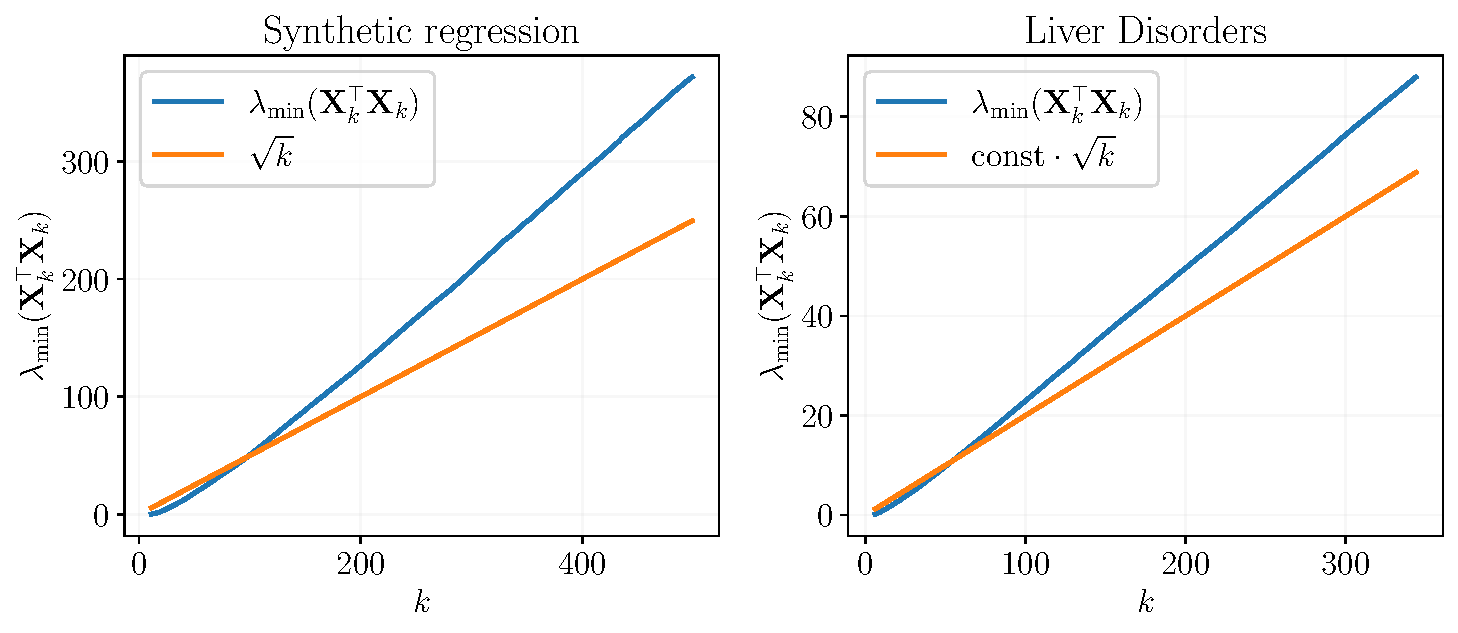
\includegraphics[width=0.62\textwidth]{thesis/figures/chapter-3/posterior-distribution/eigvals.pdf}
\end{center}
\vspace{2pt}
\begin{itemize}
    \setlength{\itemsep}{2pt}
    \item В обученном минимуме большинство собственных значений матрицы Гессе сосредоточено около нуля, и лишь единичные направления имеют заметную кривизну.
    \item Разброс пообъектных матриц Гессе относительно среднего и фиксирует ландшафтная мера $\mu_f(f\mid D)$.
\end{itemize}
\key{Спектр Гессе показывает избыточность параметров, а ландшафтная мера ловит их разброс по объектам.}
\end{frame}
%----------------------------------------------------------------------------------------------------------
\begin{frame}{Экспериментальная проверка ландшафтных оценок}
\justifying
\small
\begin{figure}[h!t]\center
\begin{minipage}[t]{0.32\textwidth}
\centering
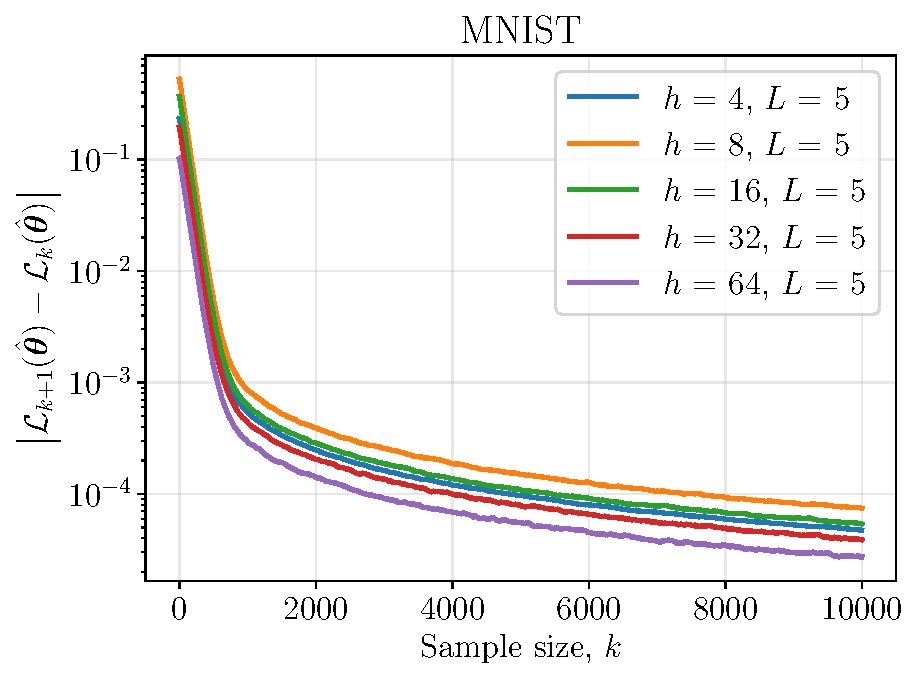
\includegraphics[width=\linewidth]{thesis/figures/chapter-1/landscape-hessian/figs/mnist_hidden_size.pdf}\\
{\footnotesize MNIST, $L=5$, $h$ от $4$ до $64$.}
\end{minipage}\hfill
\begin{minipage}[t]{0.32\textwidth}
\centering
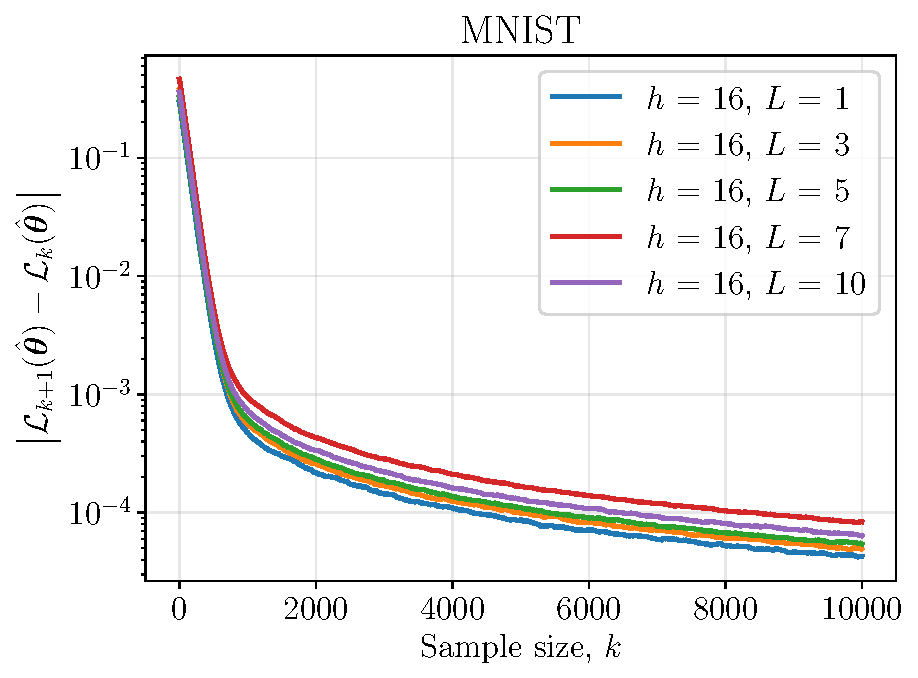
\includegraphics[width=\linewidth]{thesis/figures/chapter-1/landscape-hessian/figs/mnist_num_layers.pdf}\\
{\footnotesize MNIST, $h=16$, $L$ от $1$ до $10$.}
\end{minipage}\hfill
\begin{minipage}[t]{0.32\textwidth}
\centering
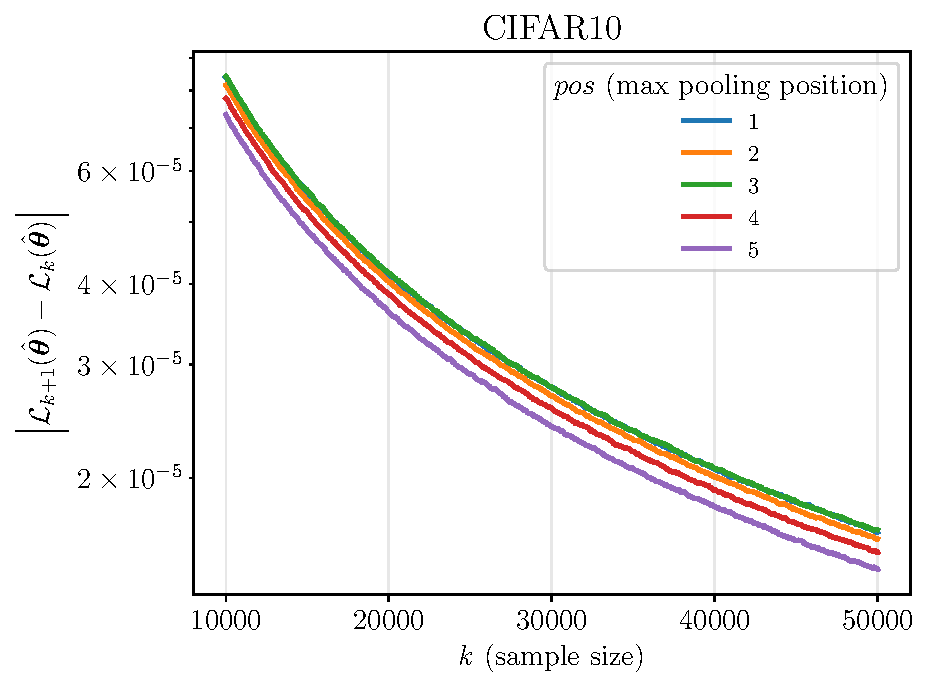
\includegraphics[width=\linewidth]{thesis/figures/chapter-1/matricized-networks/cifar10_change_maxpool_pos.pdf}\\
{\footnotesize CIFAR10, позиция пулинга.}
\end{minipage}
\end{figure}
\smallskip
\begin{itemize}
    \setlength{\itemsep}{2pt}
    \item Монотонное убывание разности потерь $|\mathcal{L}_{k+1}-\mathcal{L}_k|$ подтверждено на MNIST, FashionMNIST, CIFAR10.
    \item Увеличение глубины $L$ дает более медленную сходимость.
    \item Увеличение ширины $h$ влияет слабее --- согласуется с $\mu_f(f\mid D)\lesssim L(hM)^{2L}$.
    \item Ранний пулинг снижает разность потерь.
\end{itemize}
\key{Эксперименты подтверждают асимптотический характер оценок ландшафтной меры.}
\end{frame}
%----------------------------------------------------------------------------------------------------------
\begin{frame}{Сходимость ландшафта при признаковом экстракторе (ViT)}
\justifying
\small
\begin{center}
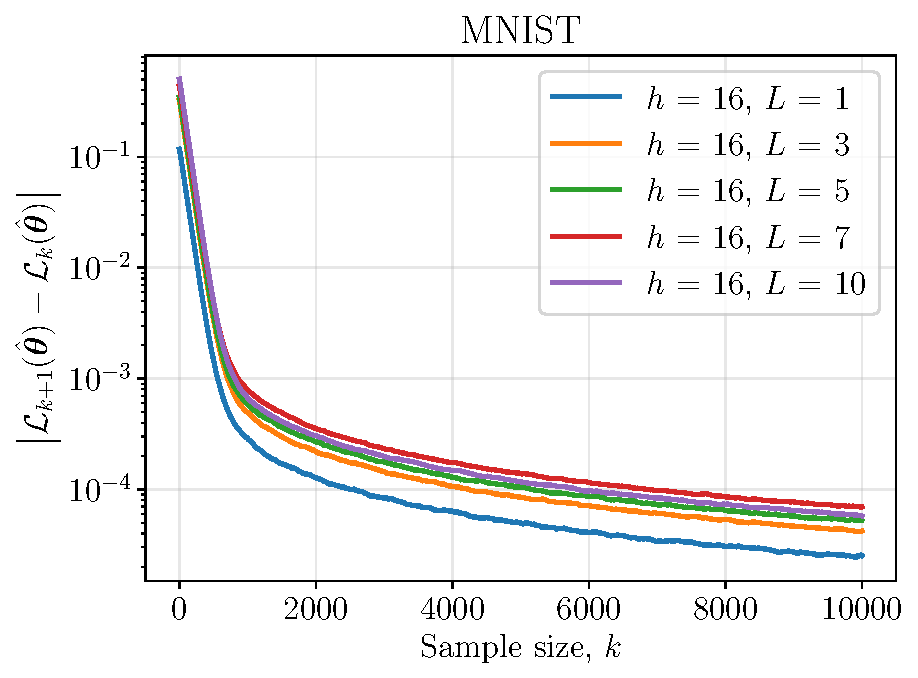
\includegraphics[width=0.49\textwidth]{thesis/figures/chapter-1/landscape-hessian/figs_extraction/mnist_num_layers.pdf}\hfill
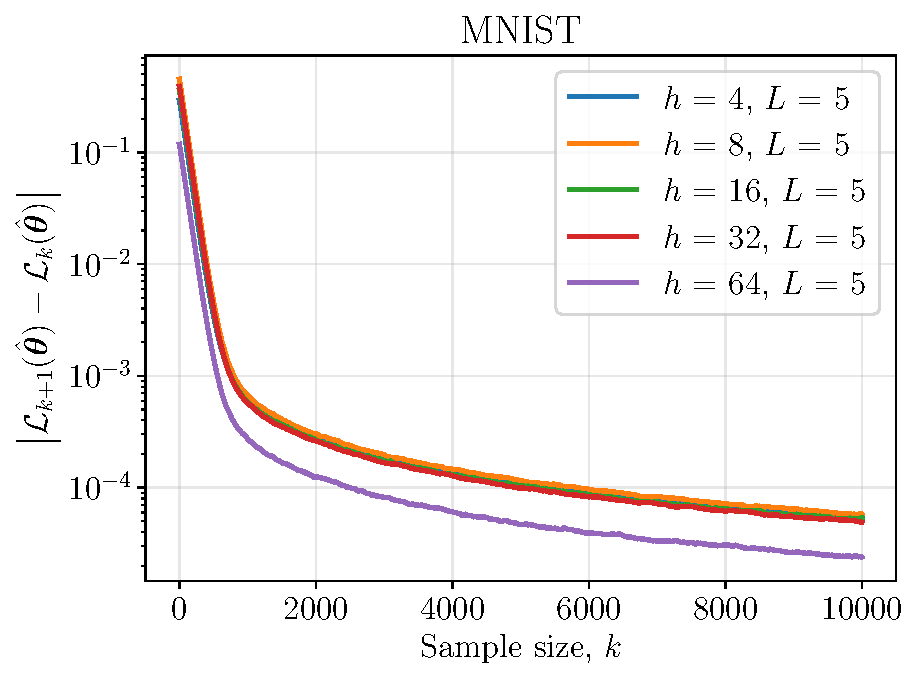
\includegraphics[width=0.49\textwidth]{thesis/figures/chapter-1/landscape-hessian/figs_extraction/mnist_hidden_size.pdf}
\end{center}
\vspace{2pt}
Зависимость $\bigl|\mathcal{L}_{k+1}(\boldsymbol{\theta})-\mathcal{L}_k(\boldsymbol{\theta})\bigr|$ от размера выборки $k$ для полносвязной сети на MNIST, когда вход сети --- признаки предобученного энкодера вместо сырых пикселей.
\begin{itemize}
    \setlength{\itemsep}{2pt}
    \item Справа: при $h=16$ разность растет с глубиной $L$ от $1$ до $10$.
    \item Слева: при $L=5$ разность убывает с шириной $h$ от $4$ до $64$.
\end{itemize}
\key{Тот же характер зависимостей от $L$ и $h$ сохраняется при входе в виде признаков предобученного экстрактора, что согласуется с теоремой о сходимости ландшафта.}
\end{frame}
%----------------------------------------------------------------------------------------------------------
\begin{frame}{Ландшафтная мера и радемахеровская сложность}
\small
\centering
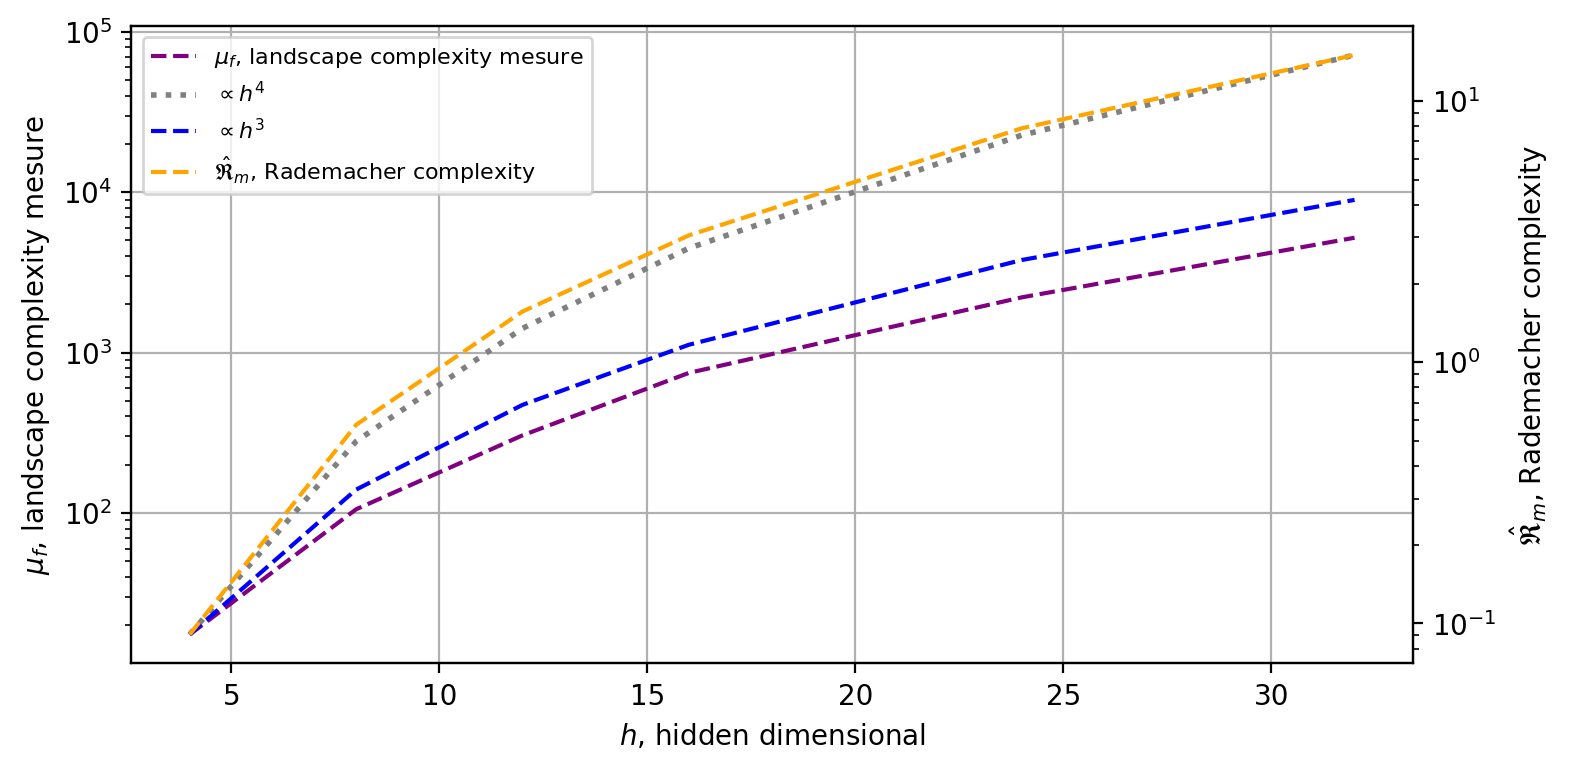
\includegraphics[width=0.70\textwidth]{thesis/figures/chapter-1/landscape-comparison/exp03_twolayer_sweep_h.png}\\[2pt]
{\footnotesize Двухслойная FC ReLU-сеть: $n=h$, $M=1$, $m=512$, $h\in\{4,8,12,16,24,32\}$.}
\vspace{2pt}
\raggedright
\smallskip
\begin{itemize}
    \setlength{\itemsep}{2pt}
    \item Оценка $\mu_f(f\mid D)$ по батчам пообъектных матриц Гессе (блок $64$), $\hat{\mathfrak{R}}_m$ покоординатным PGD ($n_\sigma=64$ шага).
    \item Опорные кривые, нормированные по наименьшему $h$: $\propto(Mh)^4$ (худший случай) и $\propto h^3$ (GN при $n=h$, с учетом малых остатков).
    \item Оценка худшего случая завышена: при малых остатках рост по ширине смягчается до $\mu_f(f\mid D)\sim h^3$.
\end{itemize}
\key{Малые остатки смягчают рост по ширине с $O((hM)^4)$ до~$\mu_f(f\mid D)\sim h^3$.}
\end{frame}
%----------------------------------------------------------------------------------------------------------
\begin{frame}{Динамика ландшафтной меры языковых моделей}
\justifying
\small
{\footnotesize Семейство GPT-2, корпус WikiText-103. Сетка $(L,H,E)$: $L\in\{2,\dots,7\}$, $H\in\{2,4\}$, $E\in\{48,\dots,128\}$ --- $36$ конфигураций. Бюджет $\approx 1{,}2\cdot 10^{7}$ токенов, $20$ контрольных точек, мини-пакет $128$, $8$ независимых запусков, AdamW.}
\vspace{2pt}
\begin{figure}[t]\center
\begin{minipage}[t]{0.30\textwidth}\centering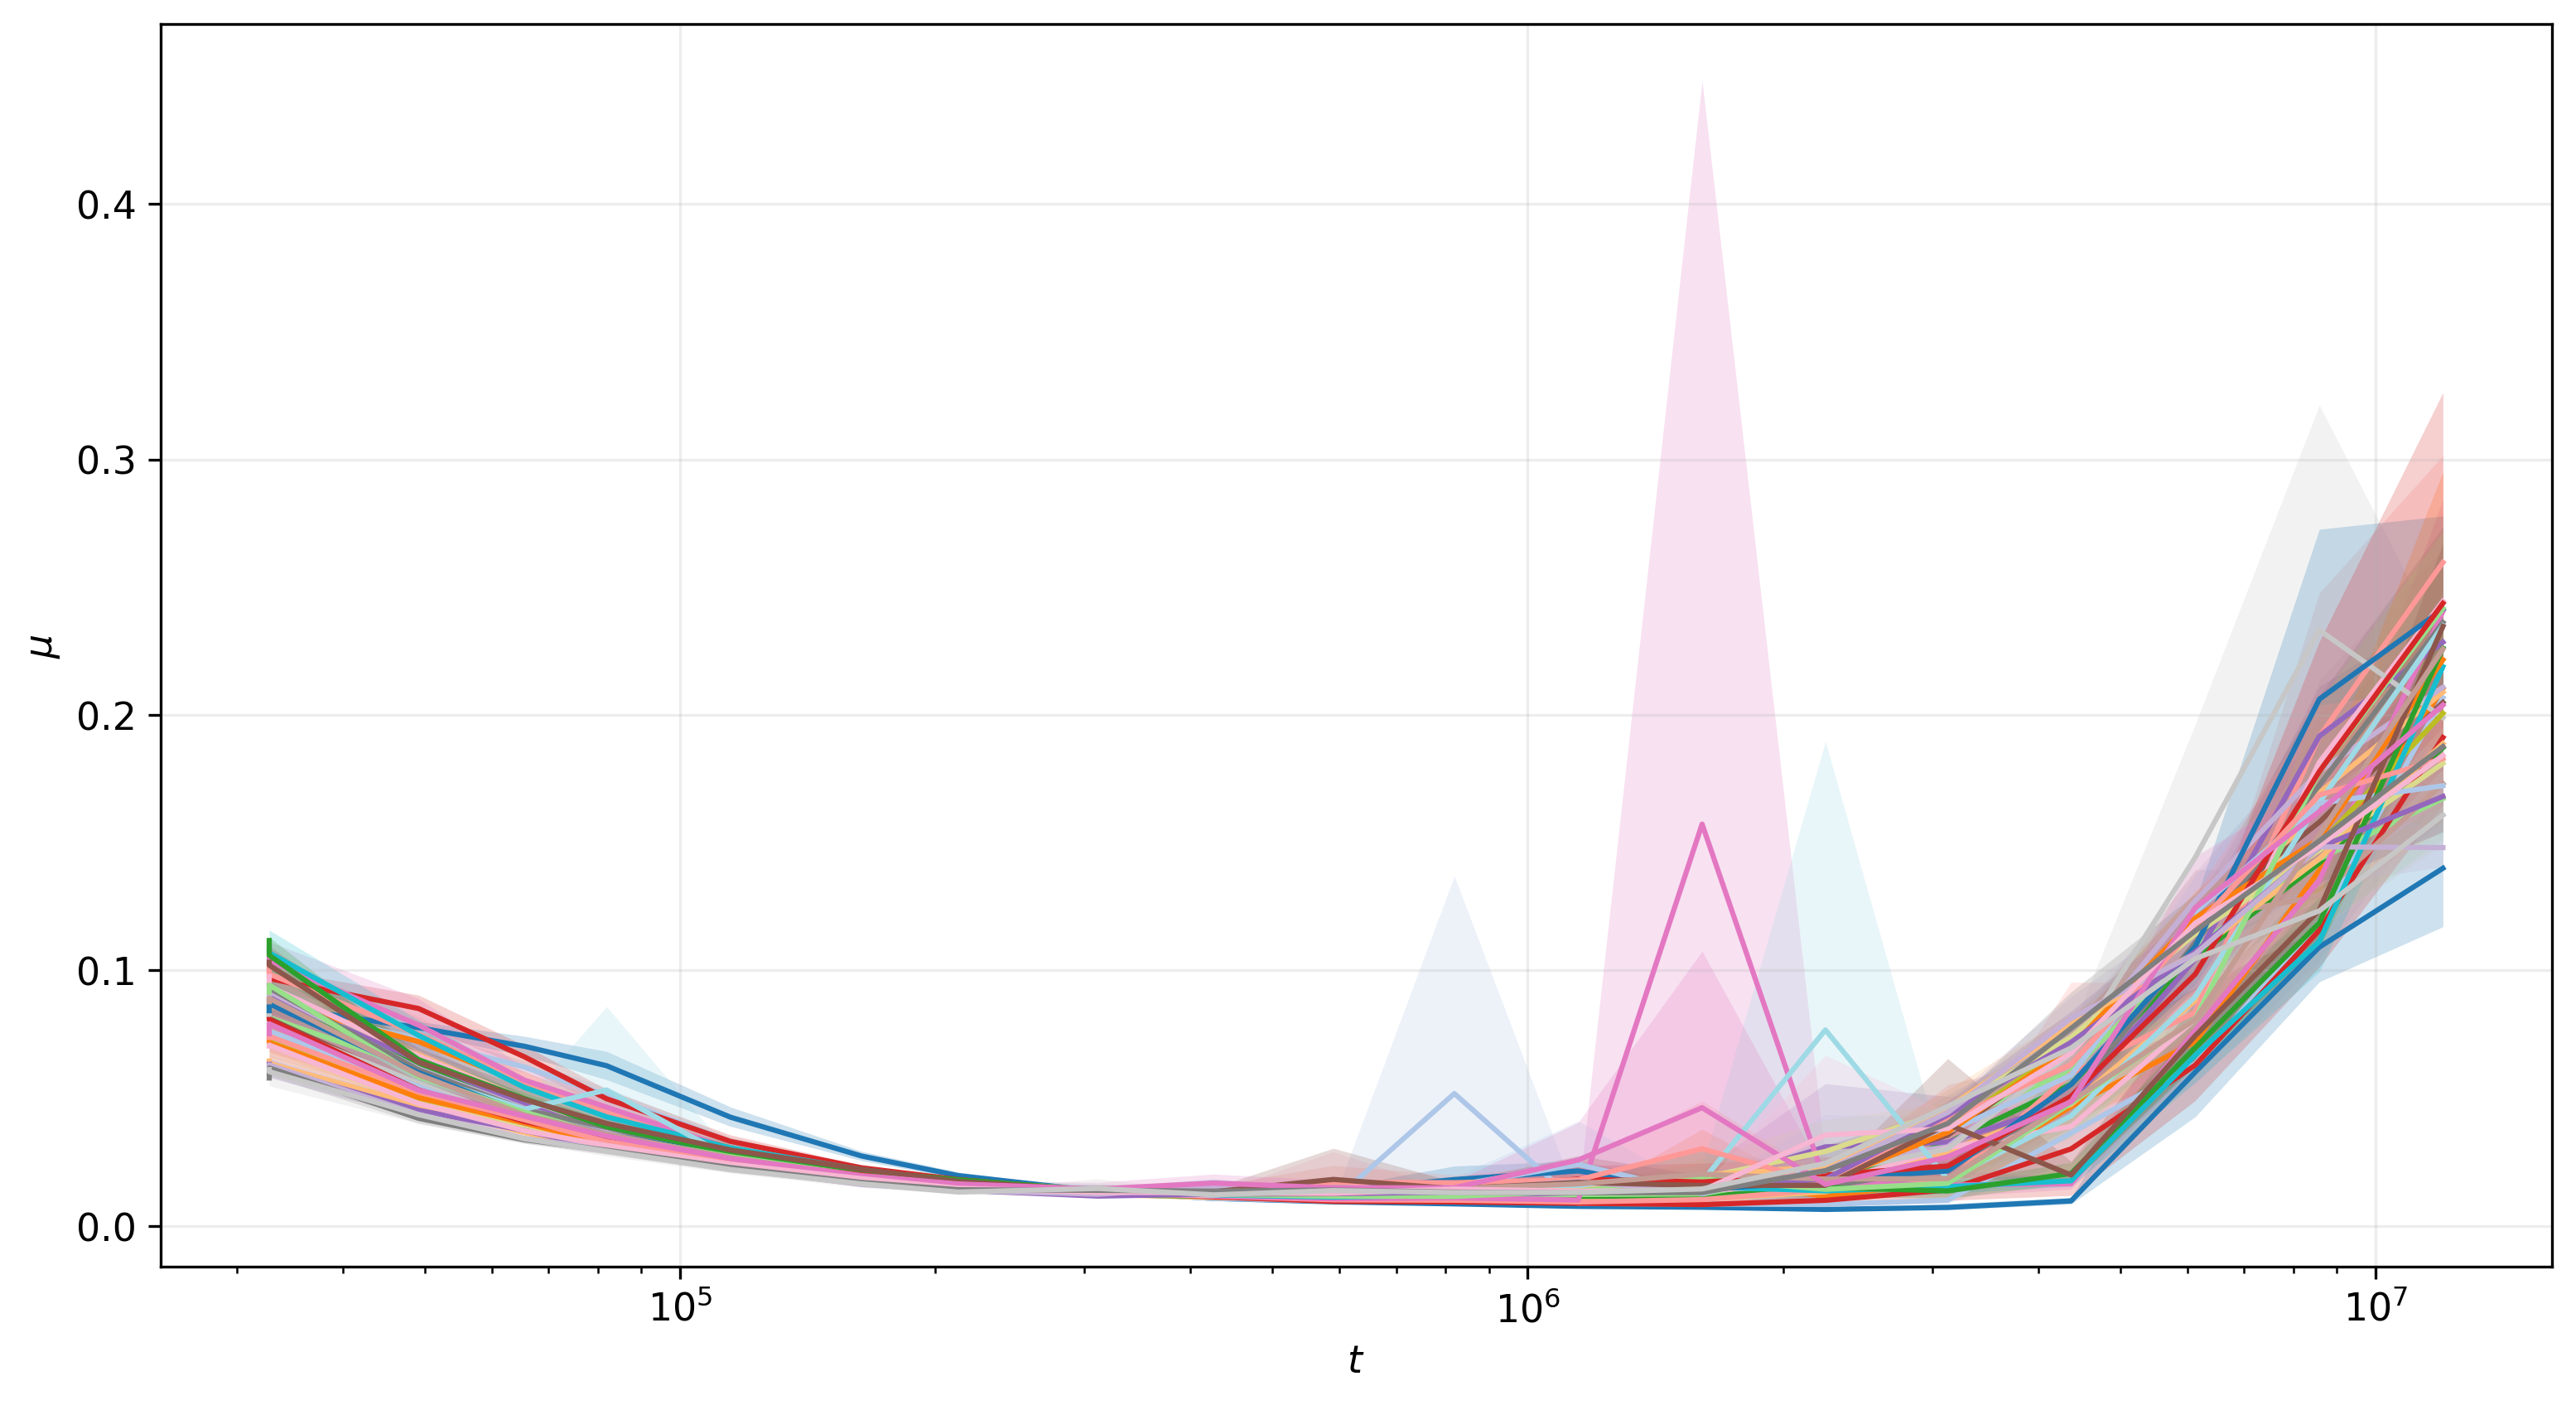
\includegraphics[width=\linewidth]{thesis/figures/chapter-1/empirical-landscape/fig_mu_all_models}\\[2pt]{\footnotesize ландшафтная мера $\mu$}\end{minipage}\hfill
\begin{minipage}[t]{0.30\textwidth}\centering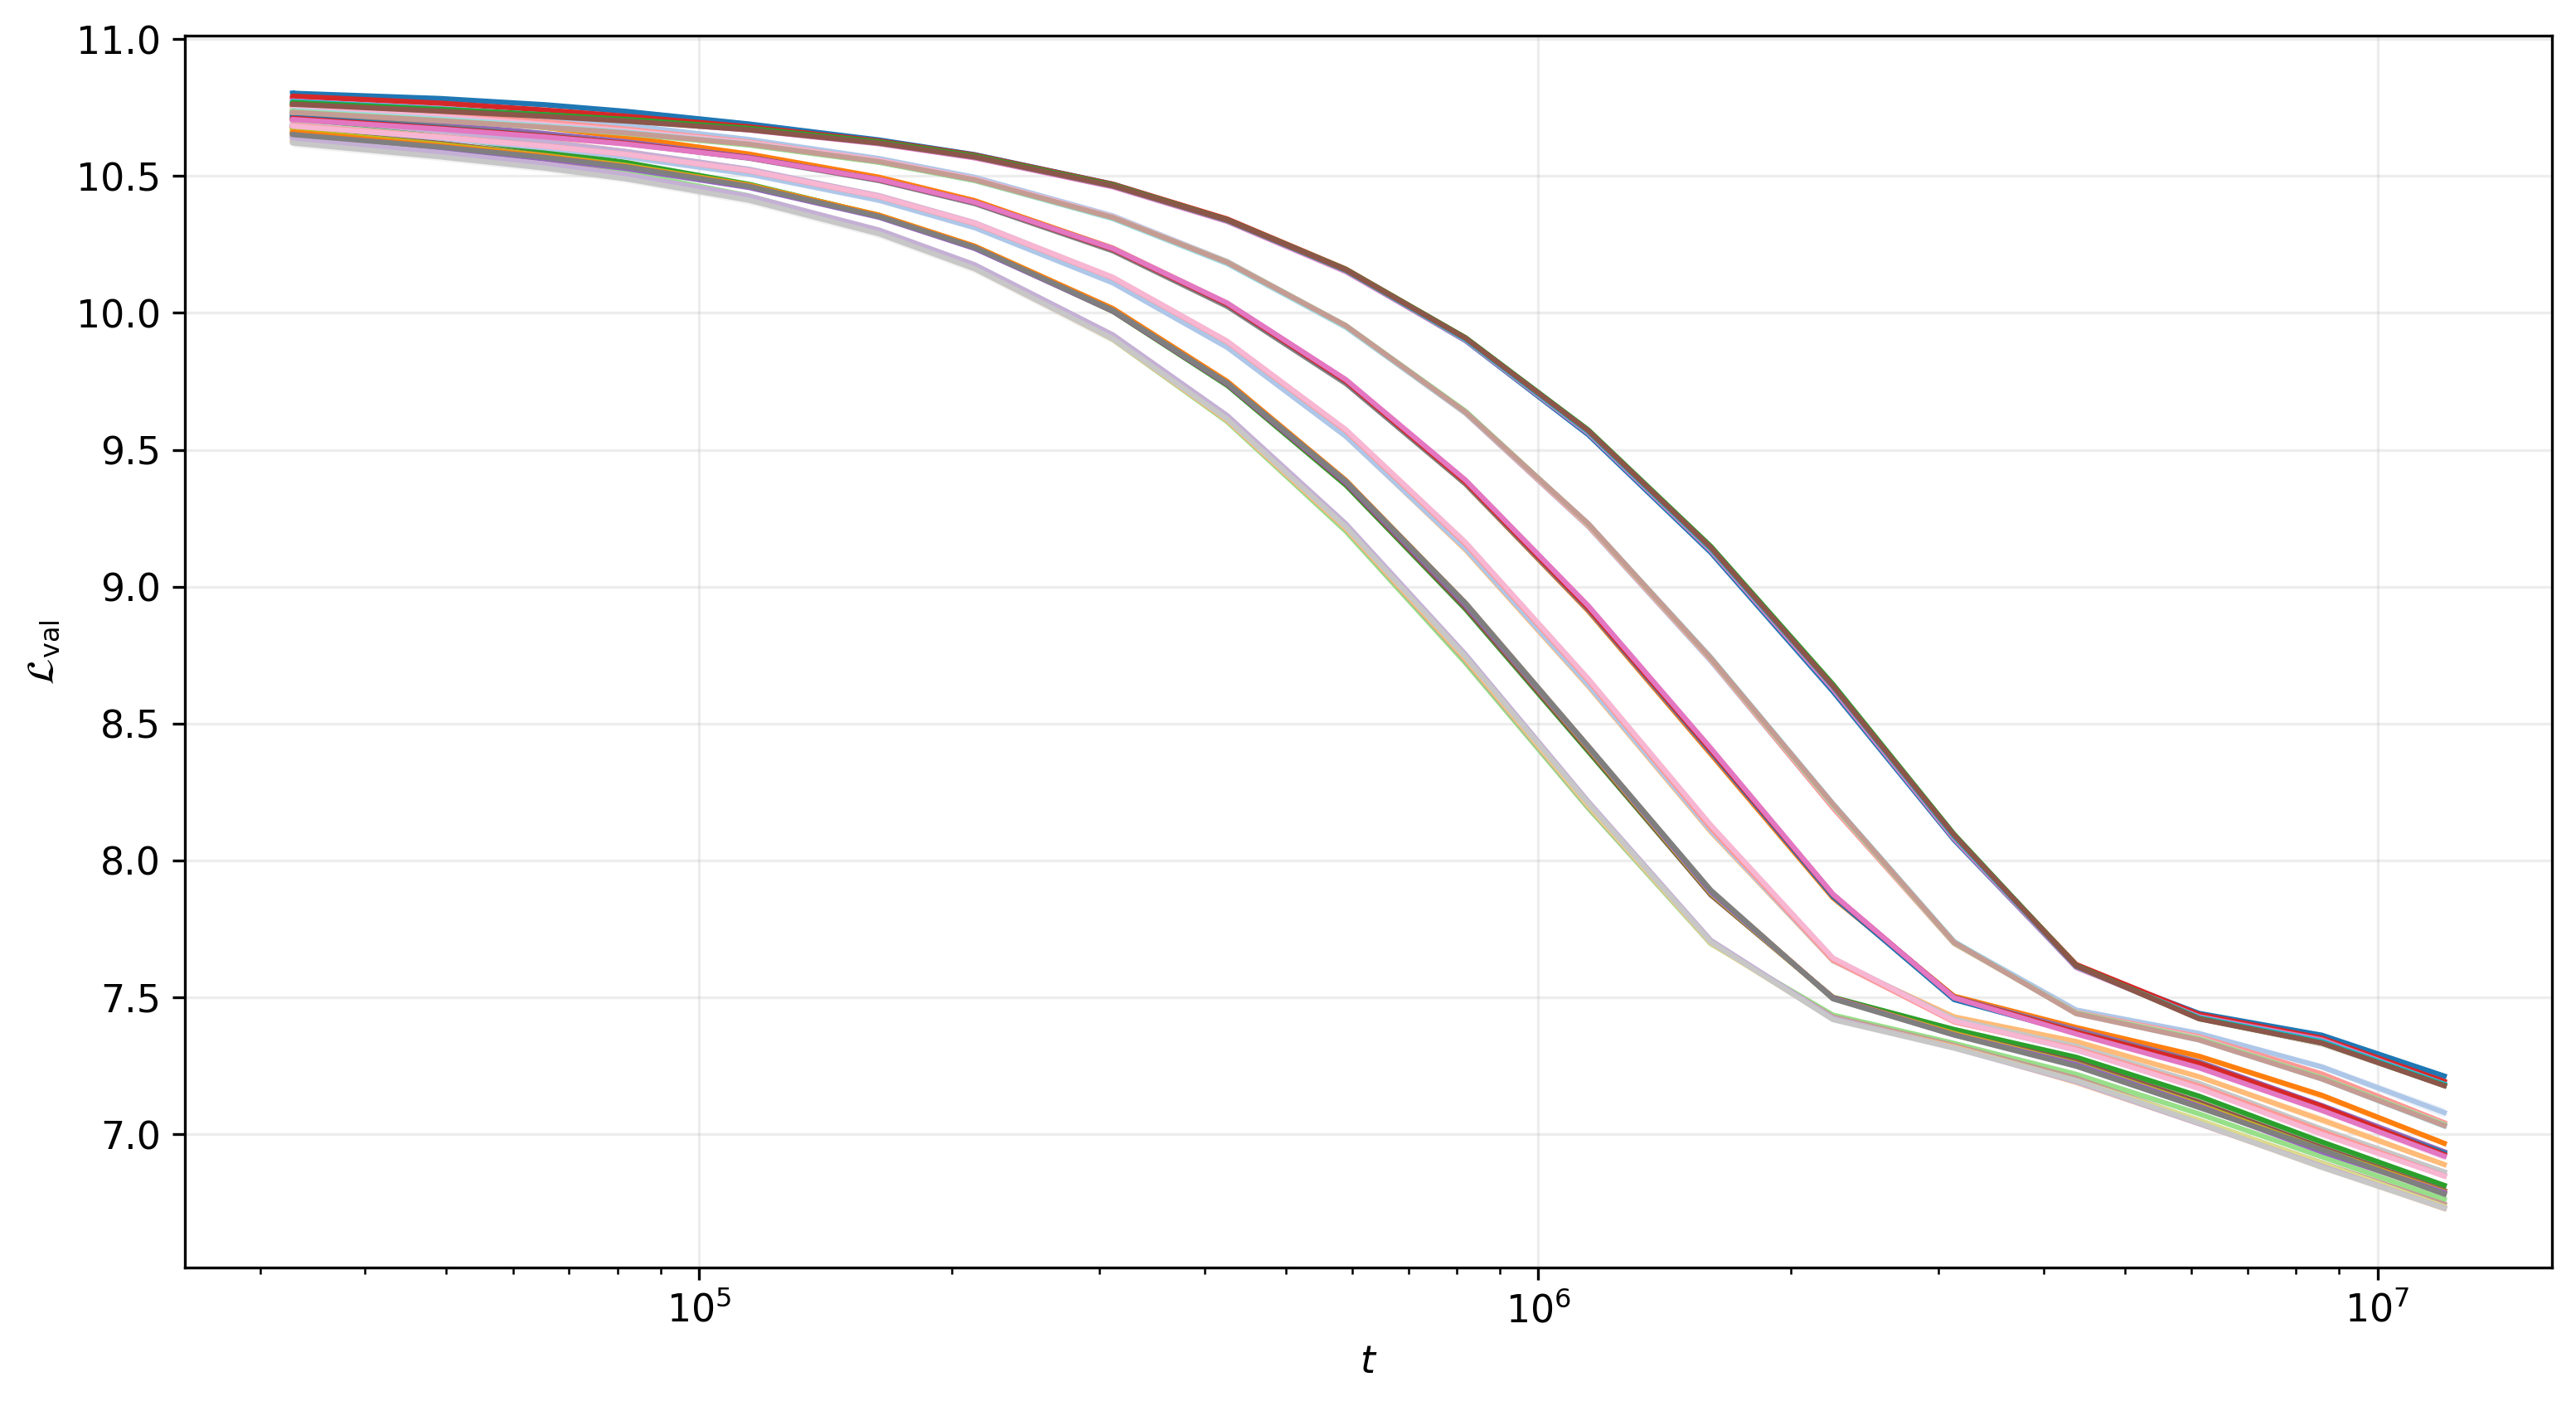
\includegraphics[width=\linewidth]{thesis/figures/chapter-1/empirical-landscape/fig_loss_all_models}\\[2pt]{\footnotesize валидационная ошибка}\end{minipage}\hfill
\begin{minipage}[t]{0.30\textwidth}\centering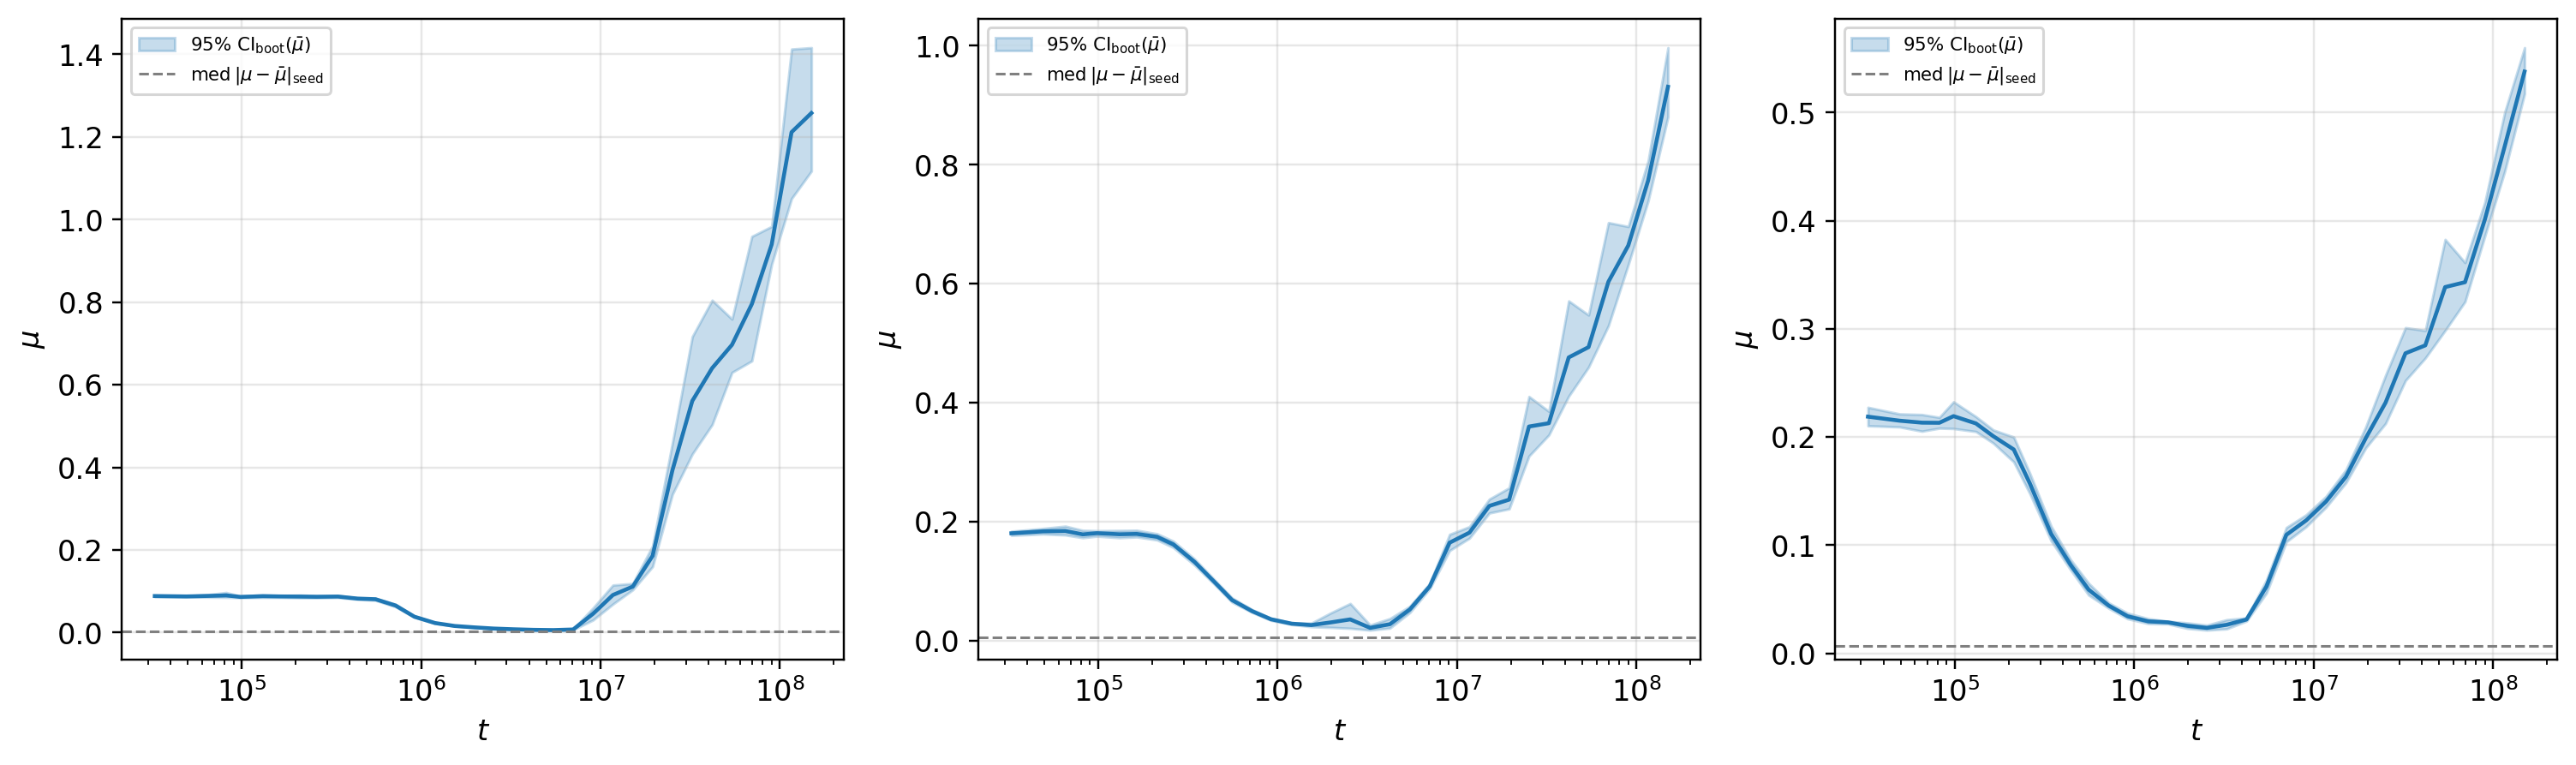
\includegraphics[width=\linewidth]{thesis/figures/chapter-1/empirical-landscape/fig_mu_seed_dispersion}\\[2pt]{\footnotesize среднее $\mu$ по $8$ запускам}\end{minipage}
\end{figure}
\smallskip
\begin{itemize}
    \setlength{\itemsep}{2pt}
    \item Оценка $\mu$ на каждой контрольной точке: новая мини-выборка $D_{\mathrm{probe}}$ из $m=8$ контекстов, $r=4$ независимых случайных направления (нижняя оценка спектральной нормы).
    \item Динамика $\mu$ содержит информацию о геометрическом режиме обучения, не сводимую к динамике валидационной функции потерь.
    \item Величина $\mu$ несет вариацию, которую не объясняют простые линейные формы по паре $(\mathcal{L}_{\mathrm{val}},\ln t)$.
\end{itemize}
\key{Ландшафтная мера дополняет валидационную функцию потерь как средство мониторинга обучения.}
\end{frame}

%----------------------------------------------------------------------------------------------------------
\section{Достаточный размер выборки}
%----------------------------------------------------------------------------------------------------------
\begin{frame}{Достаточный размер выборки}
\justifying
\footnotesize
\begin{rusdefinition}
    Размер выборки~$m^*$ называется достаточным согласно критерию~$T$, если~$T$ выполняется для всех~$k\ge m^*$.
\end{rusdefinition}
\begin{rusdefinition}
    При $\mu_D(D')=C\lvert D'\rvert$ условная сложность выборки выражается через достаточный размер: $m^*=\mu_D(D\mid f)/C$.
\end{rusdefinition}
\begin{ruscorollary}
    Ландшафтная мера связывается с приращением эмпирического риска. При $\|\boldsymbol{\theta}-\boldsymbol{\theta}^*\|_2\le R$
    \[
        \bigl|\mathcal{L}_{k+1}(\boldsymbol{\theta})-\mathcal{L}_k(\boldsymbol{\theta})\bigr|
        \le\frac{2M_\ell+\bar\mu_f\,R^2}{k+1}.
    \]
    Поэтому критерий $\bigl|\mathcal{L}_{k+1}-\mathcal{L}_k\bigr|\le\varepsilon$ выполняется при
    \[
        k+1\ge\frac{2M_\ell+\bar\mu_f\,R^2}{\varepsilon}.
    \]
    В среднем по выборке (при $\bar\mu_f\asymp\mu_f(f\mid D)$) величина $\bar\mu_f$ заменяется на ландшафтную меру $\mu_f(f\mid D)$.
\end{ruscorollary}
\key{Порядок достаточного размера выборки~$m^*$ определяется ландшафтной мерой модели.}
\end{frame}
%----------------------------------------------------------------------------------------------------------
\begin{frame}{Двусторонняя оценка достаточного размера выборки}
\justifying
\footnotesize
\begin{rustheorem}[Грабовой]
    Пусть заданы точка $\boldsymbol{\theta}^*$, число $R>0$ и выполнены условия.
    \begin{enumerate}[1)]
        \item $\ell(f_{\boldsymbol{\theta}}(\mathbf{x}_i),\mathbf{y}_i)$ имеет непрерывные третьи производные по $\boldsymbol{\theta}$ для всех $i$ и всех $\boldsymbol{\theta}\in B_R(\boldsymbol{\theta}^*)$.
        \item существуют константы $M_\ell,L_3\ge 0$: $\bigl|\ell(f_{\boldsymbol{\theta}^*}(\mathbf{x}_i),\mathbf{y}_i)\bigr|\le M_\ell$ и $\bigl\|\nabla^{3}_{\boldsymbol{\theta}}\ell(f_{\boldsymbol{\theta}}(\mathbf{x}_i),\mathbf{y}_i)\bigr\|_2\le L_3$ для всех $i$ и всех $\boldsymbol{\theta}\in B_R(\boldsymbol{\theta}^*)$.
        \item для некоторого $\varepsilon_g\ge 0$: $\bigl\|\nabla\mathcal{L}_k(\boldsymbol{\theta}^*)\bigr\|_2\le\varepsilon_g$ и $\bigl\|\nabla\mathcal{L}_{k+1}(\boldsymbol{\theta}^*)\bigr\|_2\le\varepsilon_g$.
        \item радиус $R$ меньше расстояния от $\boldsymbol{\theta}^*$ до границы области, в которой функции $\ell(f_{\boldsymbol{\theta}}(\mathbf{x}_i),\mathbf{y}_i)$ трижды непрерывно дифференцируемы (в частности, до границы линейной области кусочно-линейной сети).
    \end{enumerate}
    Обозначим $\bar\mu_f=\max_i\|\mathbf{H}_i(\boldsymbol{\theta}^*)-\bar{\mathbf{H}}\|_2$ и $A_1:=2M_\ell+\bar\mu_f R^2+L_3 R^3$. Тогда для любого $k\ge 1$
    \[
        \bigl|\mathcal{L}_{k+1}(\boldsymbol{\theta})-\mathcal{L}_k(\boldsymbol{\theta})\bigr|
        \le\frac{A_1}{k+1}+2\varepsilon_gR,
    \]
    и при $2\varepsilon_gR<\varepsilon$
    \[
        m^*\le\frac{A_1}{\varepsilon-2\varepsilon_gR}.
    \]
    Если дополнительно $\varepsilon_g=0$ и существуют единичный вектор $\mathbf{v}$, $\|\mathbf{v}\|_2=1$, и числа $c>0$, $\delta\in(0,1)$ такие, что с вероятностью не менее $1-\delta$ по случайному выбору $(k+1)$-го объекта выполнено $\bigl|\mathbf{v}^{\top}\bigl(\mathbf{H}_{k+1}(\boldsymbol{\theta}^*)-\mathbf{H}^{(k)}(\boldsymbol{\theta}^*)\bigr)\mathbf{v}\bigr|\ge c\,\bar\mu_f$ и $c\,\bar\mu_f>2L_3R$, то с вероятностью не менее $1-\delta$
    \[
        m^*\ge\frac{\tfrac12 R^2\bigl(c\,\bar\mu_f-2L_3R\bigr)-2M_\ell}{\varepsilon}-1 .
    \]
    При $2\varepsilon_gR\ll\varepsilon$, $c\,\bar\mu_f\asymp\bar\mu_f$, $\bar\mu_f R^2\gg M_\ell$ и $L_3R=O(\bar\mu_f)$ получаем $m^*=\Theta\bigl((M_\ell+\bar\mu_f R^2)/\varepsilon\bigr)$.
\end{rustheorem}
\key{Оценка двусторонняя: порядок $m^*$ определяется ландшафтной мерой, а не просто мажорируется ею.}
\end{frame}
%----------------------------------------------------------------------------------------------------------
\begin{frame}{Доказательство: двусторонняя оценка $m^*$}
\justifying
\footnotesize
\vspace{-2pt}
\textbf{Верхняя оценка.} Стабилизация $\bigl|\mathcal{L}_{k+1}-\mathcal{L}_k\bigr|\le\varepsilon$ при $\dfrac{A_1}{k+1}+2\varepsilon_gR\le\varepsilon$:
\[
    m^*\le m^*_{\mathrm{up}}:=\frac{A_1}{\varepsilon-2\varepsilon_gR},\qquad A_1=2M_\ell+\bar\mu_f R^2+L_3 R^3 .
\]
\textbf{Нижняя оценка.} По обратному неравенству треугольника, $\boldsymbol{\delta}=R\mathbf{v}$, $\|\mathbf{v}\|_2=1$:
\begin{align*}
    \bigl|\mathcal{L}_{k+1}-\mathcal{L}_k\bigr|
    &\ge\tfrac12 R^2\bigl|\mathbf{v}^{\top}\bigl(\mathbf{H}^{(k+1)}(\boldsymbol{\xi}_1)-\mathbf{H}^{(k)}(\boldsymbol{\xi}_2)\bigr)\mathbf{v}\bigr|-2M_\ell\\
    &\ge\tfrac12 R^2\bigl(c\,\bar\mu_f-2L_3R\bigr)-2M_\ell .
\end{align*}
Стабилизация невозможна при $k<m^*_{\mathrm{low}}:=\tfrac{1}{\varepsilon}\bigl(\tfrac12 R^2(c\,\bar\mu_f-2L_3R)-2M_\ell\bigr)-1$, откуда $m^*_{\mathrm{low}}\le m^*\le m^*_{\mathrm{up}}$.

\textbf{Ключевое.} Верхняя --- мажорирование по всем $k$, а нижняя требует $\bigl|\mathbf{v}^{\top}(\mathbf{H}_{k+1}-\mathbf{H}_k)\mathbf{v}\bigr|\ge c\,\bar\mu_f$ на нетривиальном множестве, поэтому «для всех $k$» ломается.
\vspace{-2pt}
\begin{center}
\begin{tikzpicture}[font=\footnotesize,>=stealth]
    \draw[->] (-3.4,0)--(3.4,0) node[right]{$m^*$};
    \draw[very thick,darkcyan] (-3.2,0)--(-0.7,0);
    \draw[very thick,darkgreen] (0.7,0)--(3.2,0);
    \node[below,darkcyan,align=center] at (-2.0,-0.32){$\le m^*_{\mathrm{up}}=\frac{A_1}{\varepsilon-2\varepsilon_gR}$};
    \node[below,darkgreen,align=center] at (2.0,-0.32){$\ge m^*_{\mathrm{low}}=\frac{K}{\varepsilon}-1$};
\end{tikzpicture}
\end{center}
\vspace{-6pt}
\key{При $\bar\mu_f R^2\gg M_\ell$, $L_3R=O(\bar\mu_f)$ получаем $m^*=\Theta\bigl((M_\ell+\mu_f(f\mid D)R^2)/\varepsilon\bigr)$.}
\end{frame}
%----------------------------------------------------------------------------------------------------------
\begin{frame}{Асимптотическая оценка $m^*$ через ландшафтную меру}
\justifying
\footnotesize
\begin{ruscorollary}
    Пусть выполнены условия теоремы о двусторонней оценке достаточного размера выборки и, дополнительно, $\bar\mu_f\asymp\mu_f(f\mid D)$, где
    \[
        \mu_f(f\mid D)=\mathbb{E}_{i}\bigl\|\mathbf{H}_i(\boldsymbol{\theta}^*)-\mathbb{E}_{j}\mathbf{H}_j(\boldsymbol{\theta}^*)\bigr\|_2
    \]
    --- ландшафтная мера сложности модели. Тогда при $2\varepsilon_gR\ll\varepsilon$, $\bar\mu_f R^2\gg M_\ell$ и $L_3R=O(\bar\mu_f)$
    \[
        m^*=\Theta\!\left(\frac{M_\ell+\mu_f(f\mid D)\,R^2}{\varepsilon}\right).
    \]
\end{ruscorollary}
\begin{rusremark}
    Ландшафтная мера есть среднее разброса пообъектных матриц Гессе $\mu_f(f\mid D)=\mathbb{E}_{i}\|\mathbf{H}_i(\boldsymbol{\theta}^*)-\bar{\mathbf{H}}\|_2$, а $\bar\mu_f=\max_{i}\|\mathbf{H}_i(\boldsymbol{\theta}^*)-\bar{\mathbf{H}}\|_2$, поэтому $\mu_f(f\mid D)\le\bar\mu_f$, и при $\bar\mu_f\asymp\mu_f(f\mid D)$ эти величины имеют одинаковый порядок.
\end{rusremark}
\begin{rusremark}
    Условия теоремы имеют разный статус. Верхняя граница опирается лишь на конечность $M_\ell$, $L_3$ и $\bar\mu_f$ и на ограничение стационарности $2\varepsilon_gR<\varepsilon$. Содержательным является условие нижней оценки о существовании направления $\mathbf{v}$ с ненулевым разбросом приростной кривизны.
\end{rusremark}
\key{Порядок достаточного размера выборки выражается прямо через ландшафтную меру сложности модели.}
\end{frame}
%----------------------------------------------------------------------------------------------------------
\begin{frame}{Стабилизация достаточного размера выборки на реальных данных}
\justifying
\small
\begin{center}
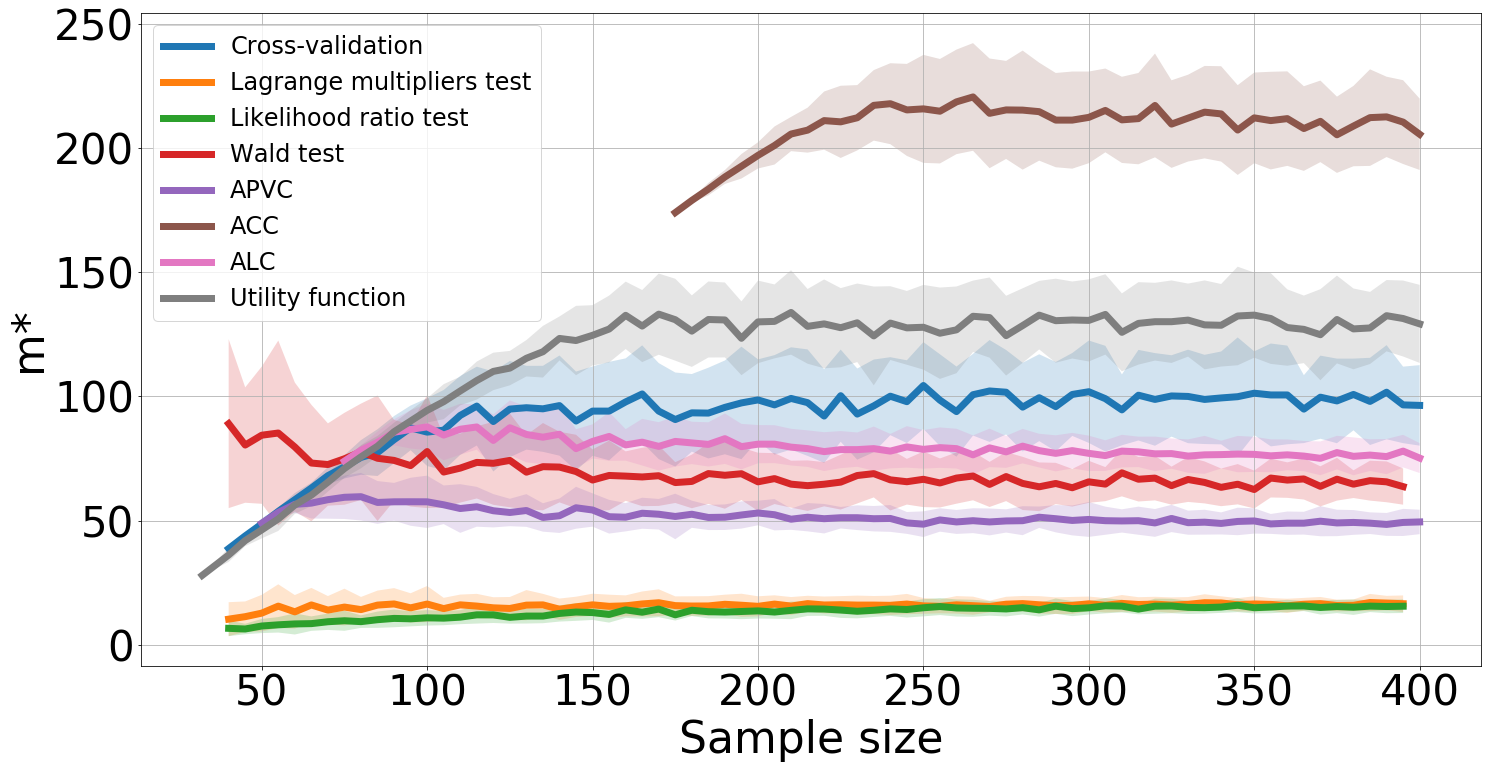
\includegraphics[width=0.46\textwidth]{thesis/figures/chapter-3/statical/graphs.png}\hfill
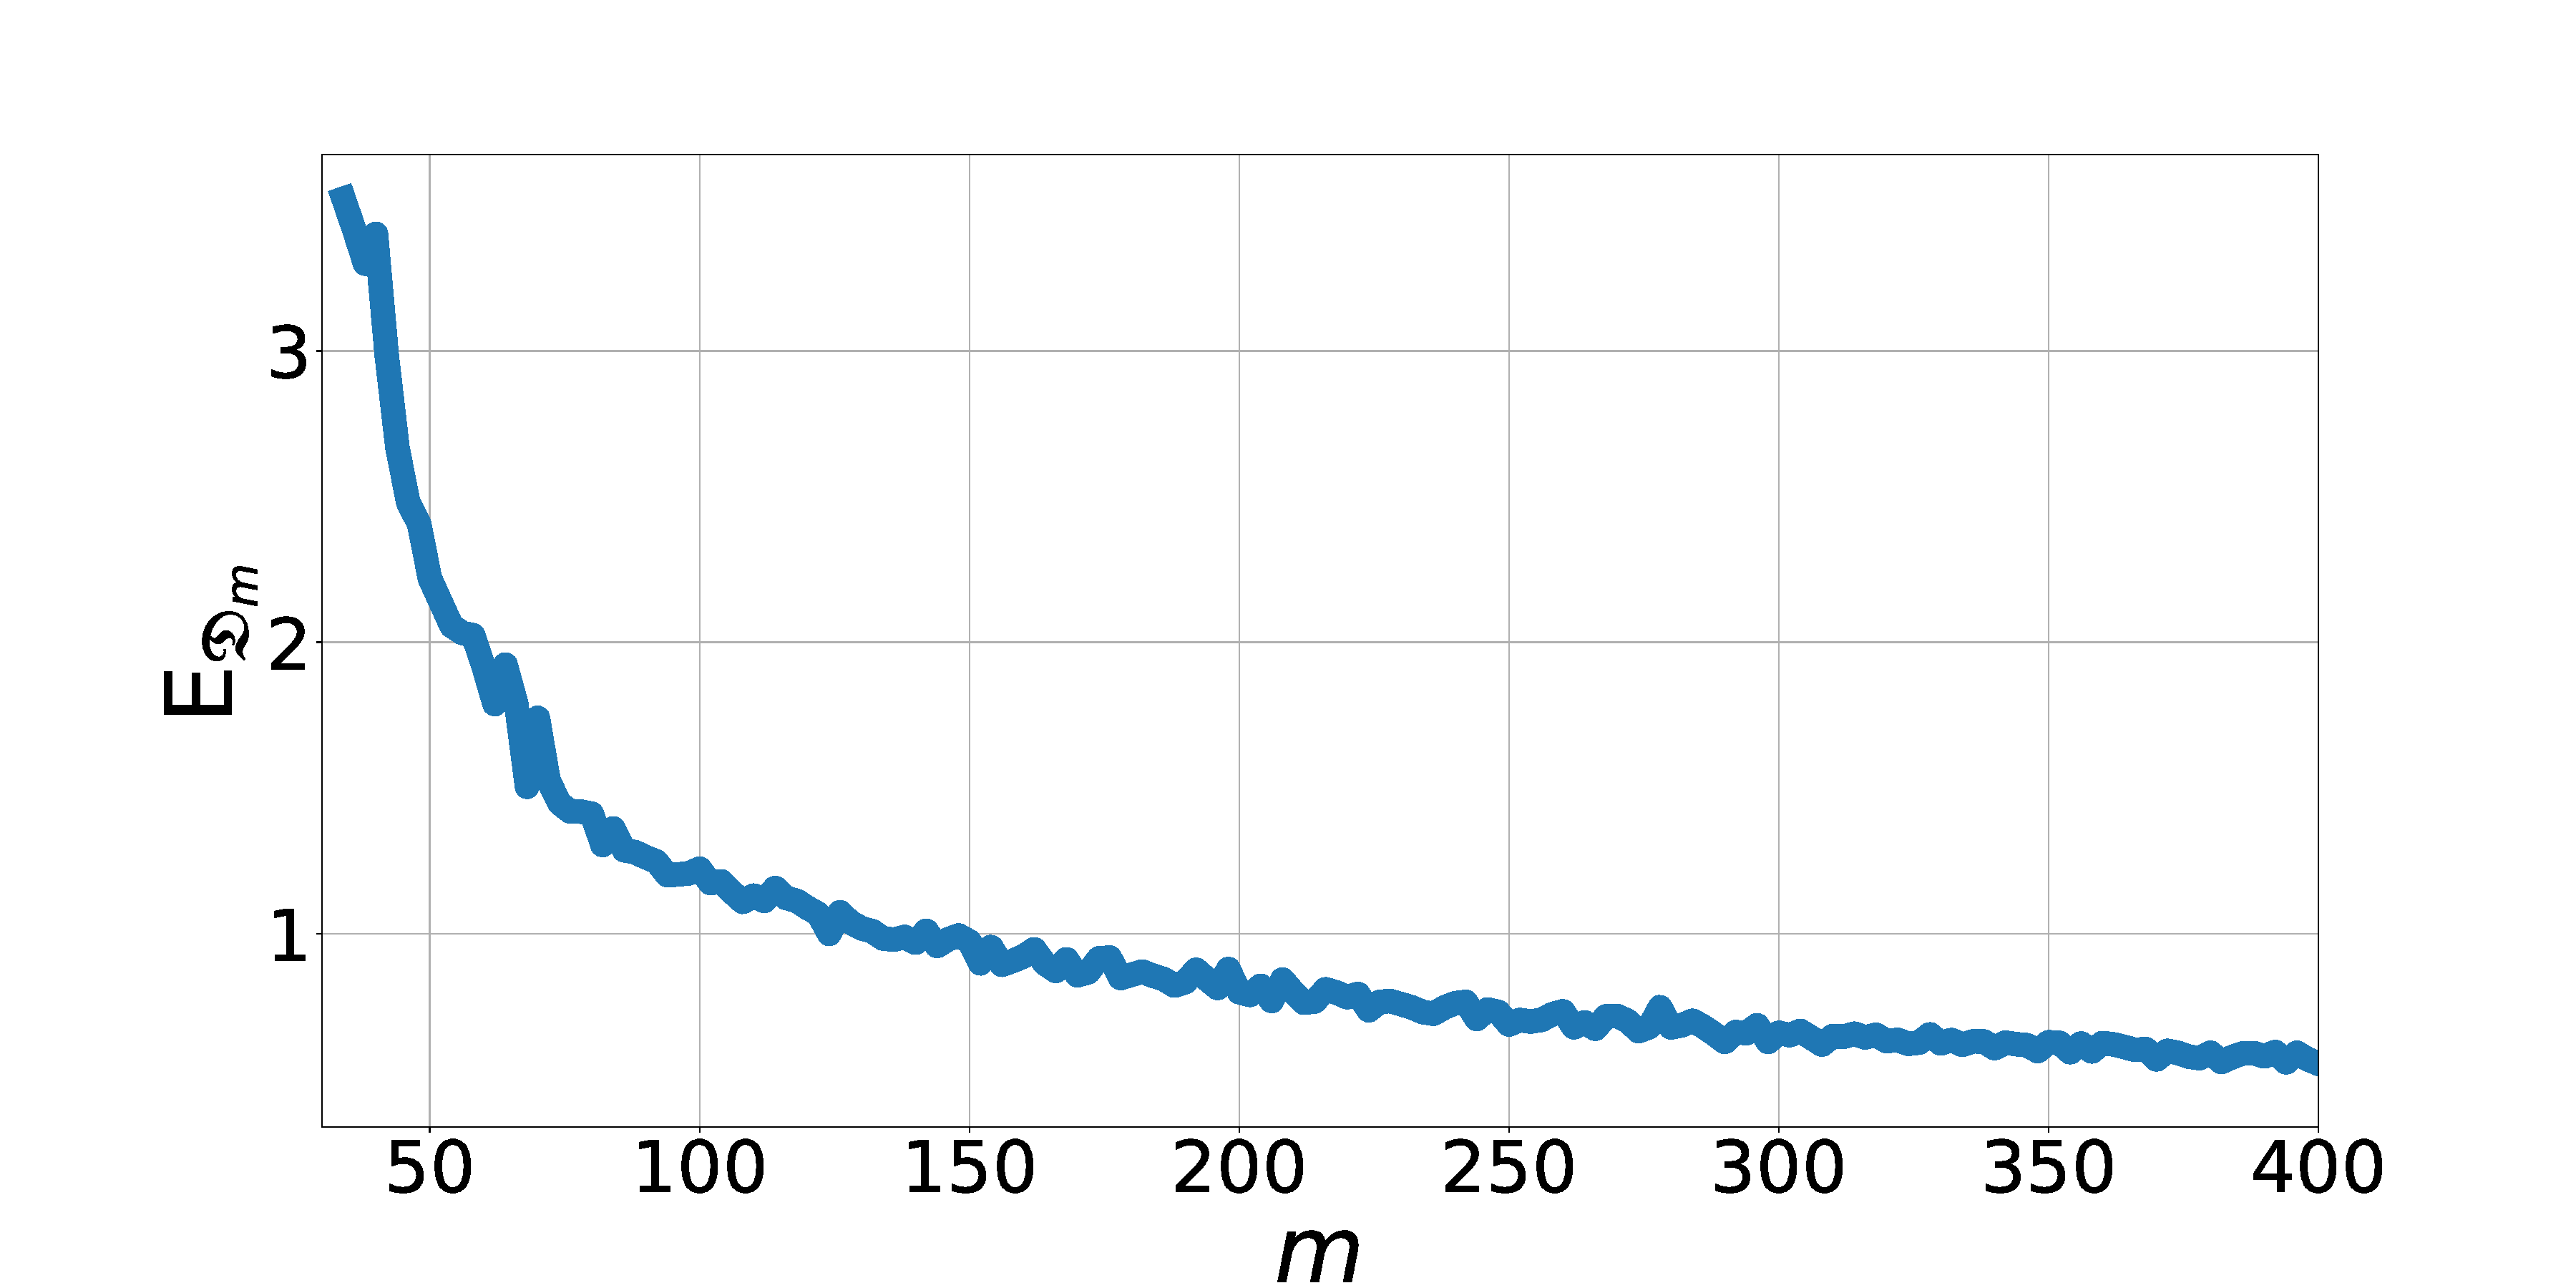
\includegraphics[width=0.46\textwidth]{thesis/figures/chapter-3/statical/bootstrap.pdf}
\end{center}
\vspace{2pt}
\begin{itemize}
    \setlength{\itemsep}{2pt}
    \item Оценки $m^*$ монотонны по размеру подвыборки и стремятся к константе (Boston Housing и др.).
    \item Низкая дисперсия оценок указывает на вычислительную устойчивость подхода.
    \item Стабилизация $m^*$ согласуется с асимптотическим порядком $m^*=\Theta\bigl((M_\ell+\mu_f(f\mid D)\,R^2)/\varepsilon\bigr)$.
\end{itemize}
\begin{rusremark}
    Рост объема данных сглаживает ландшафт потерь ($\mu_f(f\mid D)$ убывает), поэтому оценка $m^*$ перестает расти и выходит на константу.
\end{rusremark}
\key{Оценка достаточного размера выборки стабилизируется при росте объема данных.}
\end{frame}
%----------------------------------------------------------------------------------------------------------
\section{Снижение сложности моделей}
%----------------------------------------------------------------------------------------------------------
\begin{frame}{Байесовская дистилляция: сохранение нормальности}
\justifying
\footnotesize
\begin{rusdefinition}
    При совпадении архитектур априорное распределение ученика задается апостериорным распределением учителя~$p(\mathbf{u}|\mathfrak{D})=\mathcal{N}(\mathbf{m},\boldsymbol{\Sigma})$.
\end{rusdefinition}
\begin{rustheorem}[Грабовой]
    Пусть выполняются условия: (1) $p(\mathbf{u}|\mathfrak{D})=\mathcal{N}(\mathbf{m},\boldsymbol{\Sigma})$, (2) $T=L$, (3) $n_t^{(\mathrm{tr})}\ge n_t^{(\mathrm{st})}$. Пусть преобразование $\boldsymbol{\phi}(t,\mathbf{u})$ удаляет один нейрон из $t$-го слоя модели учителя, а $\boldsymbol{\upsilon}=\boldsymbol{\phi}(t,\mathbf{u})$ --- вектор оставшихся параметров. Тогда распределение параметров после такого преобразования также является нормальным: $p(\boldsymbol{\upsilon}|\mathfrak{D})=\mathcal{N}(\boldsymbol{\mu}_{\boldsymbol{\upsilon}},\boldsymbol{\Xi}_{\boldsymbol{\upsilon},\boldsymbol{\upsilon}})$.
\end{rustheorem}
Параметры условного нормального распределения (полный вектор и подвектор, соответствующий~$\boldsymbol{\upsilon}$):
\[
    \boldsymbol{\mu}=\mathbf{m}_{\bar{\nu}_1}+\boldsymbol{\Sigma}_{\bar{\nu}_1,\nu_1}\boldsymbol{\Sigma}_{\nu_1,\nu_1}^{-1}\bigl(\mathbf{0}-\mathbf{m}_{\nu_1}\bigr),\qquad
    \boldsymbol{\Xi}=\boldsymbol{\Sigma}_{\bar{\nu}_1,\bar{\nu}_1}-\boldsymbol{\Sigma}_{\bar{\nu}_1,\nu_1}\boldsymbol{\Sigma}_{\nu_1,\nu_1}^{-1}\boldsymbol{\Sigma}_{\nu_1,\bar{\nu}_1},
\]
\[
    \boldsymbol{\mu}_{\boldsymbol{\upsilon}}=[\boldsymbol{\mu}]_{\boldsymbol{\upsilon}},\qquad
    \boldsymbol{\Xi}_{\boldsymbol{\upsilon},\boldsymbol{\upsilon}}=[\boldsymbol{\Xi}]_{\boldsymbol{\upsilon},\boldsymbol{\upsilon}},
\]
где $\bar{\nu}_1=\bigl[\boldsymbol{\upsilon}^{\top},\nu_2^{\top}\bigr]^{\top}$, $\nu_1$ --- удаляемый нейрон.
\begin{rustheorem}[Грабовой]
    Пусть выполняются условия: (1) $p(\mathbf{u}|\mathfrak{D})=\mathcal{N}(\mathbf{m},\boldsymbol{\Sigma})$, (2) $n_t^{(\mathrm{tr})}=n_{t-1}^{(\mathrm{tr})}$ (матрица $\mathbf{U}_t$ квадратная), (3) $\boldsymbol{\sigma}\circ\boldsymbol{\sigma}=\boldsymbol{\sigma}$. Пусть $\boldsymbol{\psi}(t,\mathbf{u})$ удаляет $t$-й слой модели учителя, а $\boldsymbol{\upsilon}=\boldsymbol{\psi}(t,\mathbf{u})$ --- вектор оставшихся параметров. Тогда апостериорное распределение оставшихся параметров также является нормальным.
\end{rustheorem}
\key{Сохранение нормальности выравнивает пространства параметров учителя и ученика при различающихся архитектурах.}
\end{frame}
%----------------------------------------------------------------------------------------------------------
\begin{frame}[t]{Многодоменная дистилляция}
\justifying
\small
\begin{rusdefinition}
    Генеральная совокупность объектов~$B$ называется близкой к генеральной совокупности~$A$, если существует инъективное отображение~$\varphi:\mathbb{X}_{\mathrm{t}}\to\mathbb{X}_{\mathrm{s}}$, связывающее целевую (малоресурсную) выборку с исходной выборкой учителя, и сдвиг доменов мал: $s:=\max_i\|\varphi(\mathbf{x}_i)-\mathbf{x}_i\|_2$ ограничен. Содержательность условия определяется малостью $s$.
\end{rusdefinition}
Функция потерь, учитывающая метки учителя и связь между доменами:
\[
    \resizebox{0.98\textwidth}{!}{$\textstyle\mathcal{L}(\mathbf{w},\mathbf{X},\mathbf{Y},f,\varphi)=-\lambda\sum_{i=1}^{m}\sum_{r=1}^{R}\mathbb{I}[y_i=r]\log g^{r}(\mathbf{x}_i,\mathbf{w})-(1-\lambda)\sum_{i=1}^{m}\sum_{r=1}^{R}(f\circ\varphi)^{r}(\mathbf{x}_i)\log g^{r}(\mathbf{x}_i,\mathbf{w}).$}
\]
где $\lambda$ --- метапараметр, задающий вес дистилляции, $\mathbb{I}$ --- индикаторная функция.
\begin{rustheorem}
    Пусть $\varphi:\mathbb{X}_{\mathrm{t}}\to\mathbb{X}_{\mathrm{s}}$ инъективно, $\mathbf{f}$ --- модель учителя, и выполнено: (1) существует единая точка $\boldsymbol{\theta}^*$ для $\mathbf{f}$ и $\mathbf{f}\circ\varphi$, (2) $\|\mathbf{H}^{\mathbf{f}}(\mathbf{x})-\mathbf{H}^{\mathbf{f}}(\mathbf{x}')\|_2\le L_H\|\mathbf{x}-\mathbf{x}'\|_2$, где $\mathbf{H}^{\mathbf{f}}(\mathbf{x}):=\nabla^2_{\boldsymbol{\theta}}\ell\bigl(\mathbf{f}_{\boldsymbol{\theta}}(\mathbf{x}),y\bigr)$. Тогда
    \[
        \mu_f(\mathbf{f}\circ\varphi\mid\mathfrak{D}_{\mathrm{t}})=\mu_f\bigl(\mathbf{f}\mid\varphi(\mathfrak{D}_{\mathrm{t}})\bigr),\qquad
        \mu_f\bigl(\mathbf{f}\mid\varphi(\mathfrak{D}_{\mathrm{t}})\bigr)\le\mu_f\bigl(\mathbf{f}\mid\mathfrak{D}_{\mathrm{t}}\bigr)+2L_H s,
    \]
    где $s:=\max_i\|\varphi(\mathbf{x}_i)-\mathbf{x}_i\|_2$. Неувеличение меры гарантируется при $\mu_f(\mathbf{f}\mid\mathfrak{D}_{\mathrm{t}})+2L_Hs\le\mu_f(\mathbf{f}\mid\mathfrak{D}_{\mathrm{s}})$.
\end{rustheorem}
\key{Инъективное~$\varphi$ не увеличивает меру учителя сверх~$\mu_f(\mathbf{f}\mid\mathfrak{D}_{\mathrm{t}})+2L_H s$ при ограниченном сдвиге доменов.}
\end{frame}
%----------------------------------------------------------------------------------------------------------
\begin{frame}{Доказательство: отображение $\varphi$ не увеличивает меру}
\justifying
\footnotesize
\vspace{-2pt}
Цель: $\mu_f(\mathbf{f}\circ\varphi\mid\mathfrak{D}_{\mathrm{t}})\le\mu_f(\mathbf{f}\mid\mathfrak{D}_{\mathrm{t}})+2L_H s$. Опора --- цепное правило и липшицевость гессиана.
\begin{enumerate}[1)]
    \item \textbf{Цепное правило.} $\nabla^2_{\boldsymbol{\theta}}\bigl[\ell(\mathbf{f}_{\boldsymbol{\theta}}(\varphi(\mathbf{x})),y)\bigr]=\mathbf{H}^{\mathbf{f}}(\varphi(\mathbf{x}))$.
    \item \textbf{Равенство мер.} $\mu_f(\mathbf{f}\circ\varphi\mid\mathfrak{D}_{\mathrm{t}})=\mu_f\bigl(\mathbf{f}\mid\varphi(\mathfrak{D}_{\mathrm{t}})\bigr)$.
    \item \textbf{Липшицевость.} $\bigl\|\mathbf{H}^{\mathbf{f}}(\mathbf{x})-\mathbf{H}^{\mathbf{f}}(\mathbf{x}')\bigr\|_2\le L_H\|\mathbf{x}-\mathbf{x}'\|_2$ и неравенство треугольника:
    \[
        \bigl\|\mathbf{H}_i-\bar{\mathbf{H}}\bigr\|_2\le\bigl\|\mathbf{H}_i^{0}-\bar{\mathbf{H}}^{0}\bigr\|_2+2L_H s,\quad s=\max_i\|\varphi(\mathbf{x}_i)-\mathbf{x}_i\|_2.
    \]
\end{enumerate}
Усредняя по $i$: $\mu_f\bigl(\mathbf{f}\mid\varphi(\mathfrak{D}_{\mathrm{t}})\bigr)\le\mu_f\bigl(\mathbf{f}\mid\mathfrak{D}_{\mathrm{t}}\bigr)+2L_H s$.
\vspace{-2pt}
\key{Гессиан композиции = гессиан учителя в $\varphi(\mathbf{x})$; сдвиг доменов входит с коэффициентом $2L_H s$.}
\end{frame}
%----------------------------------------------------------------------------------------------------------
\begin{frame}{Прореживание по ковариации градиентов}
\justifying
\footnotesize
Порядок на множестве параметров модели задается при помощи ковариационной матрицы~$\mathbf{C}$ градиентов функции ошибки~$\mathcal{L}$ по параметрам~$\mathbf{w}$.
\[
    \mathbf{C}_t=(1-\kappa_t)\mathbf{C}_{t-1}+\kappa_t\bigl(\mathbf{g}_{1,t}-\mathbf{g}_{S,t}\bigr)\bigl(\mathbf{g}_{1,t}-\mathbf{g}_{S,t}\bigr)^{\mathsf{T}},
\]
где $\mathbf{g}_{S,t}$ --- значение градиента на подвыборке размера~$S$, $\mathbf{g}_{1,t}$ --- на первом ее элементе, $\kappa_t=1/t$. Матрица $\mathbf{C}_t$ задает оценку ковариации градиентов (по вкладу первого элемента подвыборки относительно общего градиента) и используется для задания порядка на параметрах.

Введем $\mathbf{J}_i=\nabla_{\boldsymbol{\theta}}z_i$, $g_i=\partial\ell_i/\partial z$, $A_i=\partial^2\ell_i/\partial z^2$ и обозначим
\[
    \mathbf{C}=\mathbb{E}[\nabla\ell\,\nabla\ell^{\top}],\quad
    \mathbf{H}_O=\mathbb{E}[A_i\mathbf{J}_i\mathbf{J}_i^{\top}],\quad
    \mathbf{H}=\mathbb{E}[\nabla^2\ell_i],\quad
    \mathbf{R}=\mathbb{E}[g_i\nabla^2z_i].
\]
\begin{rusproposition}[Грабовой]
    Пусть выполнено $\mathbb{E}\bigl[g_i^2\mid\mathbf{J}_i,\mathbf{x}_i\bigr]=A_i$, где математическое ожидание берется по модельной вероятности $p_\theta(y\mid x)$, а не по эмпирическому распределению данных, $\ell_i\in C^2$, $\|\nabla^2z_i\|_2\le M_2$, $\|\mathbf{J}_i\|_2\le M_{\mathbf{J}}$, $\mathbb{E}\lvert g_i\rvert\le m_g$. Тогда
    \[
        \mathbf{C}=\mathbf{H}_O,\qquad \mathbf{H}=\mathbf{H}_O+\mathbf{R}=\mathbf{C}+\mathbf{R},\qquad \|\mathbf{R}\|_2\le M_2\,m_g.
    \]
\end{rusproposition}
Иллюстрация тождества $\mathbf{C}=\mathbf{H}_O$: GN-компонента есть фишеровская информация $\mathbf{H}_O=\mathbb{E}\bigl[\nabla\log p_\theta\,\nabla\log p_\theta^{\top}\bigr]$, а градиент потерь $g_i=-\nabla\log p_\theta(y_i\mid x_i)$, поэтому при $y_i\sim p_\theta(\cdot\mid x_i)$ (модельная вероятность из условия) $\mathbb{E}\bigl[g_i g_i^{\top}\mid x_i\bigr]=\mathbf{H}_O(x_i)$. Следовательно, прореживание по $\mathbf{C}$ режет именно ландшафтно-значимую GN-компоненту $\mathbf{H}_O$, а не нерелевантную $\mathbf{R}$ в декомпозиции $\mathbf{H}=\mathbf{H}_O+\mathbf{R}$.
Процедура прореживания. Обозначим~$\mathcal{I}_{\mathbf{w}_{t_0}}$ вектор индексов, порядок которого задан при помощи ковариационной матрицы~$\mathbf{C}_{t_0}$.
\[
    \alpha_i(\zeta)=\begin{cases}
        1,&\text{если }\mathcal{I}_{\mathbf{w}_{t_0}}[i]\le\zeta,\\
        0,&\text{иначе},
    \end{cases}\qquad
    \mathbf{w}_t=\mathbf{w}_{t-1}+\bm{\alpha}(\zeta)\cdot\Delta\mathbf{w}\bigl(\mathbf{g}_{S,t},\mathbf{w}_{t-1},\mathbf{w}_{t-2},\ldots\bigr),
\]
где $\zeta$ --- число обучаемых параметров. После умножения на бинарный вектор~$\bm{\alpha}$ координаты с~$\mathcal{I}_{\mathbf{w}_{t_0}}[i]\le\zeta$ обновляются, а остальные фиксируются.
\key{Ковариация градиентов совпадает с гаусс-ньютоновской компонентой Гессе.}
\end{frame}
%----------------------------------------------------------------------------------------------------------
\begin{frame}{Антидистилляция}
\justifying
\small
\setlength{\abovedisplayskip}{2pt}\setlength{\belowdisplayskip}{2pt}\setlength{\abovedisplayshortskip}{1pt}\setlength{\belowdisplayshortskip}{1pt}
Даны два набора данных $\mathfrak{D}_1$, $\mathfrak{D}_2$, модель учителя $\mathbf{g}_{\mathrm{tr}}$ обучена на~$\mathfrak{D}_1$, требуется построить более сложную модель ученика~$\mathbf{f}_{\mathrm{st}}$ на~$\mathfrak{D}_2$ ($N_{\mathrm{tr}}<N_{\mathrm{st}}$).
Отображение параметров учителя в начальные параметры ученика:
\[
    \boldsymbol{\varphi}:\mathbb{R}^{N_{\mathrm{tr}}}\to\mathbb{R}^{N_{\mathrm{st}}},\qquad \mathbf{w}=\boldsymbol{\varphi}(\hat{\mathbf{u}}).
\]
Расширение размерности решается минимизацией составной функции потерь:
\[
    \mathcal{L}(\mathbf{w})=\lambda_1\mathcal{L}_{\mathrm{ce}}(\mathbf{w},\mathfrak{D}_1)+\lambda_2\|\mathbf{u}-\mathrm{Pr}[\mathbf{w}]\|_2^2+\lambda_3\mathcal{L}_3^{\delta}(\mathbf{w},\mathfrak{D}_1)+\lambda_4\,\operatorname{tr}\!\Bigl(\tfrac{\partial^2\mathcal{L}_{\mathrm{ce}}}{\partial\mathbf{w}^2}\Bigr),
\]
\begin{align*}
    \mathcal{L}_{\mathrm{ce}}&=\text{перекрестная энтропия}, &\mathrm{Pr}&=\text{проекция общих параметров},\\
    \mathcal{L}_3^{\delta}&=\text{устойчивость к шуму во входах}, &\lambda_4\operatorname{tr}\!\Bigl(\tfrac{\partial^2\mathcal{L}_{\mathrm{ce}}}{\partial\mathbf{w}^2}\Bigr)&=\text{регуляризация следа Гессе},
\end{align*}
где $\lambda_i\ge 0$.
\begin{rusremark}
    \footnotesize
    Устойчивость к искажению входных данных обеспечивают слагаемое $\mathcal{L}_3^{\delta}$ и регуляризация следа Гессе: оба регулируют матрицу Гессе функции перекрестной энтропии, способствуя нахождению решений в более плоских областях ландшафта функции потерь.
\end{rusremark}
\begin{center}
\begin{scriptsize}
\begin{tabular}{|l|c|c|c|}
\hline
\textbf{Инициализация} & \textbf{Точность} & \textbf{FGSM} & \textbf{Шум} \\
\hline
Xavier & $0.68\pm0.08$ & $0.42\pm0.04$ & $0.58\pm0.06$ \\
Zero Pad & $\mathbf{0.86\pm0.02}$ & $0.50\pm0.01$ & $\mathbf{0.71\pm0.03}$ \\
Антидистилляция & $\mathbf{0.86\pm0.05}$ & $\mathbf{0.57\pm0.03}$ & $0.67\pm0.03$ \\
\hline
\end{tabular}
\end{scriptsize}
\end{center}
\key{Антидистилляция через регуляризацию следа Гессе повышает устойчивость к возмущениям.}
\end{frame}
%----------------------------------------------------------------------------------------------------------
\begin{frame}{LoRA-адаптеры: состоятельность оценки}
\justifying
\footnotesize
LoRA ограничивает $\Delta W$ условием низкого ранга путем факторизации:
\[
    \Delta W = A B, \quad A \in \mathbb{R}^{d \times r}, \ B \in \mathbb{R}^{r \times k}, \ r \ll \min(d,k),
\]
что сокращает число обучаемых параметров с $dk$ до $r(d+k)$.
\begin{rustheorem}[Грабовой]
    Пусть $\mathcal{D} = \{(X_i, c_i)\}_{i=1}^n$ --- независимые одинаково распределенные пары из распределения $P_{\mathrm{true}}$ на $\mathcal{X}\times[N_c]$, где $[N_c]=\{1,\ldots,N_c\}$. Рассмотрим компактное множество $K\subset\mathbb{R}^p$ и параметрическую модель $P_{\Phi_0+\Theta}(c\mid X)$ при $\Theta\in K$, где $\Phi_0$ --- замороженный вектор предобученных параметров. Предположим:
    \begin{enumerate}
        \item Существует единственная точка $\Theta^\star\in K$, минимизирующая ожидаемый риск $L(\Theta)=\mathbb{E}_{(X,c)\sim P_{\mathrm{true}}}[-\log P_{\Phi_0+\Theta}(c\mid X)]$, $\Theta\in K$.
        \item Функция $(X,c,\Theta)\mapsto-\log P_{\Phi_0+\Theta}(c\mid X)$ непрерывна на своей области допустимых значений и $\mathbb{E}_{(X,c)\sim P_{\mathrm{true}}}\bigl[\sup_{\Theta\in K}|\log P_{\Phi_0+\Theta}(c\mid X)|\bigr]<\infty$.
        \item Эмпирический риск задается в виде $\mathscr{L}_n(\Theta)=-\frac{1}{n}\sum_{i=1}^{n}\log P_{\Phi_0+\Theta}(c_i\mid X_i)$, а оценка $\widehat{\Theta}_n$ выбирается как измеримый минимизатор $\mathscr{L}_n$ на $K$ (если минимум достигается. Иначе --- $\varepsilon_n$-минимизатор с $\varepsilon_n\downarrow0$).
    \end{enumerate}
    Тогда $\widehat{\Theta}_n \xrightarrow{P} \Theta^\star$ при $n\to\infty$.
\end{rustheorem}
\begin{rusremark}
    Здесь $\Theta$ --- матрица обновления $\Delta W$, а не пара $(A,B)$: в силу $\Delta W=AB=(AC)(C^{-1}B)$ минимум по $(A,B)$ не единствен. Состоятельность понимается для произведения $AB$. Проверяемыми условиями состоятельности M-оценки в теореме являются: компактность $K$, единственность точки $\Theta^\star$ на $K$, непрерывность и интегрируемость $\sup_{\Theta\in K}|\log P_{\Phi_0+\Theta}|$, а также измеримость $\widehat{\Theta}_n$ как минимизатора эмпирического риска на $K$.
\end{rusremark}
\key{При низкоранговой параметризации оценка остается статистически состоятельной.}
\end{frame}
%----------------------------------------------------------------------------------------------------------
\begin{frame}{Число параметров и качество при LoRA}
\justifying
\small
\begin{minipage}[c]{0.48\textwidth}
    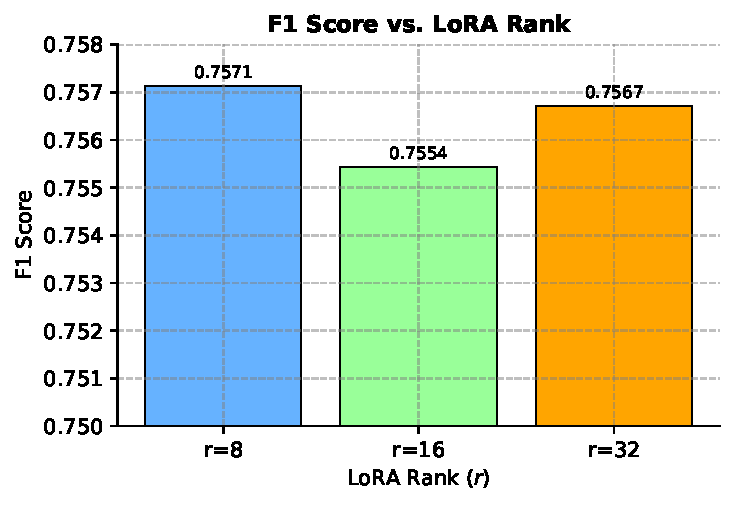
\includegraphics[width=\linewidth,height=0.36\textheight,keepaspectratio]{thesis/figures/chapter-5/rademacher/lora_rank_vs_f1-1.pdf}
\end{minipage}\hfill
\begin{minipage}[c]{0.47\textwidth}
\begin{scriptsize}
\begin{tabular}{lccc}
\hline
\textbf{Метрика} & \textbf{DeBERTa} & \textbf{LoRA} & \textbf{Изм.} \\
\hline
Точность $\uparrow$ & $0.7104$ & $0.6876$ & $-3.2\%$ \\
Полнота $\uparrow$ & $0.9608$ & $0.9470$ & $-1.4\%$ \\
$F_1$-мера $\uparrow$ & $0.7806$ & $0.7648$ & $-2.0\%$ \\
\hline
Потери $\downarrow$ & $1.8094$ & $\mathbf{1.1522}$ & $-36.3\%$ \\
Время, с $\downarrow$ & $5570$ & $\mathbf{4867}$ & $-12.6\%$ \\
\hline
\end{tabular}
\end{scriptsize}
\smallskip
\[\Delta W=AB,\quad r(d+k)\ll dk.\]
\end{minipage}

{\footnotesize Задача --- детекция машинно-генерированного текста.}
\smallskip
\begin{itemize}
    \setlength{\itemsep}{2pt}
    \item Исходные параметры замораживаются, низкоранговые адаптеры вставляются в каждый блок трансформера.
    \item Ранг~$r=8$, коэффициент масштабирования~$\alpha=32$, доля отсева~$0.1$.
    \item Обучаемыми остаются $296\,450$ параметров из $184$~млн общих~($\approx0.16\%$).
    \item Это согласуется с теоретической мотивацией снижения размерности.
\end{itemize}
\begin{rusremark}
    При ранге~$r=8$ и $\alpha=32$ пороговые метрики качества снижаются на $1{,}4$--$3{,}2\%$, тогда как потери на валидации и время обучения сокращаются на $36{,}3\%$ и $12{,}6\%$. Различие объясняется тем, что потери и пороговые метрики --- разные функционалы: LoRA дает более гладкую динамику обучения и меньшие потери, при этом $F_1$ падает на $2{,}0\%$ в пределах того же диапазона.
\end{rusremark}
\key{LoRA снижает число обучаемых параметров при малом изменении качества.}
\end{frame}
%----------------------------------------------------------------------------------------------------------
\begin{frame}{Радемахеровская сложность многозадачного обучения}
\justifying
\scriptsize
\setlength{\abovedisplayskip}{2pt}\setlength{\belowdisplayskip}{2pt}\setlength{\abovedisplayshortskip}{1pt}\setlength{\belowdisplayshortskip}{1pt}
\setlength{\parskip}{0.5pt}
\setlength{\itemsep}{1pt}\setlength{\parsep}{0pt}\setlength{\parindent}{0pt}
\begin{rustheorem}[Грабовой]
    Пусть $S_t=\{x_i\}_{i=1}^n$ --- выборка фиксированной целевой задачи $t$ с $\|x_i\|_2\le R$. Пусть $\phi(\cdot;w)$ --- энкодер, и рассмотрим линейные головы $f_{w,h}(x)=h^{\top}\phi(x;w)$ с $\|h\|_2\le B_{\mathrm{head}}$. Предположим:
    \begin{enumerate}
        \item Ограничение на признаки: для всех $x,w$ $\|\phi(x;w)\|_2\le B_{\mathrm{Lip}}\,\|w\|_2\,\|x\|_2$. Это идеализация норм-контролируемой части энкодера (без смещений и нормализаций), спектральная нормализация линейных слоев и проецирование параметров на $L_2$-шар обеспечивают ее приближенно.
        \item Энкодер STL удовлетворяет $\|w_{\mathrm{enc}}\|\le B_{\mathrm{enc}}$, общий энкодер MTL удовлетворяет $\|w_{\mathrm{shared}}\|\le B_{\mathrm{shared}}$.
        \item Многозадачное масштабирование: $B_{\mathrm{shared}}\le B_{\mathrm{enc}}/\sqrt{T}$.
        \item Равномерная ограниченность семейства энкодеров: существует постоянная $C_{\mathrm{enc}}\ge1$ такая, что для любой выборки $S_t$
        \[
            \mathbb{E}_{\sigma}\sup_{\|w\|\le B}\Bigl\|\sum_{i=1}^{n}\sigma_i\,\phi(x_i;w)\Bigr\|_2
            \le
            C_{\mathrm{enc}}\sup_{\|w\|\le B}\Bigl(\sum_{i=1}^{n}\|\phi(x_i;w)\|_2^2\Bigr)^{1/2}.
        \]
    \end{enumerate}
    Обозначим через $\widehat{\mathfrak R}_n(\cdot;S_t)$ эмпирическую сложность Радемахера на $S_t$. Пусть $\mathcal{F}_{\mathrm{STL}}^{(t)}$ совпадает с семейством $\mathcal{F}(B_{\mathrm{enc}})$, а $\mathcal{F}_{\mathrm{MTL}}^{(t)}$ --- с семейством $\mathcal{F}(B_{\mathrm{shared}})$, где класс $\mathcal{F}(B)$ задается в доказательстве. Введем функцию $U_n(B):=\frac{C_{\mathrm{enc}}\,B_{\mathrm{head}}\,B_{\mathrm{Lip}}\,R\,B}{\sqrt{n}}$. Тогда
    \[
        \widehat{\mathfrak R}_n\!\big(\mathcal{F}_{\mathrm{MTL}}^{(t)};S_t\big)\le U_n(B_{\mathrm{shared}})\le \frac{1}{\sqrt{T}}\,U_n(B_{\mathrm{enc}}), \qquad
        \widehat{\mathfrak R}_n\!\big(\mathcal{F}_{\mathrm{STL}}^{(t)};S_t\big)\le U_n(B_{\mathrm{enc}}).
    \]
\end{rustheorem}
\begin{rusremark}
    \footnotesize
    Одна и та же величина $U_n(B)$ мажорирует эмпирическую сложность Радемахера в STL- и MTL-постановках, а предположение 3 уменьшает эту оценку в $\sqrt{T}$ раз при переходе от $B_{\mathrm{enc}}$ к $B_{\mathrm{shared}}$.
\end{rusremark}
\key{Многозадачное обучение снижает верхнюю оценку сложности на задачу в $\sqrt{T}$ раз.}
\end{frame}
%----------------------------------------------------------------------------------------------------------
\begin{frame}{Доказательство: сложность Радемахера при MTL}
\justifying
\footnotesize
\vspace{-2pt}
Цель: $\widehat{\mathfrak R}_n(\mathcal{F}(B);S_t)\le U_n(B)$.
\begin{enumerate}[1)]
    \item \textbf{Дуальность} (Коши--Буняковский по голове): $\sup_{\|h\|\le B_{\mathrm{head}}}\sum_i\sigma_i h^{\top}\phi(x_i;w)=B_{\mathrm{head}}\bigl\|\sum_i\sigma_i\phi(x_i;w)\bigr\|_2$.
    \item \textbf{Хинчин} (фиксированные $\phi(x_i;w)$): $\mathbb{E}_\sigma\bigl\|\sum_i\sigma_i a_i\bigr\|_2\le\bigl(\sum_i\|a_i\|_2^2\bigr)^{1/2}$.
    \item \textbf{Равномерная ограниченность}: перестановка $\sup_w$ и $\mathbb{E}_\sigma$ с константой $C_{\mathrm{enc}}$ --- предположение, не выводится из 1--2.
    \item \textbf{Ограничение на признаки}: $\|\phi(x;w)\|_2\le B_{\mathrm{Lip}}\|w\|_2\|x\|_2$, $\|x_i\|_2\le R$.
\end{enumerate}
\[
    \widehat{\mathfrak R}_n\!\bigl(\mathcal{F}(B);S_t\bigr)\le
    \frac{C_{\mathrm{enc}}\,B_{\mathrm{head}}\,B_{\mathrm{Lip}}\,R\,B}{\sqrt{n}}=U_n(B).
\]
Множитель $1/\sqrt{T}$: из $B_{\mathrm{shared}}\le B_{\mathrm{enc}}/\sqrt{T}$ и однородности $U_n$ степени $1$ по $B$ $\Rightarrow$ $U_n(B_{\mathrm{shared}})\le U_n(B_{\mathrm{enc}})/\sqrt{T}$.
\vspace{-4pt}
\key{Шаги 1--4 дают $U_n(B)$; $1/\sqrt{T}$ вошел из $B_{\mathrm{shared}}\le B_{\mathrm{enc}}/\sqrt{T}$, а не из дуальности или Хинчина.}
\end{frame}
%----------------------------------------------------------------------------------------------------------
\begin{frame}{Многозадачность уменьшает достаточный размер выборки}
\justifying
\scriptsize
\begin{ruscorollary}[Грабовой]
    Пусть выполнены условия теоремы о сложности Радемахера на задачу при MTL, в частности $B_{\mathrm{shared}}\le B_{\mathrm{enc}}/\sqrt{T}$, и пусть, дополнительно, справедливы следующие предположения.
    \begin{enumerate}[1)]
        \item \textbf{(С2)} Существует $c>0$ такое, что из $U_n(B)\le\mu_D(D)/c$ следует $\mu_f(f\mid D)\le\mu_D(D)$, где $\mu_f(f\mid D)$~--- ландшафтная мера, далее $\mu_f(f):=\mu_f(f\mid D)$ при фиксированной~$D$.
        \item \textbf{(С3)} $U_n(B)=\Theta(B/\sqrt{n})$ при фиксированном $B$.
        \item \textbf{(С4)} $U_n$ однородна по $B$ степени~1 при фиксированном $n$: $U_n(\lambda B)=\lambda U_n(B)$ для $\lambda>0$.
    \end{enumerate}
    Тогда
    \begin{enumerate}[1)]
        \item при фиксированном $n$ справедливо
        \[
            U_n(B_{\mathrm{shared}})\le\frac{1}{\sqrt{T}}\,U_n(B_{\mathrm{enc}});
        \]
        \item при дополнительном условии (С4)
        \[
            m^*(B_{\mathrm{shared}})\le\frac{m^*(B_{\mathrm{enc}})}{T}.
        \]
    \end{enumerate}
\end{ruscorollary}
\vspace{-2pt}
\begin{rusremark}
    Уменьшение в $\sqrt{T}$ раз относится к верхней границе, а не к фактическим значениям $\widehat{\mathfrak R}_n$.
\end{rusremark}
\key{При условиях (С2)--(С4) многозадачность делит достаточный размер выборки на $T$.}
\end{frame}

%----------------------------------------------------------------------------------------------------------
\begin{frame}{Эксперимент: многозадачность снижает сложность Радемахера}
\justifying
\footnotesize
Сравниваются STL- и MTL-модели DeBERTa-v3-base при $n=30\,000$, $T=3$, общий объем $nT=90\,000$. Метрики качества (F1, ROC--AUC, точность) оцениваются на исходных метках целевой задачи, а эмпирическая сложность Радемахера $\widehat{\mathfrak R}_n$ измеряется на зашумленных метках (заменены на $\{-1,1\}$), чтобы отражать емкость семейства, а не соответствие истинному распределению.
\begin{center}
{\scriptsize
\begin{tabular}{@{}lcccc@{}}
\hline
Режим & F1 $\uparrow$ & ROC--AUC $\uparrow$ & Точность $\uparrow$ & $\widehat{\mathfrak R}_n\downarrow$ \\
\hline
STL & $0.781$ & $0.788$ & $0.710$ & $0.0159\pm0.0009$ \\
\hline
MTL & $\mathbf{0.826}$ & $\mathbf{0.834}$ & $\mathbf{0.781}$ & $\mathbf{0.0111}\pm\mathbf{0.0010}$ \\
\hline
\end{tabular}}
\end{center}
\smallskip
Условия теоремы обеспечивают:
\begin{itemize}
    \item $\|w\|_2\le B$ --- проецированием параметров на $L_2$-шары.
    \item липшицевость $\phi$ --- спектральной нормализацией линейных слоев.
    \item $\|x\|_2\le R$ --- нормализацией токенных эмбеддингов.
\end{itemize}
\smallskip
Для $T=3$ верхняя граница уменьшается в $\sqrt{3}$ раз, тогда как измеренное отношение:
\[
    \frac{\widehat{\mathfrak R}_n(\mathcal{F}_{\mathrm{MTL}}^{(t)})}{\widehat{\mathfrak R}_n(\mathcal{F}_{\mathrm{STL}}^{(t)})}=\frac{0.0111}{0.0159}\approx0.698>\frac{1}{\sqrt{3}}\approx0.577.
\]
Так что из верхней границы не следует $\widehat{\mathfrak R}_n(\mathcal{F}_{\mathrm{MTL}}^{(t)})\le\widehat{\mathfrak R}_n(\mathcal{F}_{\mathrm{STL}}^{(t)})/\sqrt{T}$.
\key{MTL повышает метрики качества (на исходных метках) и снижает эмпирическую сложность Радемахера (на зашумленных метках).}
\end{frame}

%----------------------------------------------------------------------------------------------------------
\section{Прикладные задачи}
%----------------------------------------------------------------------------------------------------------
\begin{frame}{Декодирование фМРТ: сжатие данных ускоряет обучение}
\justifying
\small
\begin{columns}[c]
\begin{column}{0.50\textwidth}\centering
    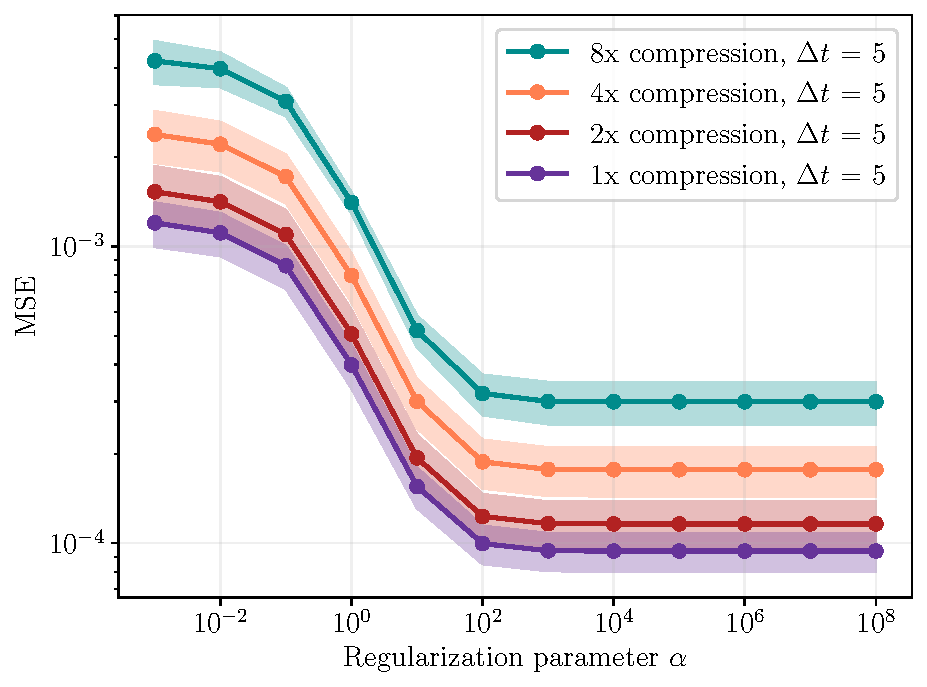
\includegraphics[width=\linewidth,height=0.52\textheight,keepaspectratio]{thesis/figures/chapter-5/fmri/subs_MSE_alpha.pdf}
    \par\footnotesize MSE от $\alpha$: оптимум $\alpha\approx1000$ сохраняется для всех сжатий.
\end{column}
\begin{column}{0.44\textwidth}
    \begin{itemize}
        \item $\boldsymbol{\psi}$: ResNet152 --- векторизация видео, $\mathbf{g}=\boldsymbol{\varphi}\circ\boldsymbol{\psi}$
        \item $\boldsymbol{\varphi}$: регрессия с $L_2$-регуляризацией, предсказание разности: $\hat{\mathbf{s}}_{\ell}=\mathbf{s}_{\ell-1}+\hat{\mathbf{W}}\mathbf{x}_{\ell}$
        \item сжатие $\boldsymbol{\chi}$ в $2^k$ раз без изменения архитектуры
    \end{itemize}
    \smallskip
    \begin{center}
    {\scriptsize\setlength{\tabcolsep}{4pt}
    \begin{tabular}{@{}cc@{}}
    \hline
    Сжатие & Время, с \\
    \hline
    $1$ & $36.3\pm6.1$ \\
    $2$ & $6.7\pm0.5$ \\
    $4$ & $1.6\pm0.1$ \\
    $8$ & $1.4\pm0.3$ \\
    \hline
    \end{tabular}}
    \end{center}
    \medskip
    сжатие в $8$ раз --- обучение в $\approx26$ раз быстрее при сохранении качества.
\end{column}
\end{columns}
\key{Снижение сложности данных сокращает время обучения при сохранении качества.}
\end{frame}
%----------------------------------------------------------------------------------------------------------
\begin{frame}{Качество данных: близость и устойчивость}
\justifying
\small
Метрики качества выборки $D$: близость распределений представлений и устойчивость к возмущениям.
\[
    \mathrm{KL}_{\mathrm{TTS}}(h_d,m_d)=\bigl|D_{\mathrm{KL}}(h_d\|m_d)-D_{\mathrm{KL}}(m_d\|h_d)\bigr|,
\]
\[
    \Delta_{\mathrm{shift}}=\log\frac{\frac{1}{n}\sum_i\cos_d\bigl(h^o_{h_i},h^p_{h_i}\bigr)}{\frac{1}{m}\sum_j\cos_d\bigl(h^o_{m_j},h^p_{m_j}\bigr)},\qquad
    \mathrm{KL}_{\mathrm{shuffle}}(H,M)=\sum_i H(i)\log\frac{H(i)}{M(i)}.
\]
\smallskip
\begin{itemize}
    \item чем ниже метрика --- тем ближе распределения и схожа устойчивость ($\mathrm{PHD}_{\mathrm{h}}$, $\mathrm{PHD}_{\mathrm{m}}$ --- средние попарные расстояния между представлениями в классах человеческого и сгенерированного текста).
    \item $F_1\approx1$ качества данных не гарантирует
\end{itemize}
\begin{center}
{\scriptsize\setlength{\tabcolsep}{4pt}
\begin{tabular}{@{}lccccc@{}}
\hline
Набор & $\mathrm{KL}_{\mathrm{TTS}}\downarrow$ & $\mathrm{PHD}_{\mathrm{h}}$ & $\mathrm{PHD}_{\mathrm{m}}$ & $\Delta_{\mathrm{shift}}\downarrow$ & $\mathrm{KL}_{\mathrm{shuffle}}\downarrow$ \\
\hline
MAGE & $\mathbf{0.011}$ & $9.8$ & $9.4$ & $0.094$ & $\mathbf{0.310}$ \\
SemEval24 Mono & $\mathbf{0.012}$ & $9.1$ & $9.4$ & $0.191$ & $2.576$ \\
RuATD & $0.007$ & $7.3$ & $7.5$ & $0.315$ & $14.028$ \\
\hline
\end{tabular}}
\end{center}
\smallskip
MAGE --- качественный набор ($\mathrm{KL}_{\mathrm{shuffle}}=0.31$, PHD близки), RuATD --- смещенный ($\mathrm{KL}_{\mathrm{shuffle}}=14.0$).
\key{Метрики качества данных эмпирически связаны с $\mu_f(f\mid D)$, но содержательная связь с ландшафтной мерой --- направление дальнейшего анализа.}
\end{frame}

%----------------------------------------------------------------------------------------------------------
\section{Выносится на защиту}
%----------------------------------------------------------------------------------------------------------
\begin{frame}{Результаты, выносимые на защиту}
\justifying
\footnotesize
\begin{enumerate}
    \justifying
    \setlength{\itemsep}{-2pt}
    \item Ландшафт полносвязной сети сходится при росте выборки со скоростью $O\bigl(L(hM)^{2L}/k\bigr)$.
    \item Скорость изменения эмпирического риска ограничена $A_1/(k+1)+2\varepsilon_gR$.
    \item Ковариация градиентов равна гаусс-ньютоновской компоненте Гессе, полный гессиан есть ее сумма с остатком.
    \item Мажоранта ландшафтной меры сложности полносвязной сети $\mu_f(f\mid D)\lesssim L(hM)^{2L}$: экспоненциальна по глубине, полиномиальна по ширине.
    \item Мажоранта ландшафтной меры сложности 1D-сверточной сети $\mu_f(f\mid D)\lesssim L(C^2M^2k_{\mathrm{ker}}d)^{L}$: полиномиальна степени $L$ по длине последовательности.
    \item Мажоранта ландшафтной меры сложности 2D-сверточной сети $\mu_f(f\mid D)\lesssim C^2k_{\mathrm{ker}}^2L(C^2k_{\mathrm{ker}}^2M^2mn)^{L}$: полиномиальна степени $L$ по площади изображения.
    \item Мажоранта ландшафтной меры сложности монотонна по глубине при $hM\ge1$ и не возрастает при макс- и усредняющем пулинге в предположении малости не-гаусс-ньютоновской компоненты гессиана.
    \item Достаточный размер выборки~$m^*$ ограничен с двух сторон через меру разброса Гессе и ландшафтную меру сложности.
    \item Достаточный размер выборки $m^*=\Theta\bigl((M_\ell+\mu_f(f\mid D)R^2)/\varepsilon\bigr)$: пропорционален мере сложности, обратно пропорционален точности.
    \item Оценка при низкоранговой адаптации состоятельна.
    \item При многозадачном обучении верхние оценки радемахеровской сложности на задачу сравнимы и при условиях (С2)–(С4) влекут уменьшение достаточного размера выборки.
\end{enumerate}
\end{frame}
%----------------------------------------------------------------------------------------------------------
\begin{frame}{Положения, выносимые на защиту}
\justifying
\normalsize
\begin{enumerate}
    \justifying
    \setlength{\itemsep}{-1pt}
    \item Мера сложности модели и монотонная субаддитивная мера сложности выборки вместе с критерием их согласованности задают формальный аппарат соответствия параметрической модели характеристикам обучающей выборки, а условная сложность выборки выражается через достаточный размер выборки, что делает критерий порядковым и применимым для сопоставления моделей и выборок.
    \item Ландшафтная мера сложности модели количественно связывает архитектуру модели с изменением эмпирического риска при изменении выборки.
    \item Верхние оценки ландшафтной меры сложности модели следуют из единого факторизованного представления матрицы Гессе и растут экспоненциально с глубиной сети и полиномиально с шириной и числом каналов. Для слоя самовнимания получена оценка по компонентам, полиномиальная по норме входов и нормам весов.
    \item Достаточный размер выборки определяется ландшафтной мерой сложности модели и требуемой точностью аппроксимации, причем верхняя оценка размера выборки пропорциональна этой мере и обратно пропорциональна точности.
    \item Снижение размерности пространства обучаемых параметров уменьшает эффективную сложность модели при сохранении качества прогноза и классификации и незначительном изменении метрик качества аппроксимации.
\end{enumerate}
\end{frame}
%----------------------------------------------------------------------------------------------------------
\begin{frame}{Соответствие паспорту специальности 1.2.1}
\justifying
\begin{center}
\begin{tabular}{|p{0.7\textwidth}|c|}
\hline
\textbf{Пункт паспорта} & \textbf{Положение} \\
\hline
2. Исследования в области оценки качества и эффективности алгоритмических и программных решений для систем искусственного интеллекта и машинного обучения. Методики сравнения и выбора алгоритмических и программных решений при многих критериях. & 1, 4, 5 \\
\hline
4. Разработка методов, алгоритмов и создание систем искусственного интеллекта и машинного обучения для обработки и анализа текстов на естественном языке, для изображений, речи, биомедицины и других специальных видов данных. & 5 \\
\hline
16. Исследования в области специальных методов оптимизации, проблем сложности и элиминации перебора, снижения размерности. & 1, 2, 4, 5 \\
\hline
17. Исследования в области многослойных алгоритмических конструкций, в том числе многослойных нейросетей. & 2, 3 \\
\hline
\end{tabular}
\end{center}
\end{frame}
%----------------------------------------------------------------------------------------------------------
\begin{frame}{Публикации по теме диссертации}
\justifying
\normalsize
По теме диссертации опубликовано 66 научных работ, в том числе: 25 статей в журналах перечня ВАК, 30 --- в изданиях Scopus и Web of Science, 39 --- в трудах российских и международных конференций.
\begin{enumerate}
\tiny
\setlength{\leftmargin}{1.2em}
\setlength{\itemsep}{-0.6pt}
    \item \textbf{Грабовой}~А.\,В. От VC-размерности к законам масштабирования: эволюция теоретических подходов к оценке сложности и обобщающей способности // Интеллектуальные системы. Теория и приложения. 2026.
    \item \textbf{Grabovoy}~A.\,V. Landscape Measure of Deep Learning Models // Pattern Recognition and Image Analysis: Advances in Mathematical Theory and Applications. 2026.
    \item Kiselev~N.\,S., Meshkov~V.\,S., \textbf{Grabovoy}~A.\,V. Устойчивая сходимость поверхности функции потерь через усреднение по распределению // Труды Института системного программирования РАН. 2026.
    \item Kiselev~N.\,S., \textbf{Grabovoy}~A.\,V. Unraveling the Hessian: A Key to Smooth Convergence in Loss Function Landscapes // Doklady Mathematics. 2024.
    \item Kiselev~N.\,S., \textbf{Grabovoy}~A.\,V. Sample Size Determination: Likelihood Bootstrapping // Computational Mathematics and Mathematical Physics. 2025.
    \item Kiselev~N., \textbf{Grabovoy}~A. Sample size determination: posterior distributions proximity // Computational Management Science. 2025.
    \item \textbf{Grabovoy}~A.\,V., Gadaev~T.\,T., Motrenko~A.\,P., Strijov~V.\,V. Numerical Methods of Sufficient Sample Size Estimation for Generalised Linear Models // Lobachevskii Journal of Mathematics. 2022.
    \item \textbf{Grabovoy}~A.\,V., Strijov~V.\,V. Probabilistic Interpretation of the Distillation Problem // Automation and Remote Control. 2022.
    \item \textbf{Grabovoy}~A.\,V., Strijov~V.\,V. Bayesian Distillation of Deep Learning Models // Automation and Remote Control. 2021.
    \item \textbf{Грабовой}~А.\,В., Бахтеев~О.\,Ю., Стрижов~В.\,В. Введение отношения порядка на множестве параметров аппроксимирующих моделей // Информатика и ее применения. 2020.
    \item \textbf{Грабовой}~А.\,В., Бахтеев~О.\,Ю., Стрижов~В.\,В. Определение релевантности параметров нейросети // Информатика и ее применения. 2019.
    \item \textbf{Grabovoy}~A.\,V., Strijov~V.\,V. Prior Distribution Selection for a Mixture of Experts // Computational Mathematics and Mathematical Physics. 2021.
    \item Meshkov~V., Kiselev~N., \textbf{Grabovoy}~A. ConvNets Landscape Convergence: Hessian-Based Analysis of Matricized Networks // 2024 Ivannikov Ispras Open Conference (ISPRAS). 2024.
    \item Petrushina~K., Bakhteev~O., \textbf{Grabovoy}~A., Strijov~V. Anti-Distillation: Knowledge Transfer from a Simple Model to the Complex One // 2022 Ivannikov Ispras Open Conference (ISPRAS). 2022.
    \item Dorin~D., Kiselev~N., \textbf{Grabovoy}~A., Strijov~V. Forecasting fMRI images from video sequences: linear model analysis // Health Information Science and Systems. 2024.
\end{enumerate}
\end{frame}
%----------------------------------------------------------------------------------------------------------
\end{document}